The question we have is wheter the SM Higgs boson exists or not.  
This chapter discusses the interpretation of data to answer this question.

For the cut-based method, the table of yields and the distributions 
of \mT\ and \mll\ after Higgs selection are shown. 
For the shape-based method, the 2-dimensional and the $\frac{S}{S+B}$-weighted 1-dimensional
data - backgrounds plots are shown to see by eye to check the 
compatibility of data with the \mHi=125~\GeV\ hypothesis. 
Then, the exclusion limit and the significance are shown combining 
shape-based and cut-based results in \DF\ and \SF\ categories, respectivley, 
using 7 and 8~\TeV\ data. Finally, the measurement on the 
production rate in terms of the signal strength is discussed. 


\section{Cut-based Method results}  
%%%%% cut-based result %%%%%

Figure~\ref{fig:cutbased125_0jet} and \ref{fig:cutbased125_1jet} show the
\mT\ and \mll\ distributions with the \mHi=125~\GeV\ selection 
in the 0-jet and 1-jet categories, respectively. 
All lepton final states, \DF, \SF and inclusive category from the top, are shown. 
Table~\ref{tab:cut7tev} and \ref{tab:cut8tev} show the yields of each process 
in 7 and 8~\TeV, repectively.
The data shows a good agreement with the assumption of \mHi=125~\GeV\ Higgs boson. 

\begin{figure}[htp] 
\centering 
\begin{tabular}{c} 
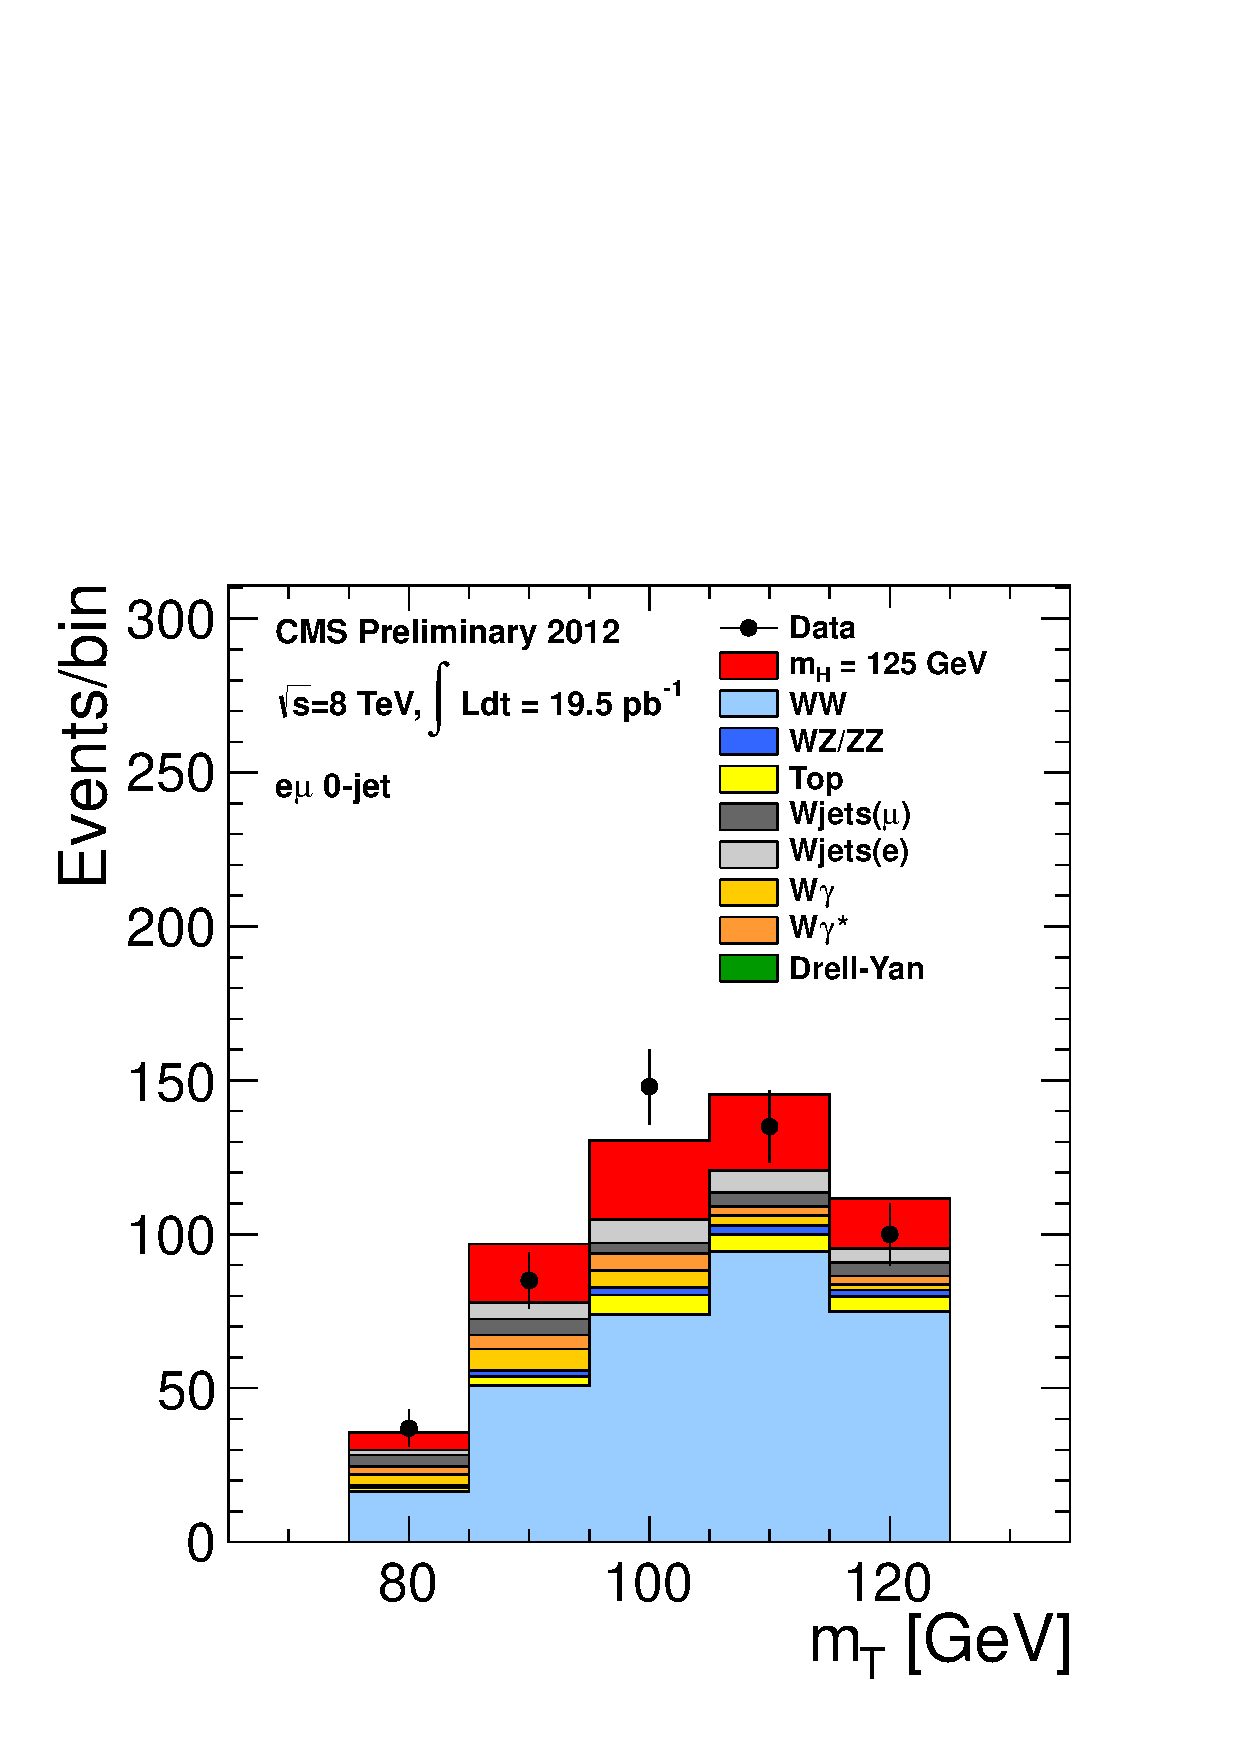
\includegraphics[width=0.45\textwidth]{figures/hww_analysis17_125_ALL_of_0j_mt.pdf}
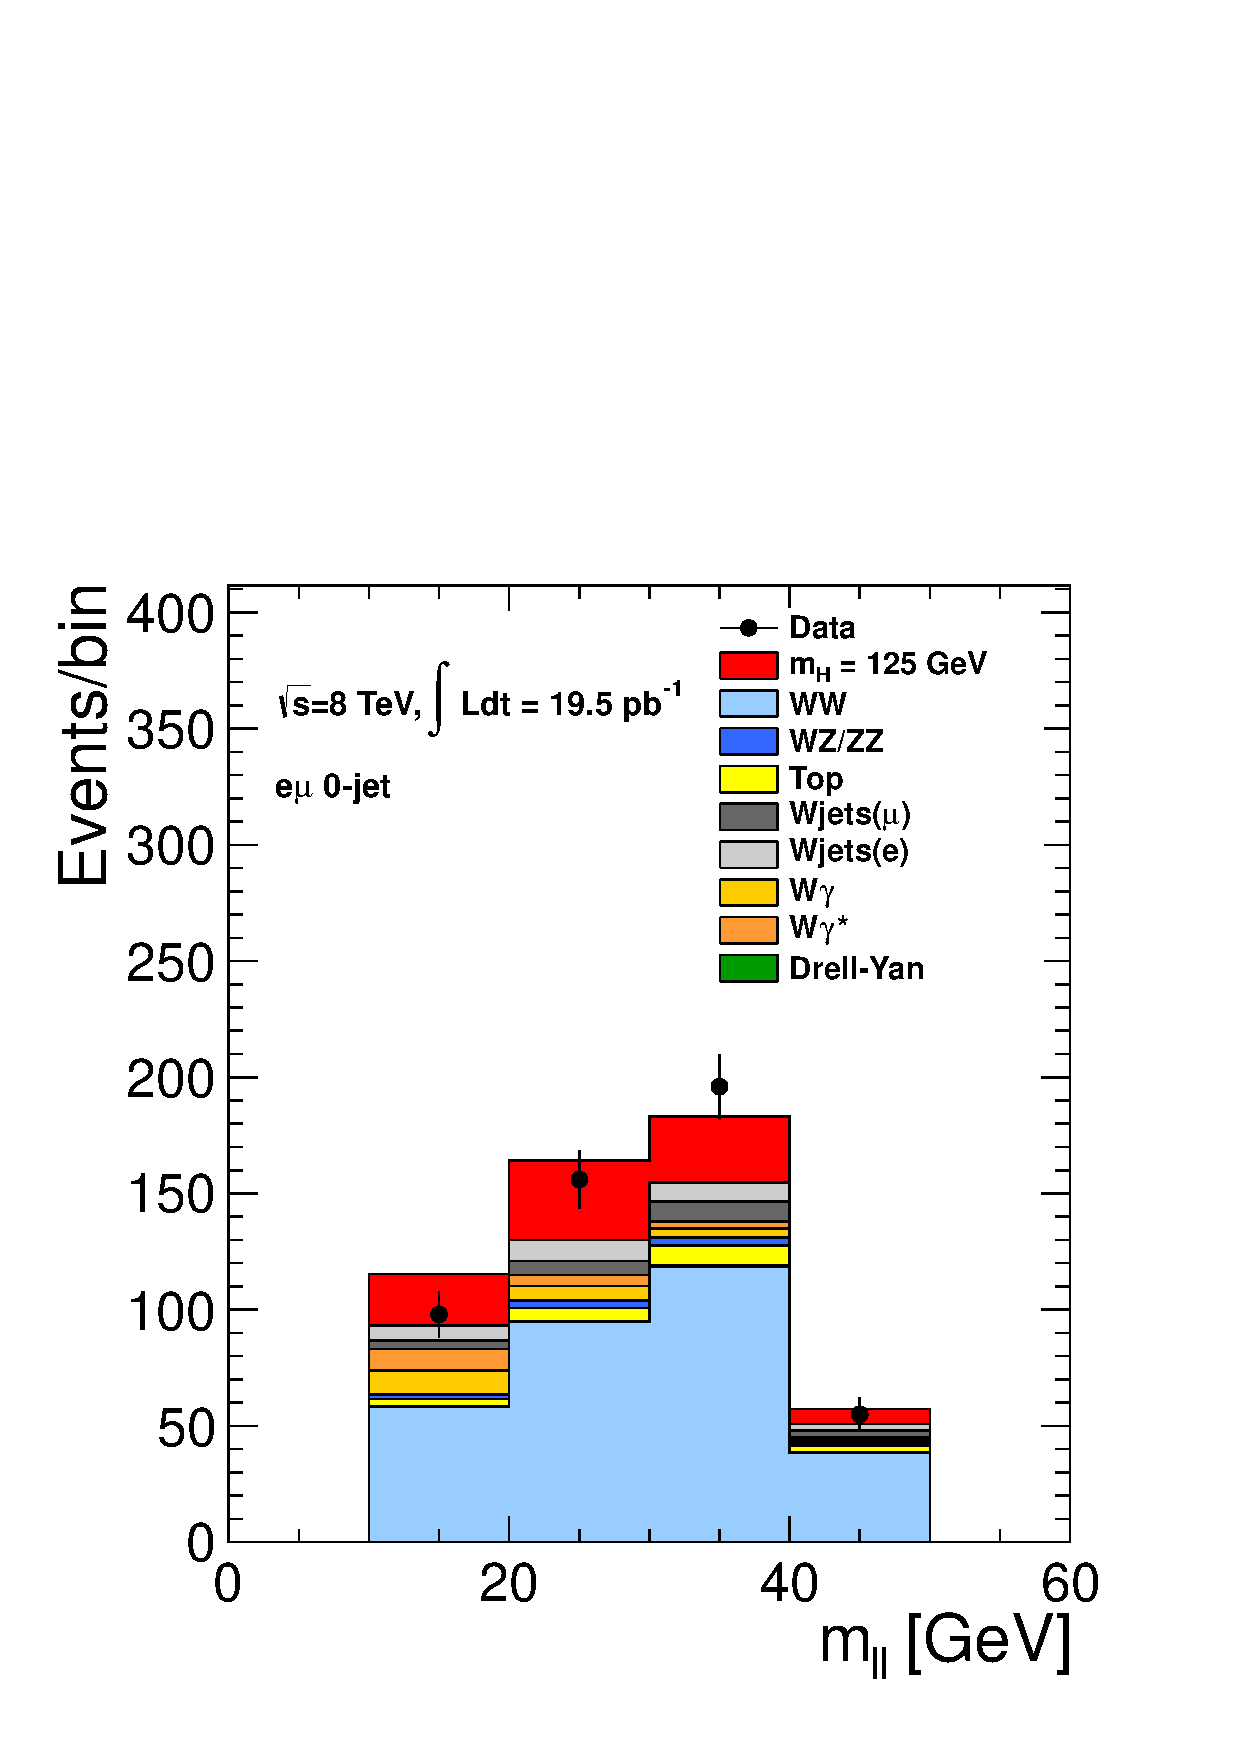
\includegraphics[width=0.45\textwidth]{figures/hww_analysis17_125_ALL_of_0j_mll.pdf} 
\\
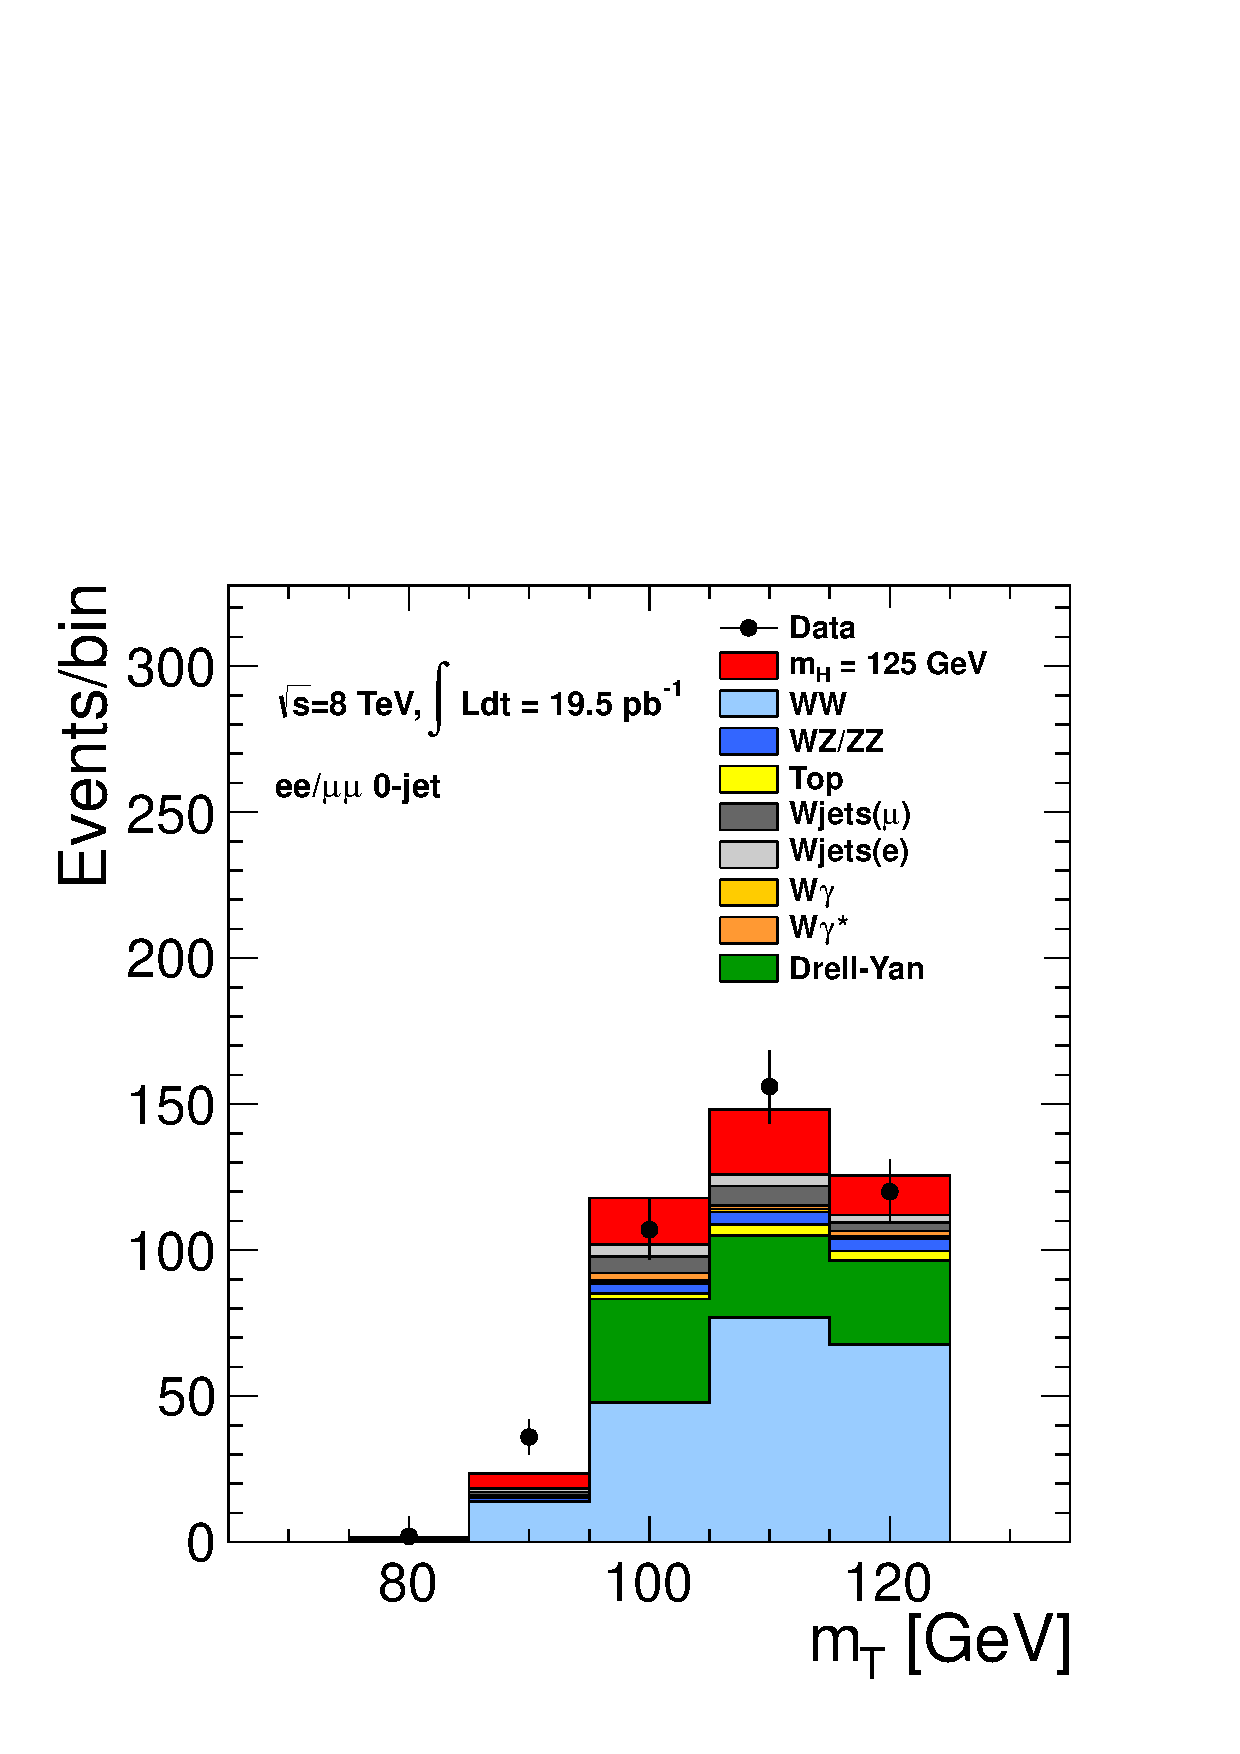
\includegraphics[width=0.45\textwidth]{figures/hww_analysis17_125_ALL_sf_0j_mt.pdf}
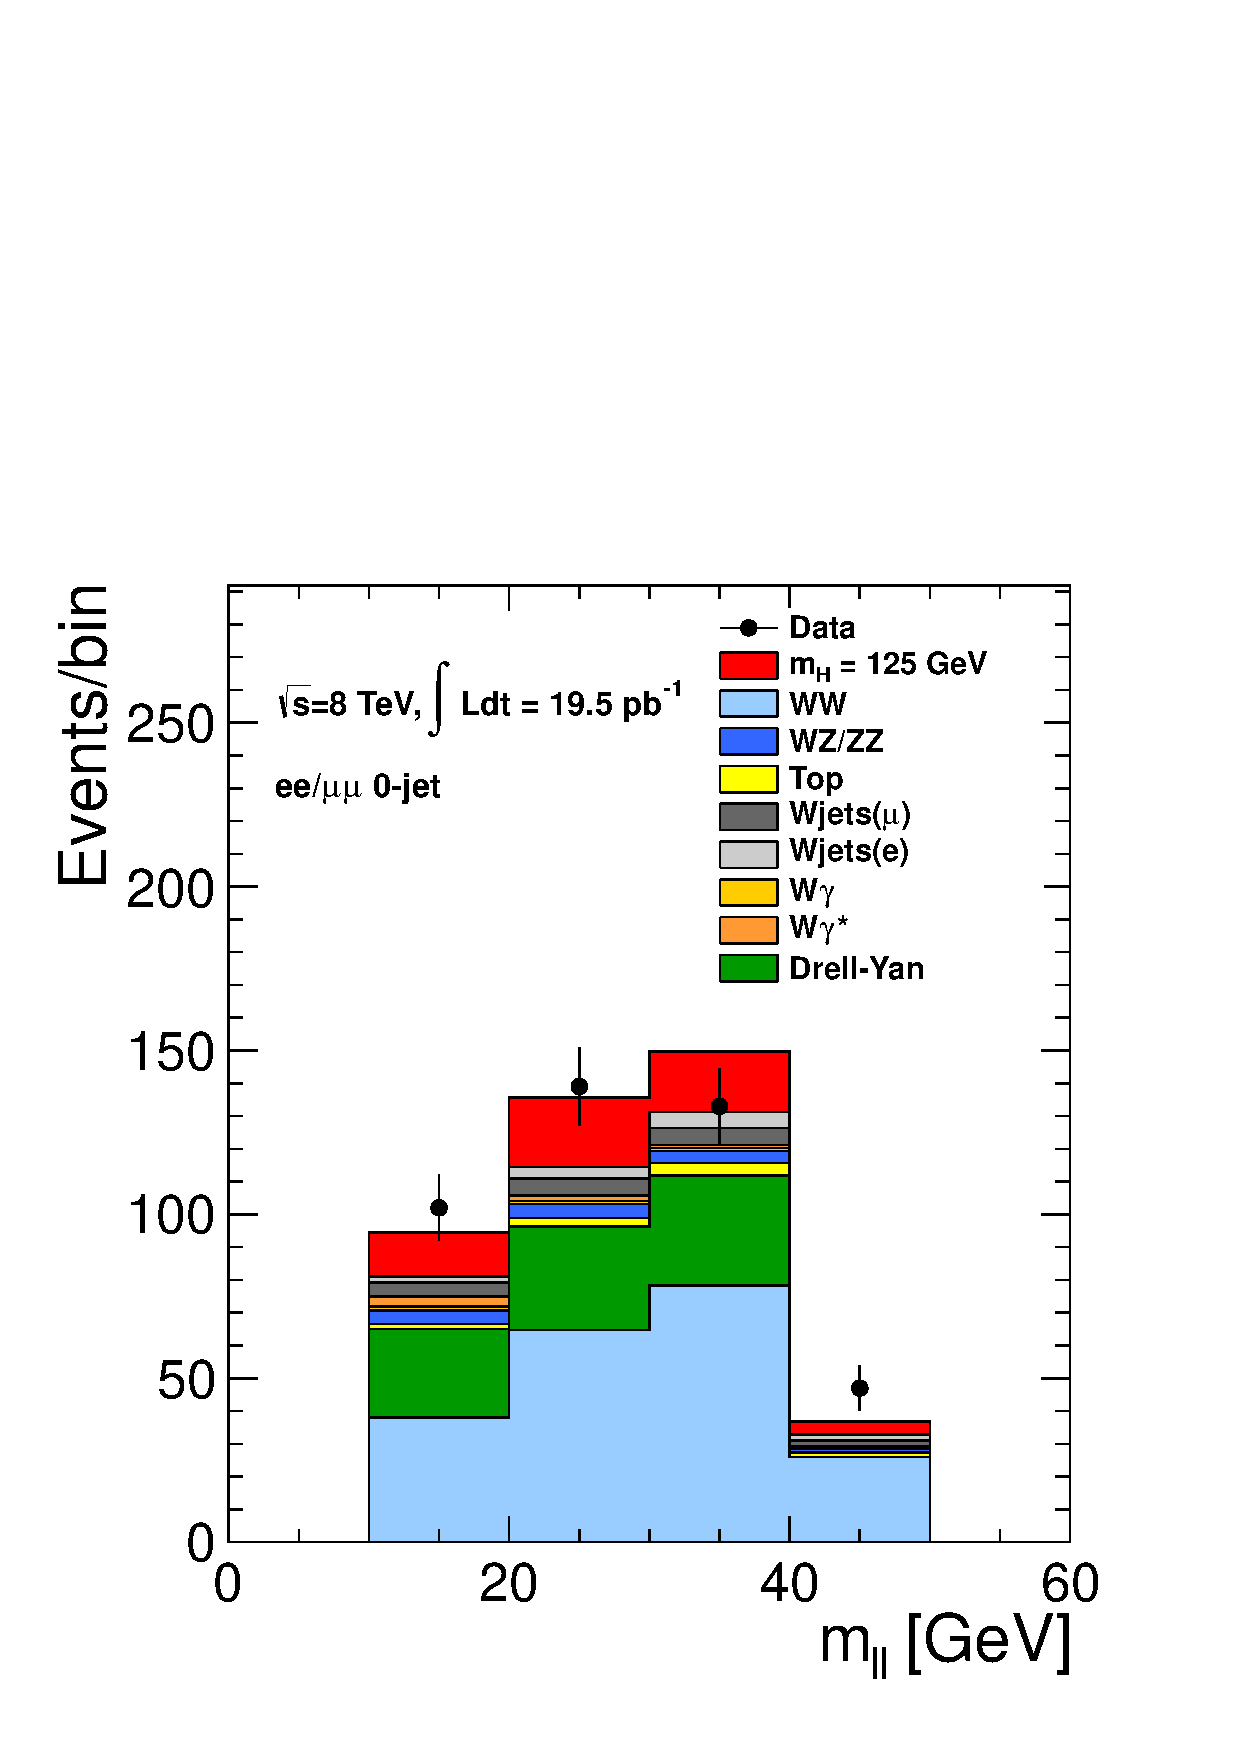
\includegraphics[width=0.45\textwidth]{figures/hww_analysis17_125_ALL_sf_0j_mll.pdf}
\\
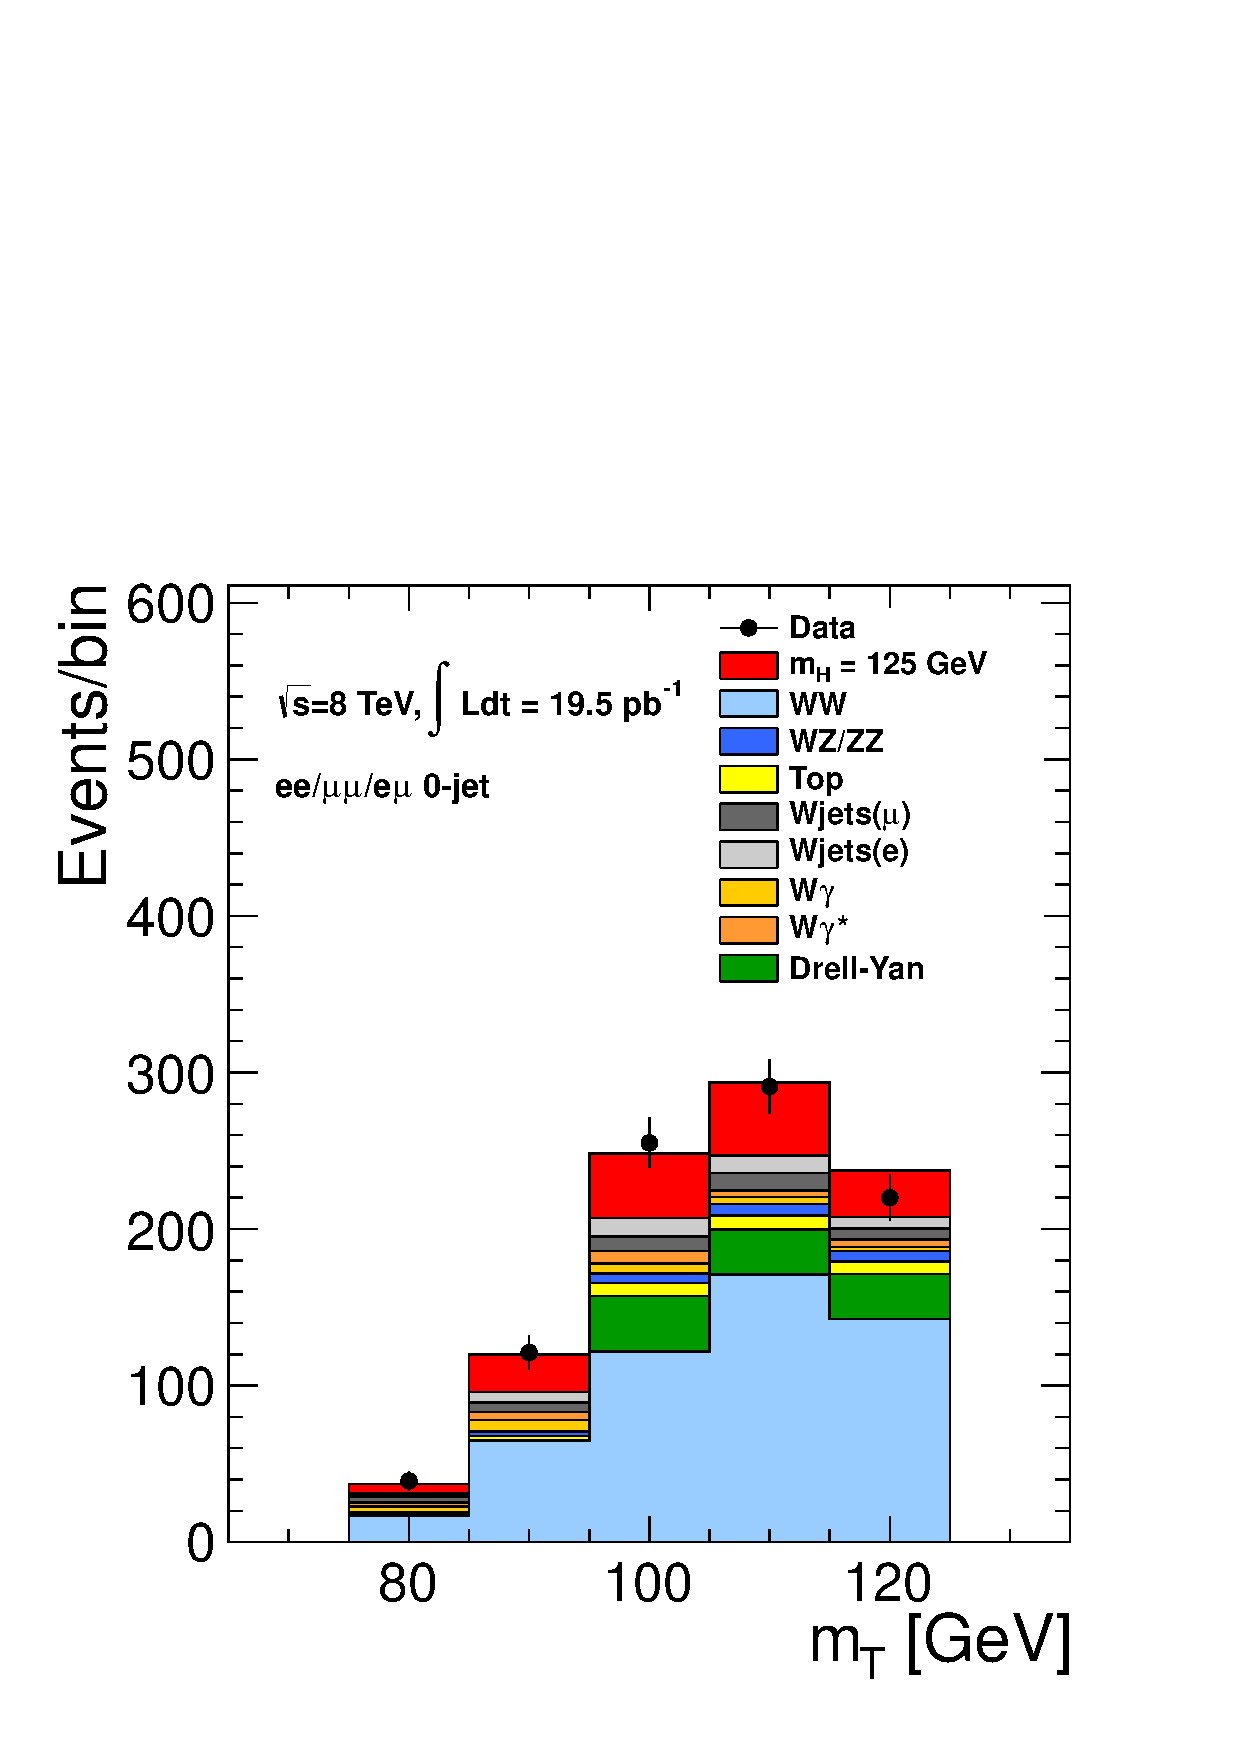
\includegraphics[width=0.45\textwidth]{figures/hww_analysis17_125_ALL_incl_0j_mt.pdf}
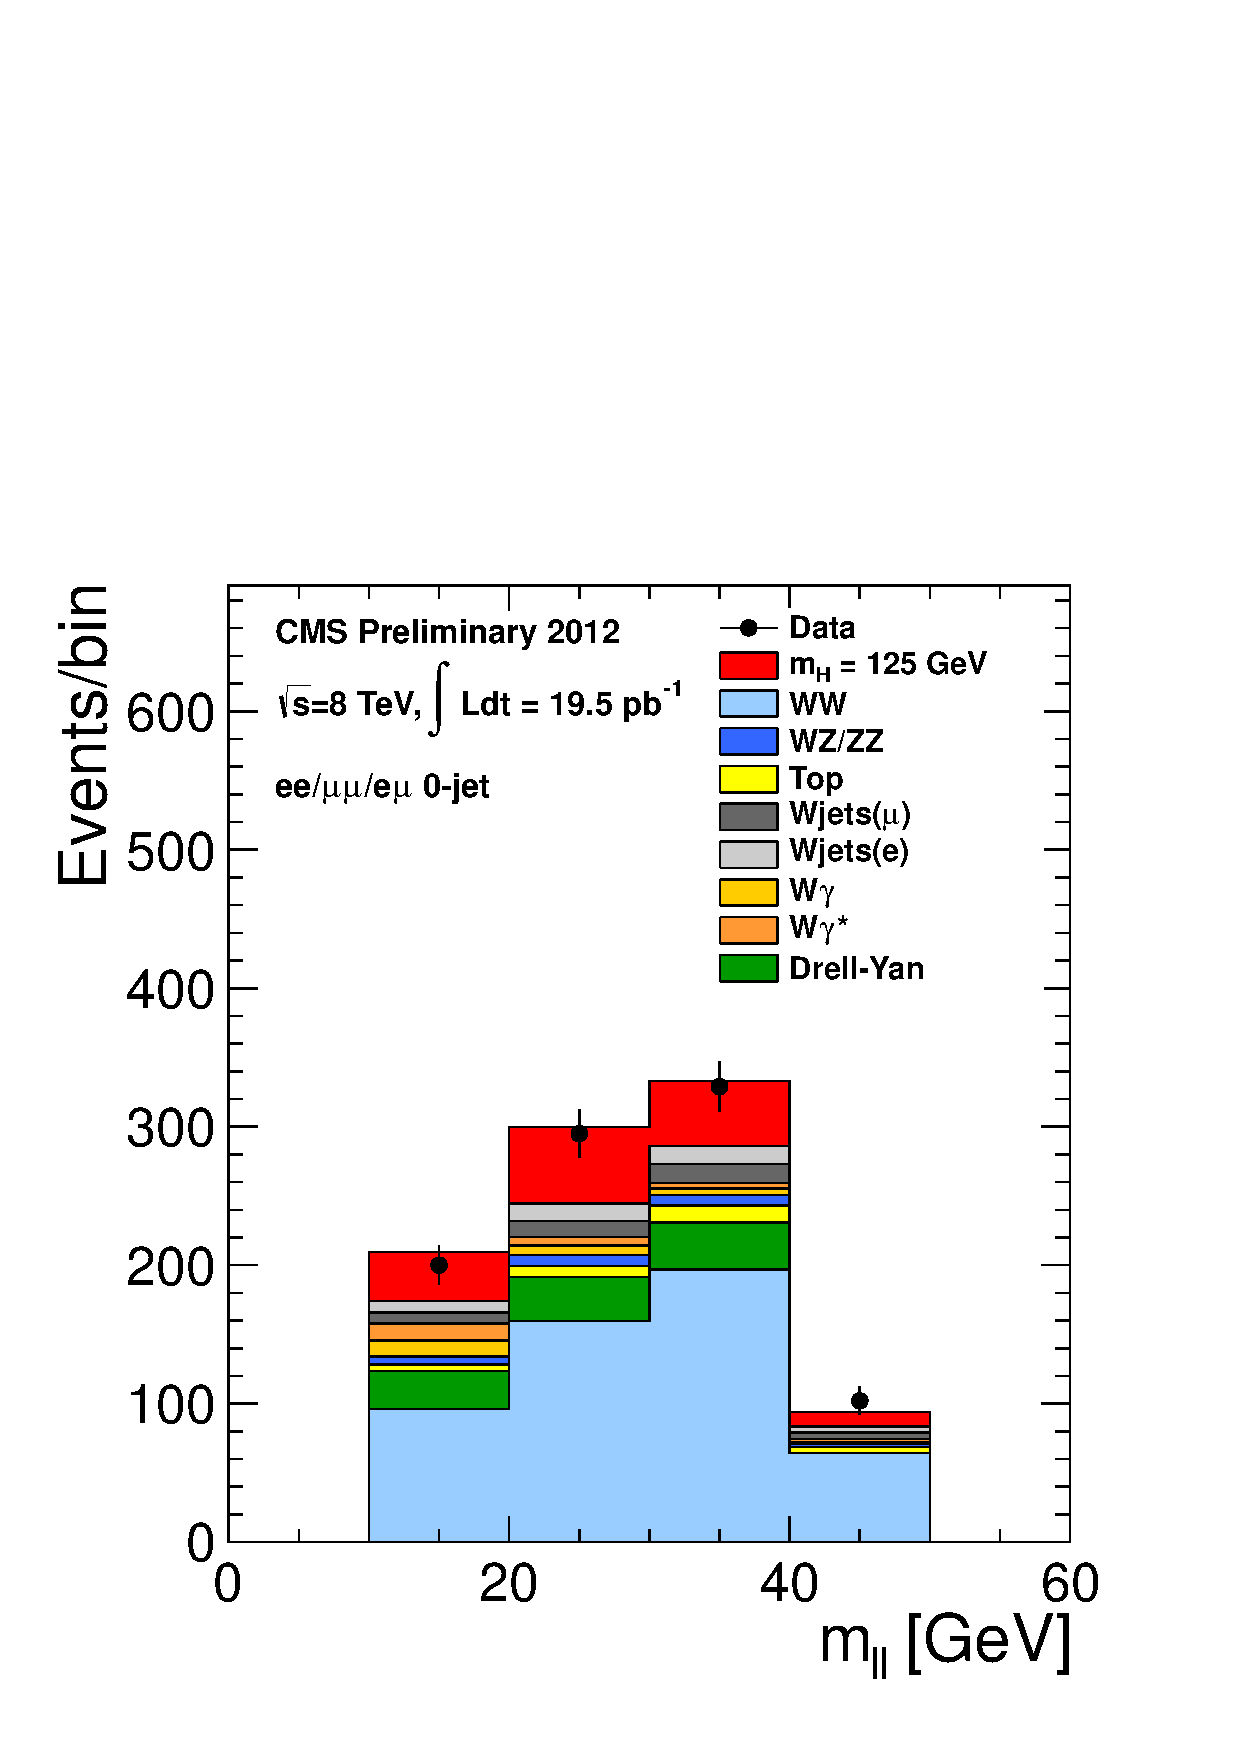
\includegraphics[width=0.45\textwidth]{figures/hww_analysis17_125_ALL_incl_0j_mll.pdf}
\end{tabular} 
\caption{ \mT(left) and \mll(right) distributionss for \mHi=125~\GeV\ analysis 
in 0-jet category. 
Top is for \DF, middle is for \SF, and the bottom is for the inclusive channel.  
The data shows good agreement bewteen prediction assmuing \mHi=125~\GeV\ Higgs boson.} 
\label{fig:cutbased125_0jet} 
\end{figure} 
%
\begin{figure}[htp] 
\centering 
\begin{tabular}{c} 
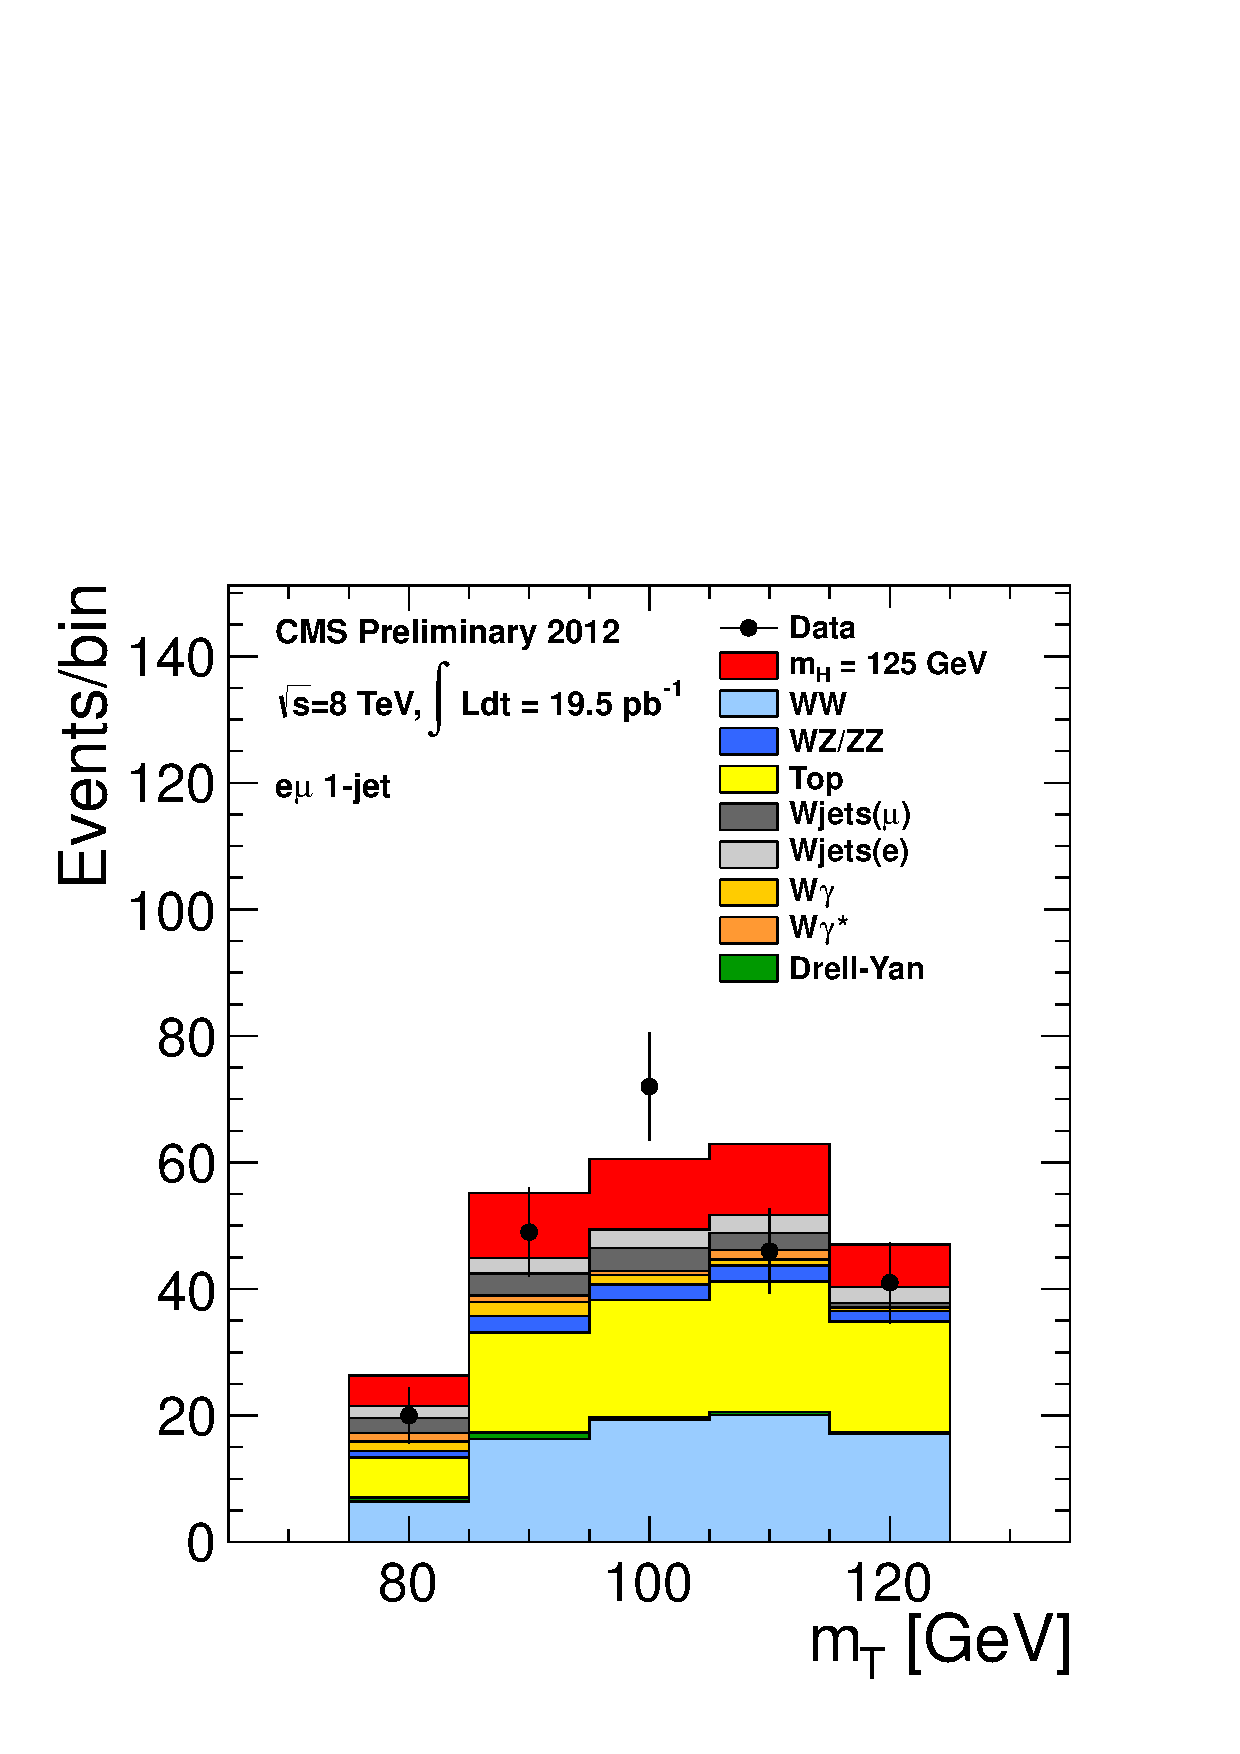
\includegraphics[width=0.45\textwidth]{figures/hww_analysis17_125_ALL_of_1j_mt.pdf}
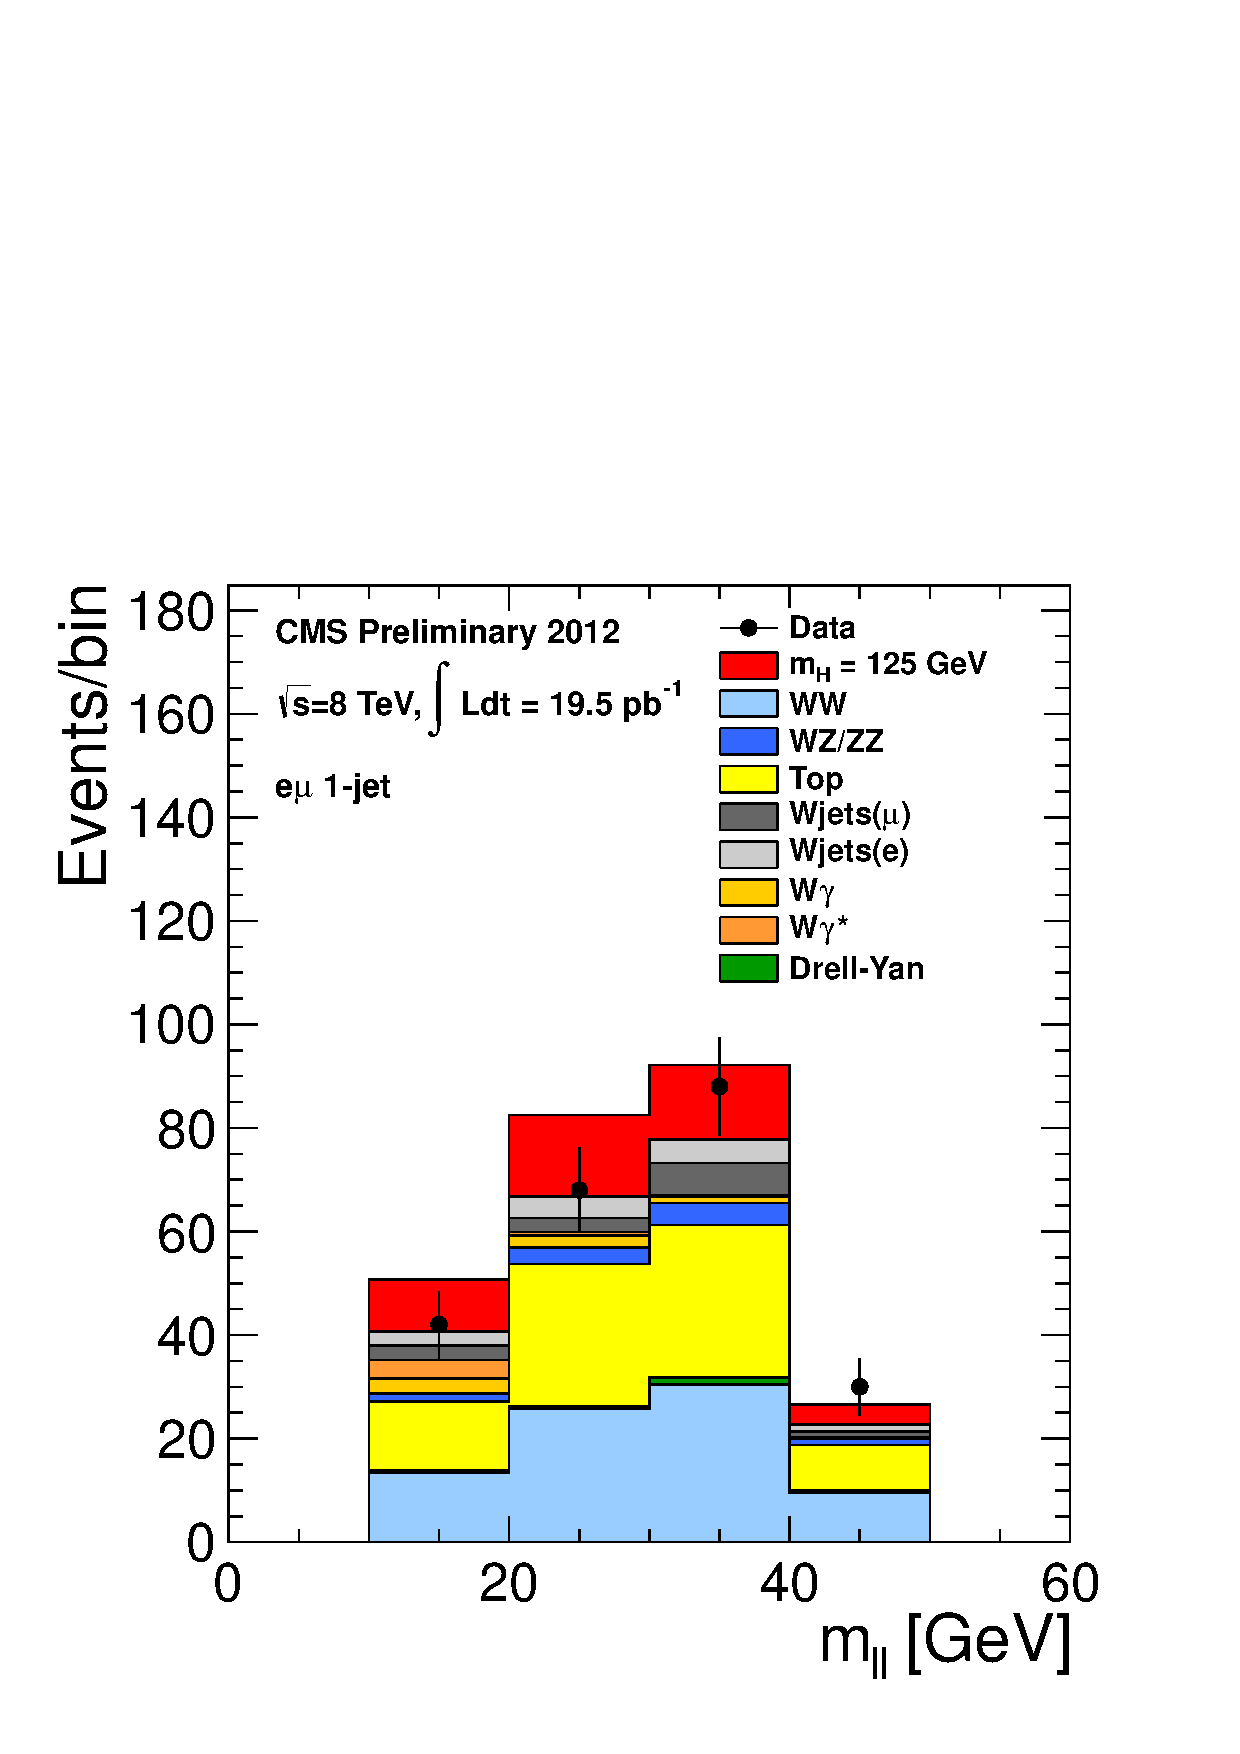
\includegraphics[width=0.45\textwidth]{figures/hww_analysis17_125_ALL_of_1j_mll.pdf} 
\\
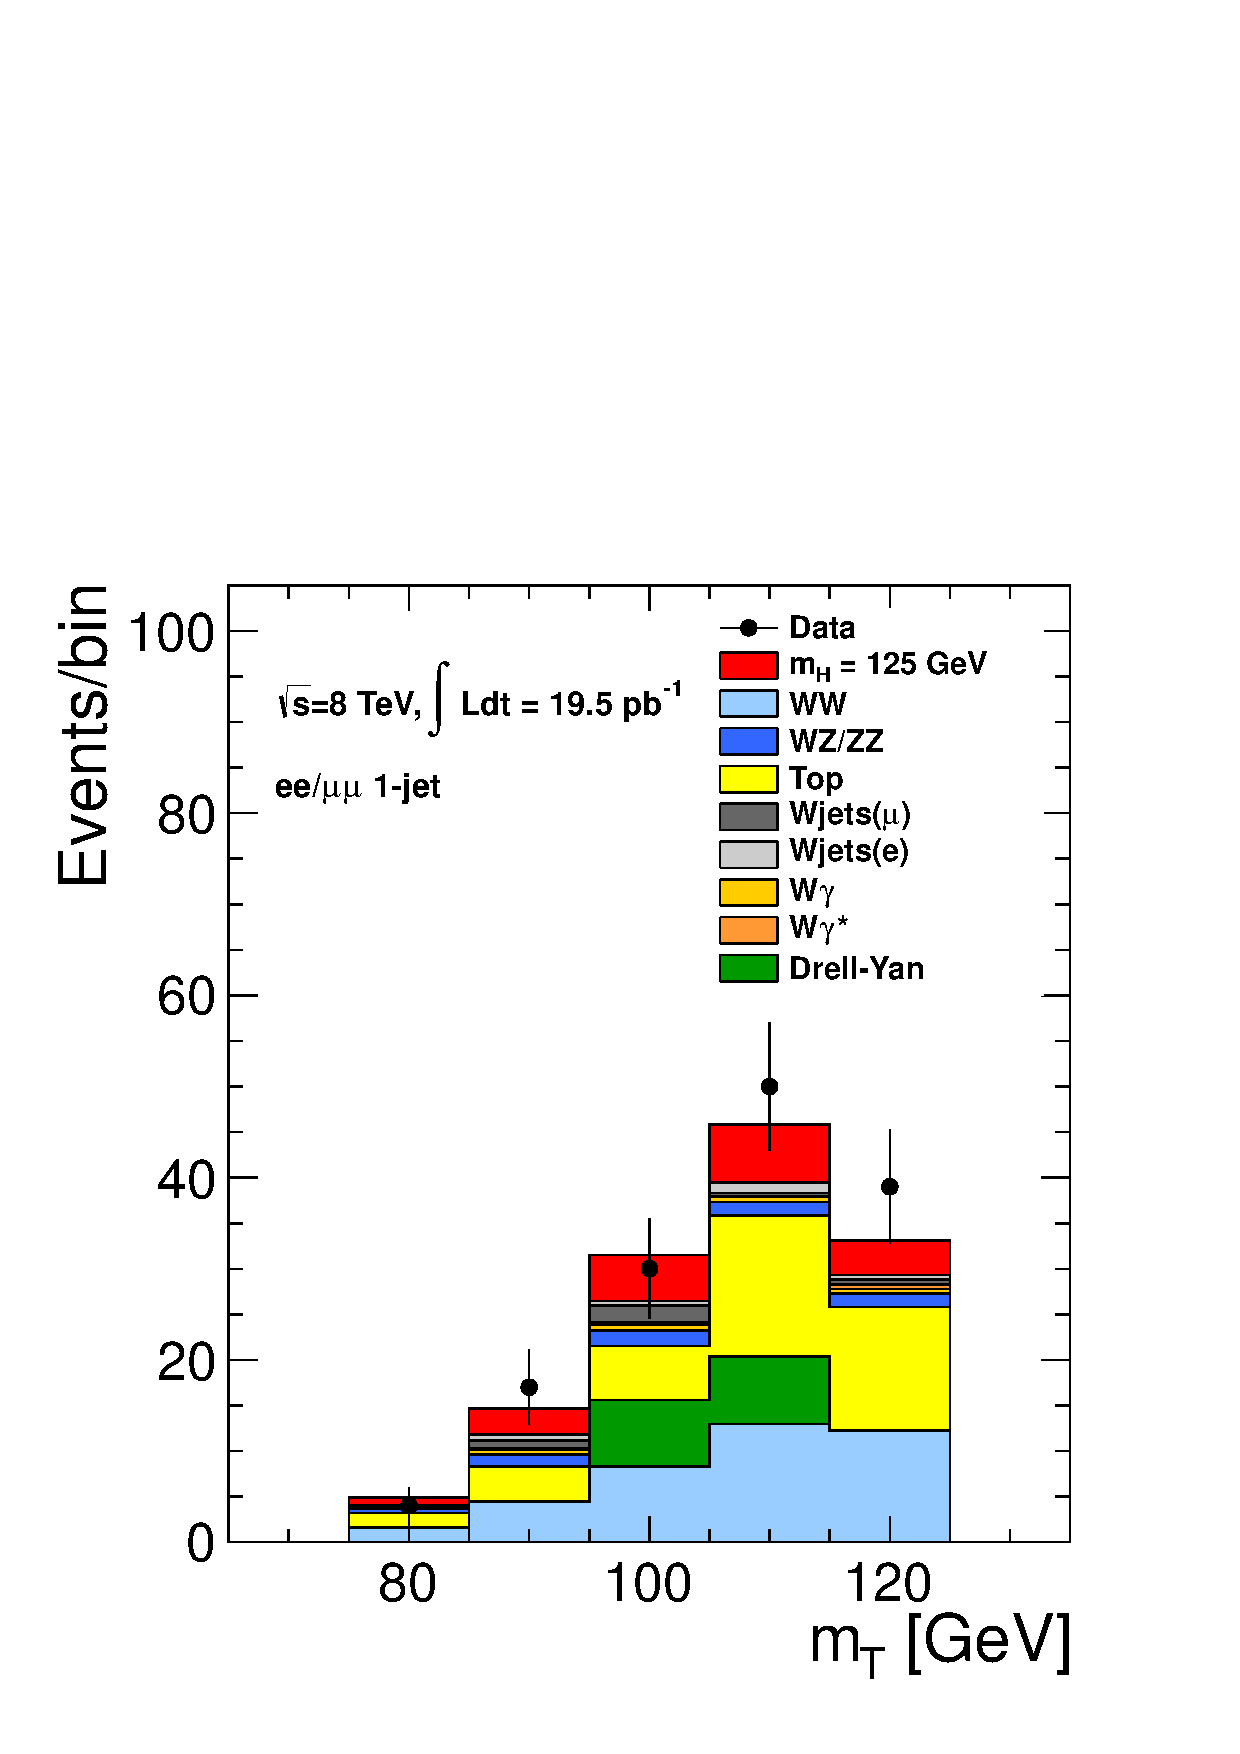
\includegraphics[width=0.45\textwidth]{figures/hww_analysis17_125_ALL_sf_1j_mt.pdf}
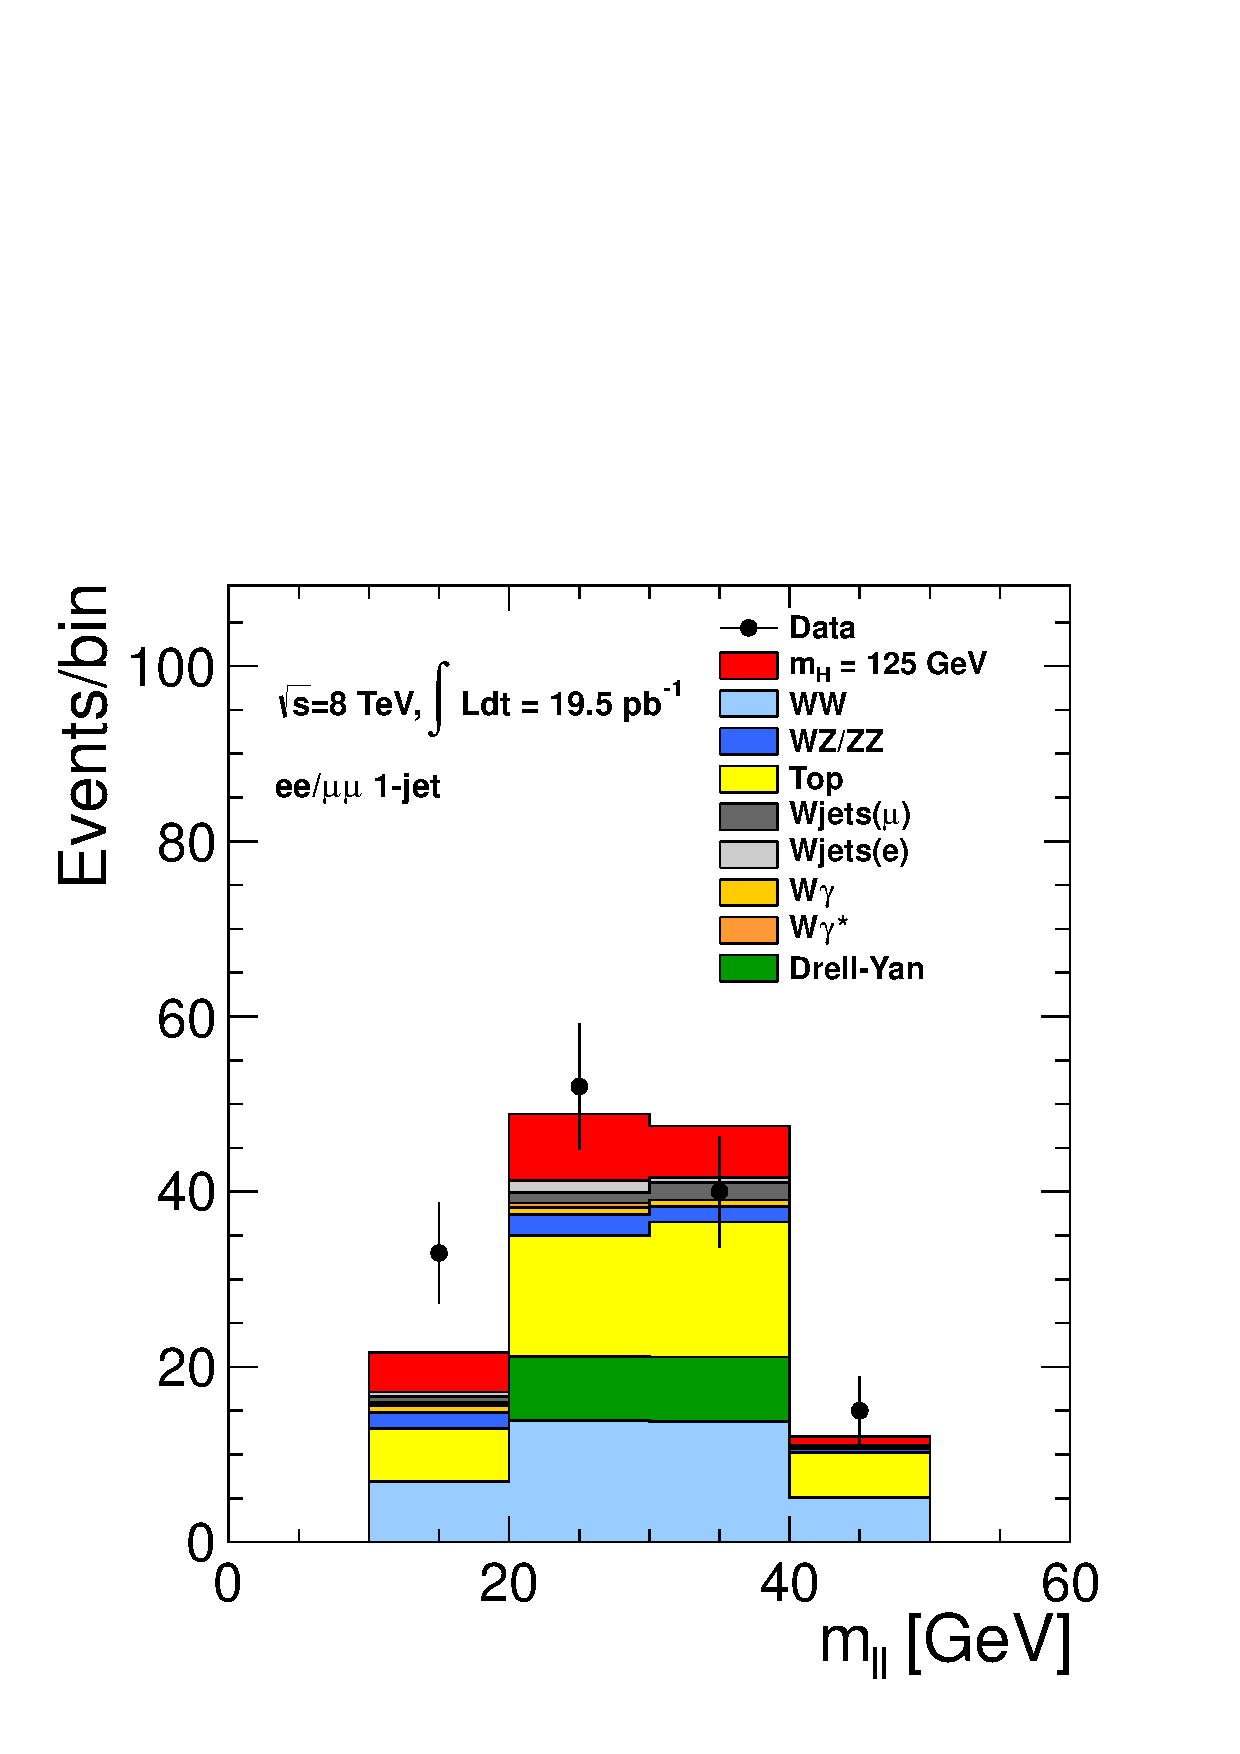
\includegraphics[width=0.45\textwidth]{figures/hww_analysis17_125_ALL_sf_1j_mll.pdf}
\\
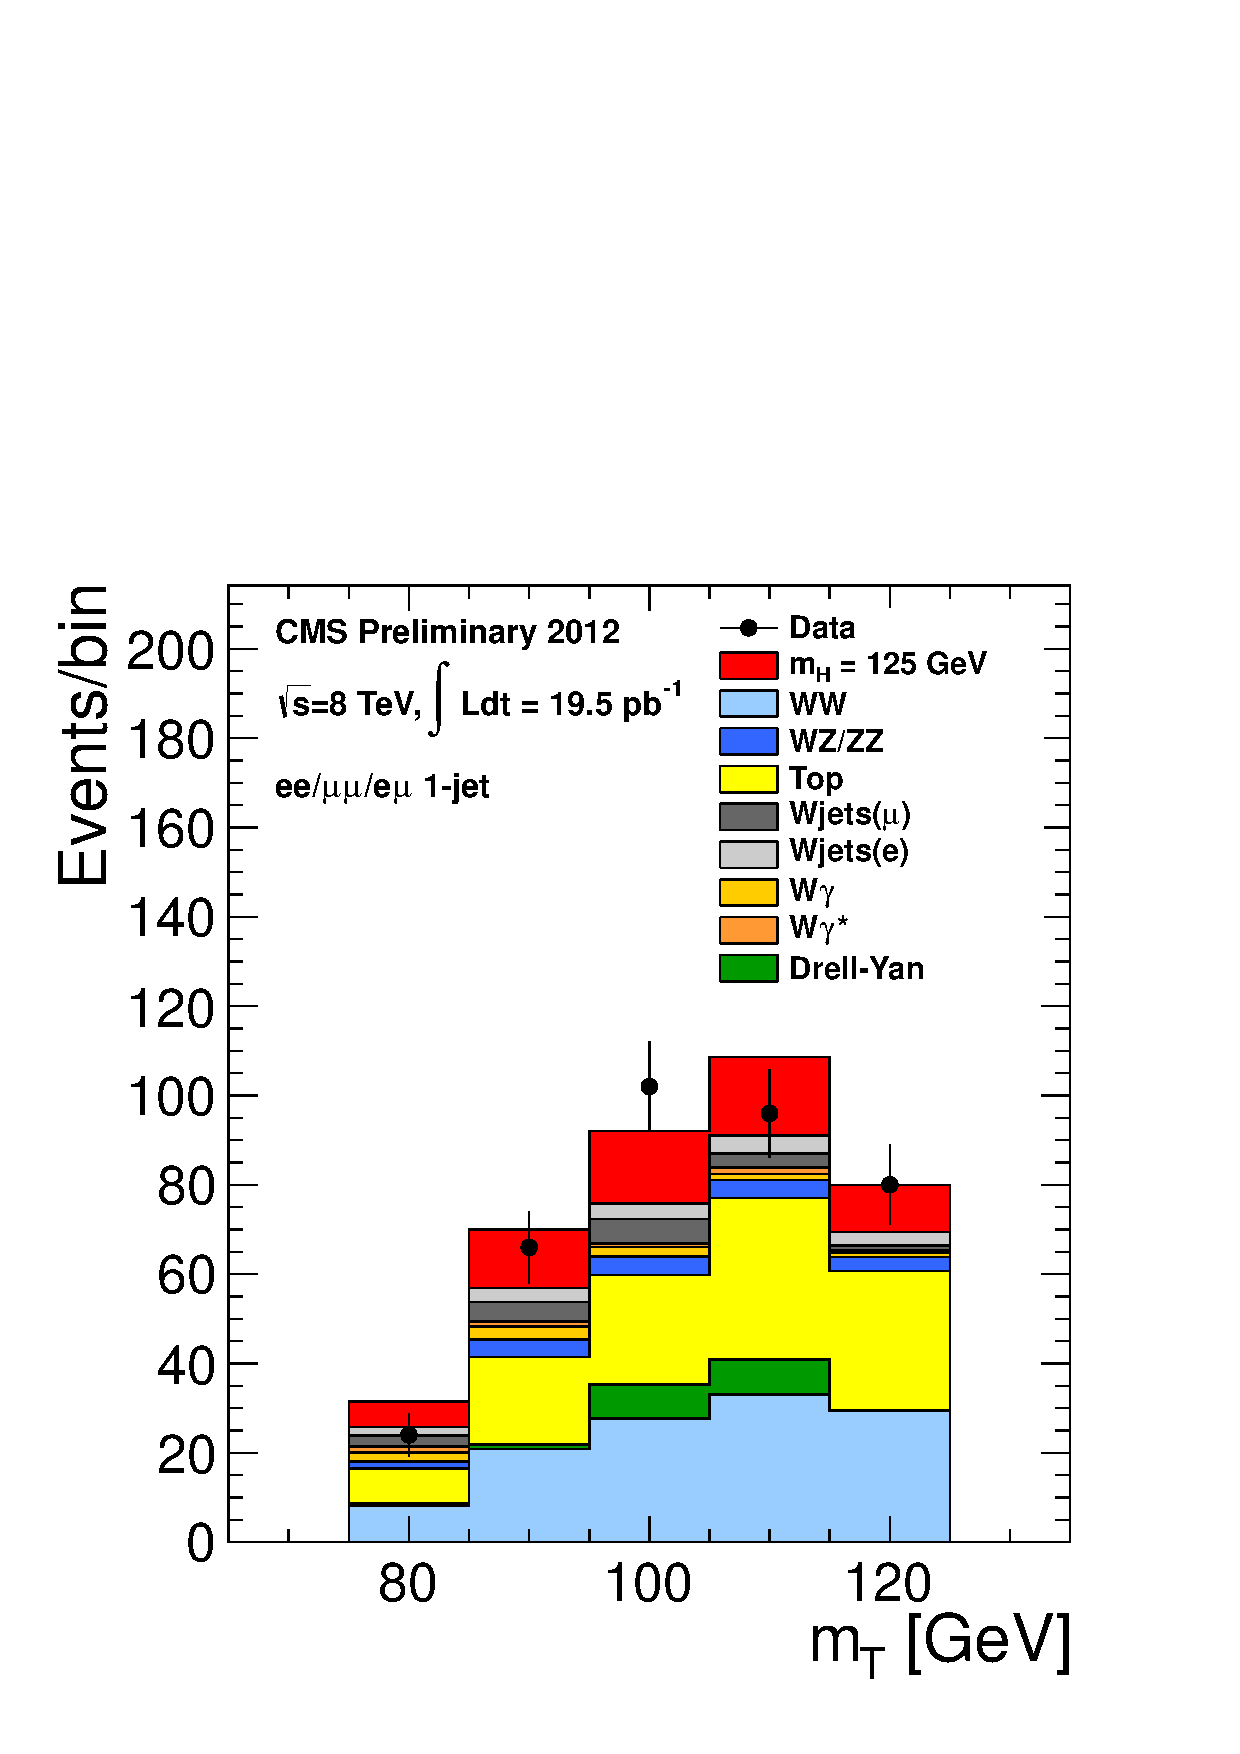
\includegraphics[width=0.45\textwidth]{figures/hww_analysis17_125_ALL_incl_1j_mt.pdf}
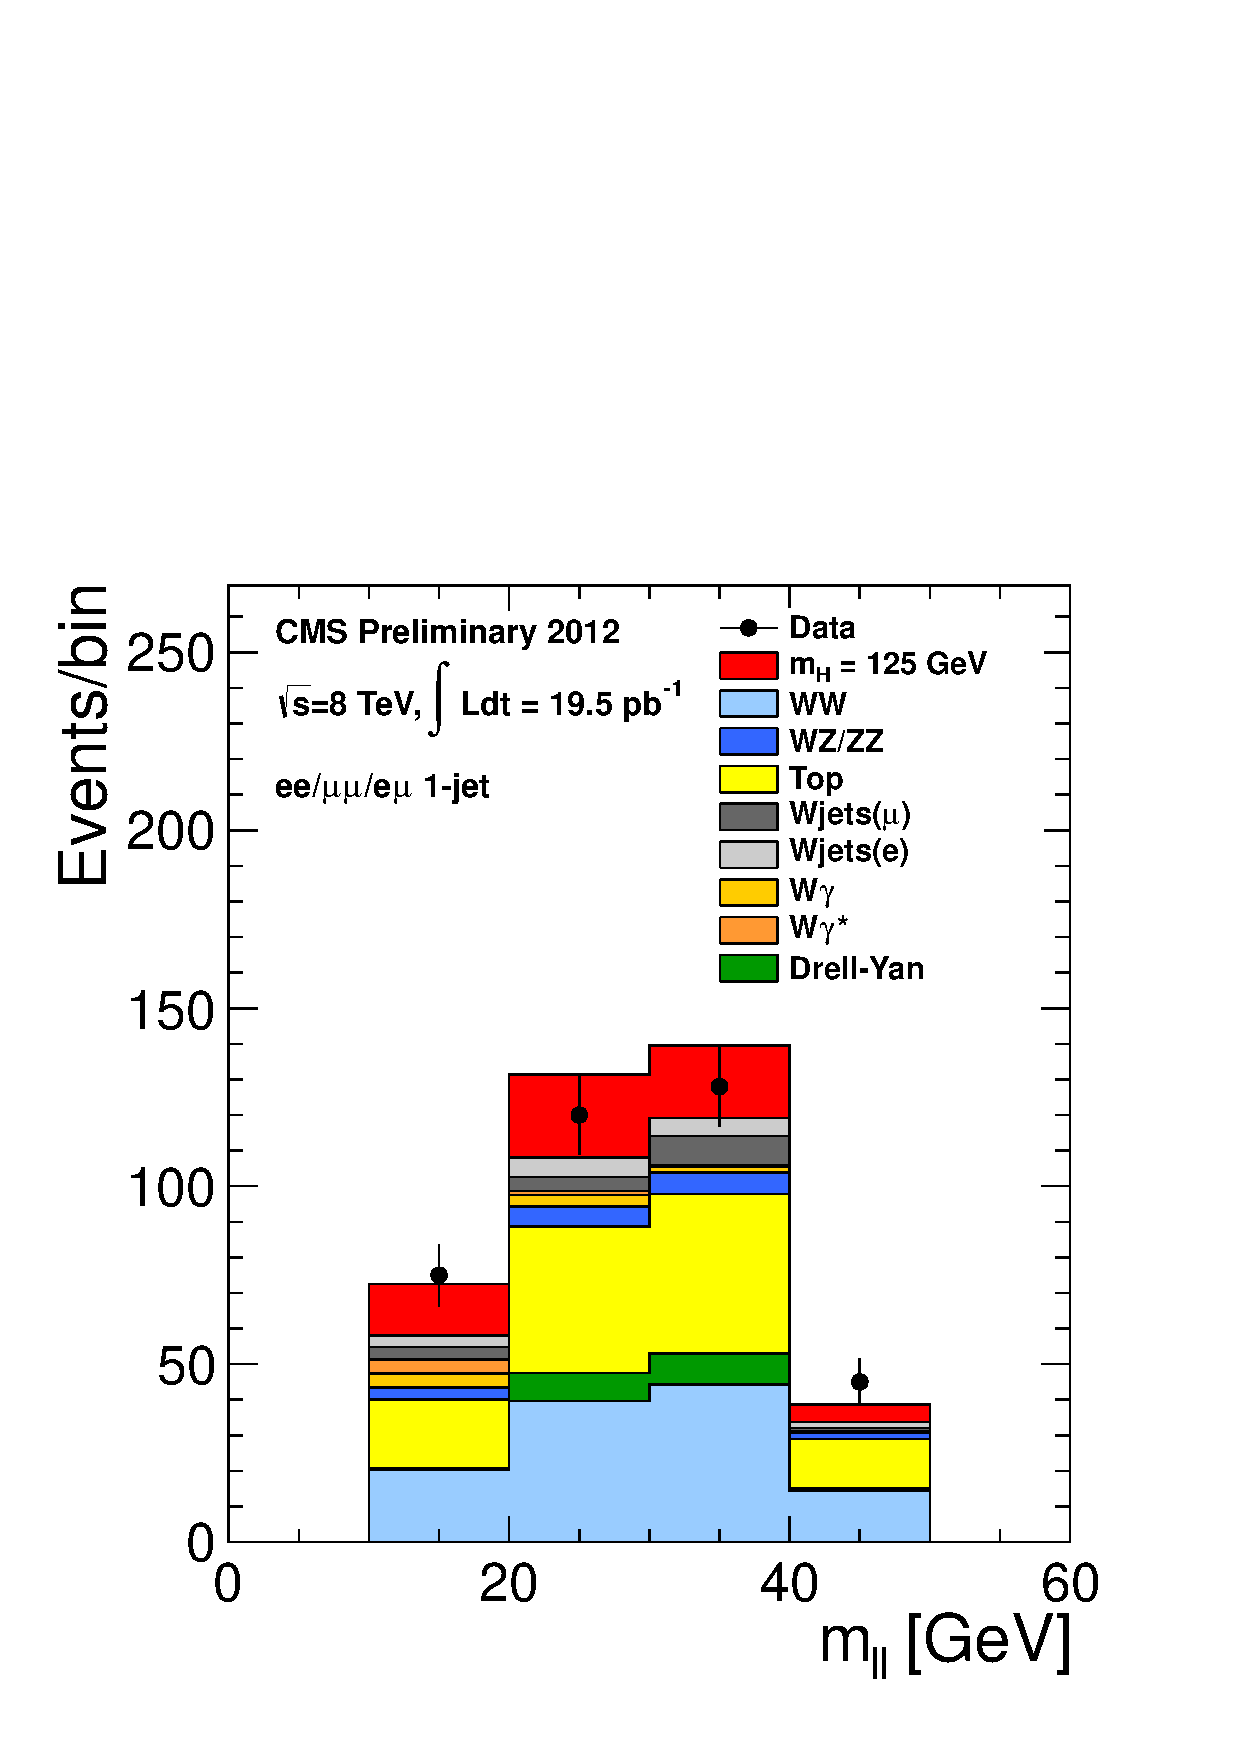
\includegraphics[width=0.45\textwidth]{figures/hww_analysis17_125_ALL_incl_1j_mll.pdf}
\end{tabular} 
\caption{ \mT(left) and \mll(right) distributionss for \mHi=125~\GeV\ analysis 
in 1-jet category. 
Top is for \DF, middle is for \SF, and the bottom is for the inclusive channel.  
The data shows good agreement bewteen prediction assmuing \mHi=125~\GeV\ Higgs boson.} 
\label{fig:cutbased125_1jet} 
\end{figure} 

% 7 TeV
\begin{sidewaystable}
{
 \tiny
  \begin{center}
   \begin{tabular}{l | c c | c c c c c c c c c c | c | c}
    \hline
     process & qqH & ggH & qqWW & ggWW & VV & Top & Zjets & WjetsE & Wgamma & Wg3l & Ztt & WjetsM & $\sum$Bkg & Data \\
      \hline 
      \multicolumn{15}{c}{\mHi = 124~\GeV} \\
      \hline 
      \DF\ 0-jet & $0.2\pm0.0$ & $17.8\pm3.9$ & $68.0\pm7.3$ & $3.3\pm1.1$ & $1.5\pm0.2$ & $3.9\pm0.9$ & $0.5\pm0.4$ & $6.5\pm2.5$ & $3.5\pm2.7$ & $2.9\pm1.3$ & $0.0\pm0.0$ & $4.2\pm1.8$ & $94.3\pm8.6$ & 99 \\ % of 0j
      \DF\ 1-jet & $0.7\pm0.1$ & $6.3\pm2.1$ & $18.1\pm3.2$ & $1.0\pm0.4$ & $1.7\pm0.2$ & $13.1\pm1.0$ & $0.6\pm0.4$ & $3.1\pm1.3$ & $1.0\pm1.0$ & $1.0\pm0.6$ & $0.0\pm0.0$ & $3.0\pm1.4$ & $42.7\pm4.1$ & 48 \\ % of 1j
      \SF\ 0-jet & $0.1\pm0.0$ & $8.1\pm1.8$ & $40.9\pm4.5$ & $1.7\pm0.5$ & $0.8\pm0.1$ & $1.8\pm0.5$ & $10.5\pm4.1$ & $2.0\pm0.8$ & $0.0\pm0.0$ & $0.9\pm0.5$ & $0.0\pm0.0$ & $1.1\pm0.7$ & $59.7\pm6.3$ & 60 \\ %sf 0j
      \SF\ 1-jet & $0.3\pm0.0$ & $2.3\pm0.8$ & $8.7\pm1.6$ & $0.6\pm0.2$ & $0.6\pm0.1$ & $5.7\pm0.5$ & $9.7\pm4.0$ & $0.6\pm0.3$ & $0.0\pm0.0$ & $0.3\pm0.3$ & $0.0\pm0.0$ & $0.1\pm0.4$ & $26.4\pm4.4$ & 29 \\ %sf 1j
    \hline 
      \multicolumn{15}{c}{\mHi = 160~\GeV} \\
    \hline  
    \DF\ 0-jet & $0.9\pm0.1$ & $73.4\pm16.0$ & $40.5\pm4.4$ & $4.4\pm1.4$ & $0.7\pm0.1$ & $4.1\pm1.0$ & $0.0\pm0.0$ & $1.3\pm0.6$ & $0.9\pm1.0$ & $0.3\pm0.2$ & $0.0\pm0.0$ & $1.2\pm0.8$ & $53.4\pm5.0$ & 59 \\
    \DF\ 1-jet & $4.0\pm0.4$ & $33.1\pm10.5$ & $16.7\pm3.0$ & $1.5\pm0.5$ & $1.0\pm0.1$ & $14.1\pm1.1$ & $0.1\pm0.0$ & $1.2\pm0.6$ & $0.0\pm0.0$ & $0.3\pm0.2$ & $0.0\pm0.0$ & $0.4\pm0.5$ & $35.3\pm3.3$ & 32 \\
    \SF\ 0-jet & $0.6\pm0.1$ & $59.3\pm12.9$ & $34.4\pm3.8$ & $3.2\pm1.0$ & $0.5\pm0.1$ & $3.3\pm0.8$ & $3.4\pm3.5$ & $0.4\pm0.3$ & $0.0\pm0.0$ & $0.6\pm0.4$ & $0.0\pm0.0$ & $0.1\pm0.4$ & $45.9\pm5.4$ & 50 \\
    \SF\ 1-jet & $2.8\pm0.3$ & $24.3\pm7.7$ & $12.0\pm2.2$ & $1.2\pm0.4$ & $0.5\pm0.1$ & $10.2\pm0.9$ & $9.0\pm3.8$ & $0.2\pm0.2$ & $0.0\pm0.0$ & $0.1\pm0.2$ & $0.0\pm0.0$ & $1.4\pm0.9$ & $34.7\pm4.6$ & 47 \\
    \hline 
      \multicolumn{15}{c}{\mHi = 200~\GeV} \\
    \hline  
    \DF\ 0-jet & $0.4\pm0.0$ & $28.3\pm6.4$ & $64.3\pm7.1$ & $7.1\pm2.2$ & $1.0\pm0.1$ & $11.1\pm2.5$ & $0.1\pm0.0$ & $2.5\pm1.1$ & $0.0\pm0.0$ & $0.1\pm0.2$ & $0.0\pm0.0$ & $0.3\pm0.5$ & $86.7\pm7.9$ & 85 \\
    \DF\ 1-jet & $2.3\pm0.2$ & $13.7\pm4.1$ & $28.7\pm5.2$ & $2.7\pm0.9$ & $1.1\pm0.1$ & $31.1\pm2.2$ & $0.2\pm0.0$ & $1.8\pm0.8$ & $0.0\pm0.0$ & $0.0\pm0.0$ & $0.0\pm0.0$ & $0.4\pm0.6$ & $66.0\pm5.8$ & 49 \\
    \SF\ 0-jet & $0.4\pm0.0$ & $24.0\pm5.4$ & $49.8\pm5.5$ & $5.8\pm1.8$ & $0.7\pm0.1$ & $6.9\pm1.6$ & $3.8\pm2.6$ & $0.7\pm0.2$ & $0.0\pm0.0$ & $0.0\pm0.0$ & $0.0\pm0.0$ & $0.6\pm0.7$ & $68.3\pm6.6$ & 70 \\
    \SF\ 1-jet & $1.5\pm0.2$ & $9.8\pm3.0$ & $20.2\pm3.7$ & $2.0\pm0.7$ & $0.7\pm0.1$ & $20.6\pm1.5$ & $15.2\pm5.1$ & $0.4\pm0.3$ & $0.0\pm0.0$ & $0.0\pm0.0$ & $0.0\pm0.0$ & $1.7\pm1.0$ & $60.9\pm6.6$ & 56 \\
    \hline
      \multicolumn{15}{c}{\mHi = 400~\GeV} \\
    \hline  
    \DF\ 0-jet & $0.2\pm0.0$ & $11.0\pm3.0$ & $34.6\pm3.8$ & $2.6\pm0.8$ & $0.9\pm0.1$ & $17.4\pm3.9$ & $0.1\pm0.0$ & $3.1\pm1.2$ & $0.0\pm0.0$ & $1.4\pm0.7$ & $0.0\pm0.0$ & $0.2\pm0.5$ & $60.2\pm5.7$ & 58 \\
    \DF\ 1-jet & $0.7\pm0.1$ & $7.6\pm2.3$ & $28.8\pm4.6$ & $1.5\pm0.5$ & $1.1\pm0.1$ & $34.2\pm2.4$ & $1.0\pm0.7$ & $3.5\pm1.4$ & $0.0\pm0.0$ & $0.3\pm0.3$ & $0.0\pm0.0$ & $0.8\pm0.7$ & $71.2\pm5.5$ & 60 \\
    \SF\ 0-jet & $0.1\pm0.0$ & $8.8\pm2.4$ & $25.6\pm2.9$ & $2.0\pm0.6$ & $0.5\pm0.1$ & $11.1\pm2.5$ & $3.0\pm0.3$ & $2.2\pm0.9$ & $0.0\pm0.0$ & $6.1\pm2.7$ & $0.0\pm0.0$ & $0.2\pm0.4$ & $50.8\pm4.8$ & 45 \\
    \SF\ 1-jet & $0.5\pm0.1$ & $5.3\pm1.6$ & $16.3\pm2.6$ & $0.9\pm0.3$ & $0.6\pm0.1$ & $19.8\pm1.4$ & $6.6\pm2.7$ & $1.6\pm0.7$ & $0.0\pm0.0$ & $1.6\pm0.8$ & $0.0\pm0.0$ & $0.1\pm0.4$ & $47.5\pm4.2$ & 65 \\
    \hline 
      \multicolumn{15}{c}{\mHi = 600~\GeV} \\
    \hline  
    \DF\ 0-jet & $0.1\pm0.0$ & $1.7\pm0.6$ & $10.1\pm1.2$ & $0.8\pm0.3$ & $0.2\pm0.0$ & $5.3\pm1.2$ & $0.0\pm0.0$ & $1.1\pm0.5$ & $0.0\pm0.0$ & $0.3\pm0.1$ & $0.0\pm0.0$ & $0.0\pm0.0$ & $17.9\pm1.8$ & 16 \\
    \DF\ 1-jet & $0.3\pm0.0$ & $1.5\pm0.5$ & $10.1\pm1.7$ & $0.5\pm0.2$ & $0.4\pm0.1$ & $9.8\pm0.8$ & $1.0\pm0.7$ & $1.7\pm0.7$ & $0.0\pm0.0$ & $0.2\pm0.2$ & $0.0\pm0.0$ & $0.6\pm0.5$ & $24.1\pm2.2$ & 19 \\
    \SF\ 0-jet & $0.1\pm0.0$ & $1.2\pm0.5$ & $5.5\pm0.7$ & $0.6\pm0.2$ & $0.2\pm0.0$ & $3.3\pm0.8$ & $1.0\pm0.1$ & $0.9\pm0.4$ & $0.0\pm0.0$ & $0.0\pm0.0$ & $0.0\pm0.0$ & $0.2\pm0.3$ & $11.6\pm1.2$ & 13 \\
    \SF\ 1-jet & $0.2\pm0.0$ & $1.0\pm0.3$ & $5.2\pm0.9$ & $0.3\pm0.1$ & $0.2\pm0.0$ & $4.9\pm0.5$ & $0.6\pm0.1$ & $0.9\pm0.4$ & $0.0\pm0.0$ & $0.3\pm0.3$ & $0.0\pm0.0$ & $0.1\pm0.3$ & $12.6\pm1.2$ & 16 \\
   \hline
   \end{tabular}
   \end{center}
    }
    \caption{Table of yields in cut-based analysis at 7~\TeV\ in \intlumiSevenTeV. 
    All final states are shown separately. Yields for each process 
    and the corresponding uncertainties(stats.+syst.) are shown. The last two 
    colunms show the sum of all backgrounds and the data counts. For 7 \TeV, \mHi=124~\GeV\ 
    is used instead of 125~\GeV because 125~\GeV\ sample does not exist. }
    \label{tab:cut7tev}
\end{sidewaystable}

% 8 TeV
\begin{sidewaystable}
{
 \tiny
  \begin{center}
   \begin{tabular}{l | c c | c c c c c c c c c c | c | c}
    \hline
     process & qqH & ggH & qqWW & ggWW & VV & Top & Zjets & WjetsE & Wgamma & Wg3l & Ztt & WjetsM & $\sum$Bkg & Data \\
      \hline 
      \multicolumn{15}{c}{\mHi = 124~\GeV} \\
      \hline 
    \DF\ 0-jet & $1.0\pm0.1$ & $88.9\pm19.3$ & $294.1\pm28.4$ & $16.0\pm5.0$ & $10.2\pm1.0$ & $20.0\pm4.3$ & $0.0\pm0.0$ & $26.4\pm9.6$ & $21.2\pm9.8$ & $18.3\pm8.1$ & $1.2\pm0.2$ & $21.4\pm8.0$ & $428.8\pm34.2$ & 505 \\
    \DF\ 1-jet & $4.6\pm0.5$ & $37.5\pm12.2$ & $74.5\pm10.4$ & $4.8\pm1.6$ & $10.2\pm1.1$ & $78.8\pm4.5$ & $0.0\pm0.0$ & $12.7\pm4.7$ & $6.8\pm4.0$ & $4.5\pm2.3$ & $2.7\pm0.4$ & $12.9\pm5.0$ & $208.0\pm14.1$ & 228 \\
    \SF\ 0-jet & $0.5\pm0.1$ & $55.8\pm12.2$ & $197.2\pm19.2$ & $9.7\pm3.1$ & $13.3\pm1.3$ & $9.3\pm2.2$ & $92.2\pm31.0$ & $12.1\pm4.5$ & $3.2\pm2.5$ & $6.1\pm2.9$ & $0.0\pm0.0$ & $16.5\pm6.2$ & $359.6\pm37.6$ & 421 \\
    \SF\ 1-jet & $2.1\pm0.2$ & $15.9\pm5.2$ & $37.5\pm5.3$ & $2.2\pm0.8$ & $6.5\pm1.0$ & $40.4\pm3.1$ & $14.7\pm5.3$ & $2.8\pm1.2$ & $2.5\pm1.5$ & $0.8\pm0.7$ & $0.0\pm0.0$ & $3.7\pm1.6$ & $111.0\pm8.6$ & 140 \\
    \hline 
      \multicolumn{15}{c}{\mHi = 160~\GeV} \\
    \hline  
    \DF\ 0-jet & $6.2\pm0.6$ & $371.6\pm81.1$ & $175.6\pm17.1$ & $20.7\pm6.5$ & $5.8\pm0.6$ & $24.9\pm5.5$ & $0.0\pm0.0$ & $4.7\pm1.8$ & $4.6\pm3.3$ & $1.7\pm1.1$ & $0.1\pm0.1$ & $1.1\pm0.9$ & $239.3\pm19.5$ & 285 \\
    \DF\ 1-jet & $24.4\pm2.6$ & $181.2\pm57.6$ & $66.1\pm9.3$ & $6.6\pm2.2$ & $7.5\pm0.9$ & $82.9\pm4.7$ & $0.0\pm0.0$ & $6.4\pm2.4$ & $0.2\pm0.2$ & $0.9\pm0.7$ & $0.5\pm0.2$ & $2.3\pm1.4$ & $173.3\pm11.0$ & 226 \\
    \SF\ 0-jet & $4.7\pm0.5$ & $321.2\pm70.1$ & $148.4\pm14.5$ & $15.9\pm5.0$ & $9.7\pm1.0$ & $14.0\pm3.2$ & $18.8\pm9.7$ & $2.5\pm1.1$ & $1.0\pm0.7$ & $0.8\pm0.5$ & $0.0\pm0.0$ & $3.2\pm1.5$ & $214.3\pm18.6$ & 256 \\
    \SF\ 1-jet & $13.7\pm1.5$ & $103.6\pm33.0$ & $42.6\pm6.1$ & $3.7\pm1.3$ & $5.4\pm0.8$ & $47.6\pm3.2$ & $8.8\pm4.0$ & $1.4\pm0.7$ & $1.3\pm1.0$ & $0.0\pm0.0$ & $0.0\pm0.0$ & $2.7\pm1.4$ & $113.6\pm8.3$ & 134 \\
    \hline 
      \multicolumn{15}{c}{\mHi = 200~\GeV} \\
    \hline  
    \DF\ 0-jet & $3.1\pm0.3$ & $150.5\pm34.1$ & $286.2\pm27.8$ & $32.3\pm10.0$ & $10.1\pm1.1$ & $54.6\pm11.2$ & $0.0\pm0.0$ & $5.7\pm2.2$ & $2.1\pm2.2$ & $1.7\pm1.3$ & $0.6\pm0.2$ & $1.3\pm1.0$ & $394.6\pm31.8$ & 471 \\
    \DF\ 1-jet & $13.1\pm1.4$ & $78.1\pm23.7$ & $117.5\pm16.5$ & $11.1\pm3.7$ & $10.4\pm1.2$ & $187.0\pm8.3$ & $0.0\pm0.0$ & $9.4\pm3.5$ & $2.6\pm2.4$ & $0.3\pm0.3$ & $1.4\pm0.3$ & $4.3\pm2.0$ & $344.0\pm19.4$ & 421 \\
    \SF\ 0-jet & $2.6\pm0.3$ & $120.5\pm27.3$ & $230.9\pm22.5$ & $29.0\pm9.0$ & $19.5\pm1.9$ & $41.8\pm8.7$ & $20.1\pm7.7$ & $4.5\pm1.8$ & $1.8\pm1.1$ & $1.1\pm0.8$ & $0.0\pm0.0$ & $2.5\pm1.4$ & $351.1\pm27.1$ & 390 \\
    \SF\ 1-jet & $7.4\pm0.8$ & $47.9\pm14.6$ & $77.6\pm11.0$ & $7.4\pm2.5$ & $11.1\pm1.5$ & $120.1\pm6.2$ & $16.6\pm5.7$ & $2.7\pm1.1$ & $0.0\pm 0.0$ & $0.0\pm0.0$ & $0.0\pm0.0$ & $3.5\pm1.7$ & $239.0\pm 0.0$ & 261 \\
    \hline
      \multicolumn{15}{c}{\mHi = 400~\GeV} \\
    \hline  
    \DF\ 0-jet & $1.2\pm0.1$ & $63.0\pm17.3$ & $195.6\pm23.6$ & $14.0\pm4.5$ & $9.7\pm1.1$ & $91.9\pm18.3$ & $0.0\pm0.0$ & $9.4\pm3.6$ & $2.5\pm2.6$ & $2.7\pm1.7$ & $0.2\pm0.1$ & $0.0\pm0.0$ & $326.2\pm30.6$ & 306 \\
    \DF\ 1-jet & $4.4\pm0.5$ & $42.5\pm12.9$ & $125.1\pm19.7$ & $7.1\pm2.4$ & $10.9\pm1.2$ & $212.6\pm9.0$ & $0.0\pm0.0$ & $14.4\pm5.3$ & $0.4\pm0.4$ & $1.0\pm0.8$ & $2.0\pm0.4$ & $3.2\pm1.6$ & $376.7\pm22.5$ & 361 \\
    \SF\ 0-jet & $1.0\pm0.1$ & $53.9\pm14.8$ & $171.5\pm20.8$ & $10.8\pm3.5$ & $21.3\pm2.1$ & $71.8\pm14.4$ & $30.2\pm23.4$ & $7.4\pm2.8$ & $0.5\pm0.5$ & $0.8\pm0.7$ & $0.0\pm0.0$ & $0.0\pm0.0$ & $314.2\pm34.8$ & 290 \\
    \SF\ 1-jet & $3.0\pm0.3$ & $29.7\pm9.0$ & $69.8\pm11.1$ & $4.1\pm1.4$ & $11.4\pm1.3$ & $122.3\pm6.0$ & $21.2\pm16.5$ & $3.3\pm1.4$ & $0.0\pm 0.0$ & $1.1\pm0.9$ & $0.0\pm0.0$ & $2.1\pm1.2$ & $235.3\pm 0.0$ & 215 \\
    \hline 
      \multicolumn{15}{c}{\mHi = 600~\GeV} \\
    \hline  
    \DF\ 0-jet & $0.6\pm0.1$ & $10.1\pm3.7$ & $61.2\pm7.6$ & $5.1\pm1.7$ & $4.0\pm0.5$ & $30.0\pm6.4$ & $0.0\pm0.0$ & $3.4\pm1.4$ & $2.6\pm2.6$ & $1.3\pm0.9$ & $0.1\pm0.1$ & $0.0\pm0.0$ & $107.7\pm10.6$ & 95 \\
    \DF\ 1-jet & $2.1\pm0.2$ & $8.9\pm2.8$ & $47.1\pm7.5$ & $2.6\pm0.9$ & $4.7\pm0.6$ & $65.0\pm4.1$ & $0.0\pm0.0$ & $7.6\pm2.9$ & $0.0\pm 0.0$ & $0.4\pm0.5$ & $0.8\pm0.2$ & $1.5\pm0.9$ & $129.7\pm 0.0$ & 110 \\
    \SF\ 0-jet & $0.5\pm0.1$ & $8.8\pm3.2$ & $55.7\pm6.9$ & $4.4\pm1.5$ & $7.5\pm0.8$ & $21.9\pm4.8$ & $0.0\pm0.0$ & $2.7\pm1.2$ & $0.5\pm0.5$ & $0.0\pm0.0$ & $0.0\pm0.0$ & $0.0\pm0.0$ & $92.8\pm8.7$ & 94 \\
    \SF\ 1-jet & $1.3\pm0.1$ & $5.7\pm1.8$ & $24.6\pm4.0$ & $1.7\pm0.6$ & $4.2\pm0.6$ & $30.9\pm2.2$ & $0.0\pm0.0$ & $1.6\pm0.7$ & $0.0\pm 0.0$ & $0.0\pm0.0$ & $0.0\pm0.0$ & $0.2\pm0.4$ & $63.2\pm 0.0$ & 63 \\
   \hline
   \end{tabular}
   \end{center}
    }
    \caption{Table of yields in cut-based analysis at 8~\TeV\ in \intlumiEightTeV. 
    All final states are shown separately. Yields for each process 
    and the corresponding uncertainties(stats.+syst.) are shown. The last two 
    colunms show the sum of all backgrounds and the data counts. For 7 \TeV, \mHi=124~\GeV\ 
    is used instead of 125~\GeV because 125~\GeV\ sample does not exist. }
    \label{tab:cut8tev}
\end{sidewaystable}


\section{Shape-based method results}  

Figure~\ref{fig:post2D} shows the 2-dimensional templates of the post-fit signal
and the data subtracted by the post-fit backgrounds in the 0-jet and 1-jet categories. 
The plots show only the region where signal is 
populated($60<\mt<120~\GeV$ and $12<\mll<100~\GeV$).  
The data - background plots in 0-jet show good agreement with the \mHi=125~\GeV\
plot. The 1-jet plot do not have enough data to draw any conclusions.  

Figure~\ref{fig:post1Dprojection_1dweight} shows the stacked and data - backgrounds  
\mT(top) and \mll(bottom) distributions using the post-fit results of 
shape-based method in \DF\ final states combining 7 and 8~\TeV.
Before projected to \mll\ and \mT\, each bin of 2-dimensional templates 
is weighted by $\frac{S}{S+B}$ using the variable which is not plotted. 
Mathematically, when projecting to x axis,
the weight applied to each 2-dimensional bin is defined as 
\begin{eqnarray} 
w_{ij} 
= 
\frac{\displaystyle \sum_{i=1}^{N_{bin}} s_{ij}}
     {\displaystyle \sum_{i=1}^{N_{bin}} s_{ij} + b_{ij}}.   
\end{eqnarray}
Because the bins are summed in the x direction, 
the x information is not used when constructing the weight. 
So, if x and y variables are independent, the projected 
distribution is not biased by the weight.  
This is the case of \mll\ and \mT, which are weakly correlated.
Therefore, the projected \mll\ and \mT\ plots are 
unbiased by the weight.
After applying the weight, the plots are normalized such that 
the signal yield is same with the one before applying the weight.
The hatched area is the post-fit background uncertainty 
estimated by toys generated using the post-fit nuisance parameters.  
The data - backgrounds plots show a clear excess on top of backgrounds 
and a good agreement with \mHi=125~\GeV\ 
hypothesis in terms of normalization and shape. 


% 2D
\begin{figure}[htp] 
\centering 
\begin{tabular}{c} 
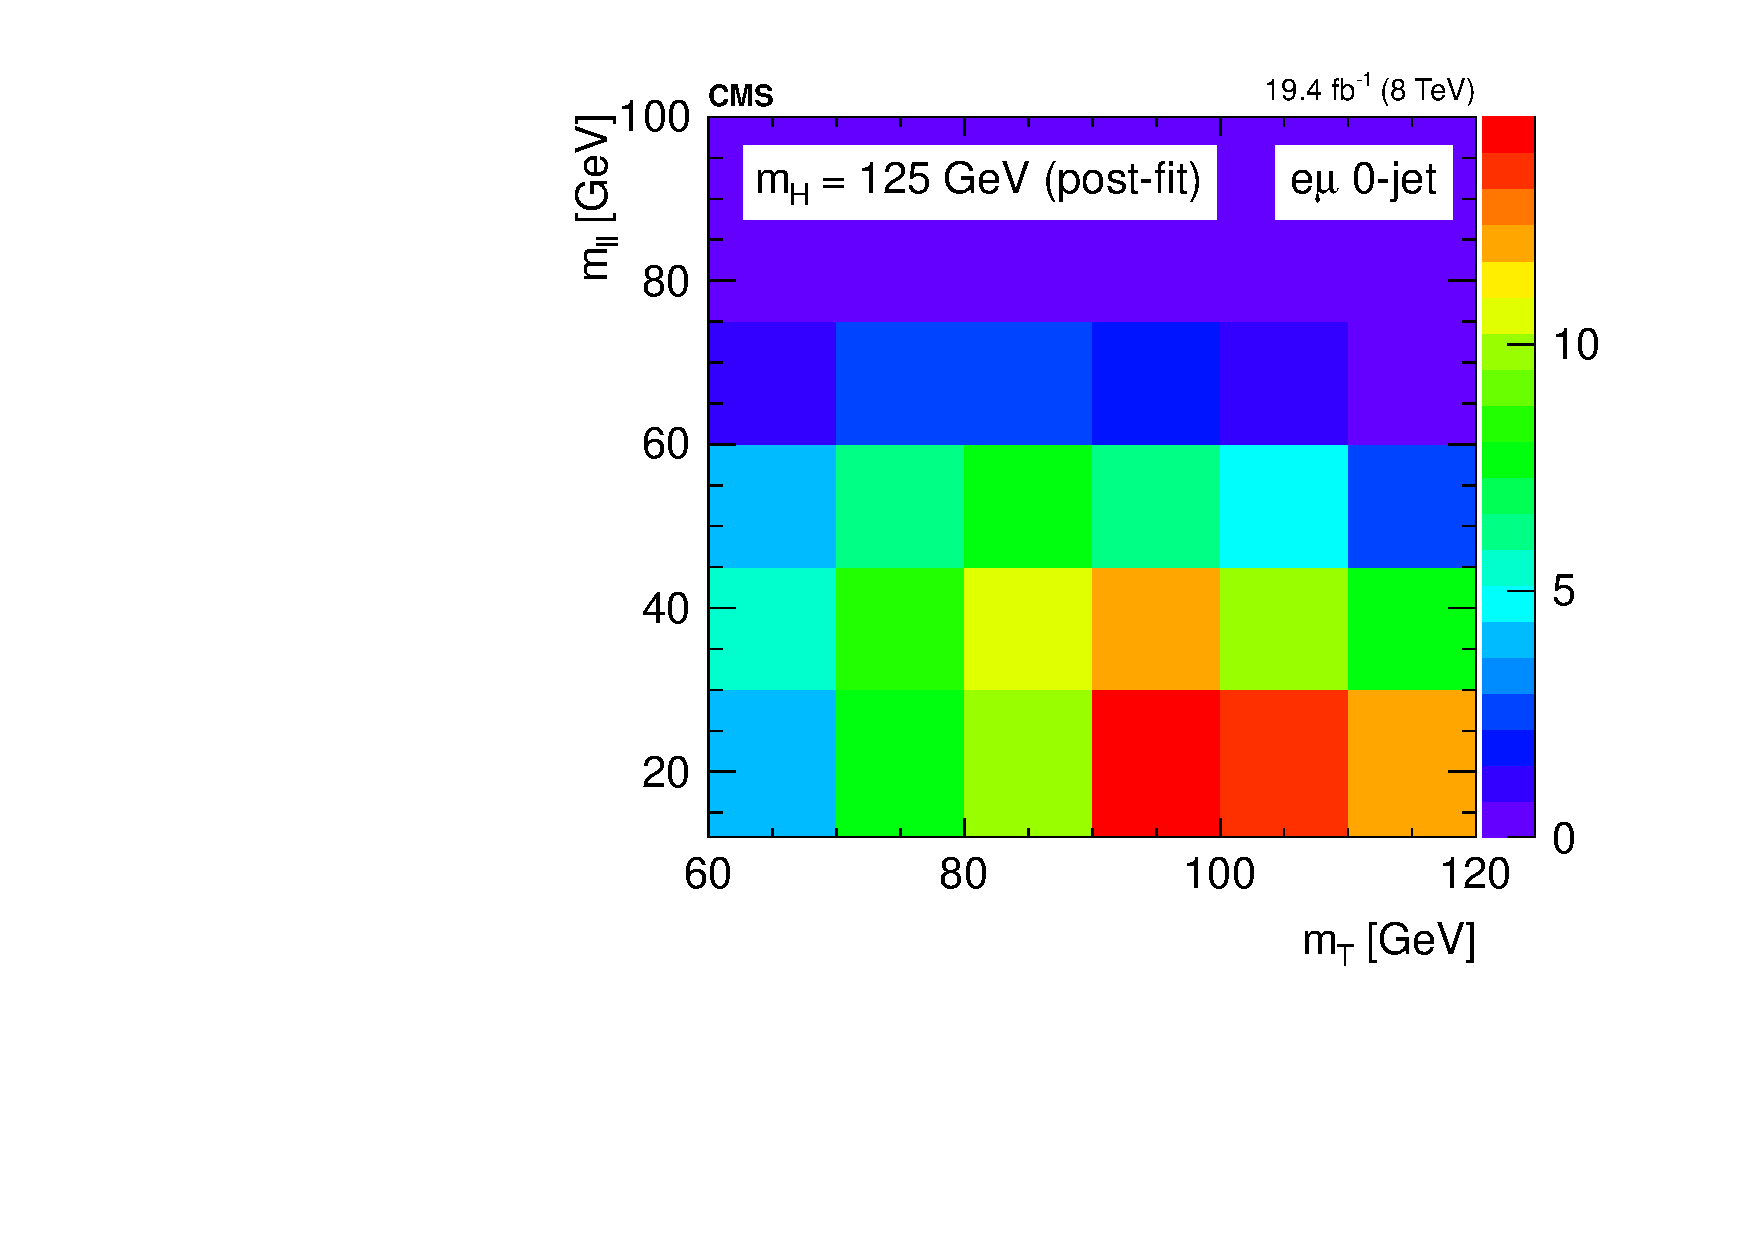
\includegraphics[width=0.45\textwidth]{figures/2d_postfit_0j_125_sig_paper.pdf}          
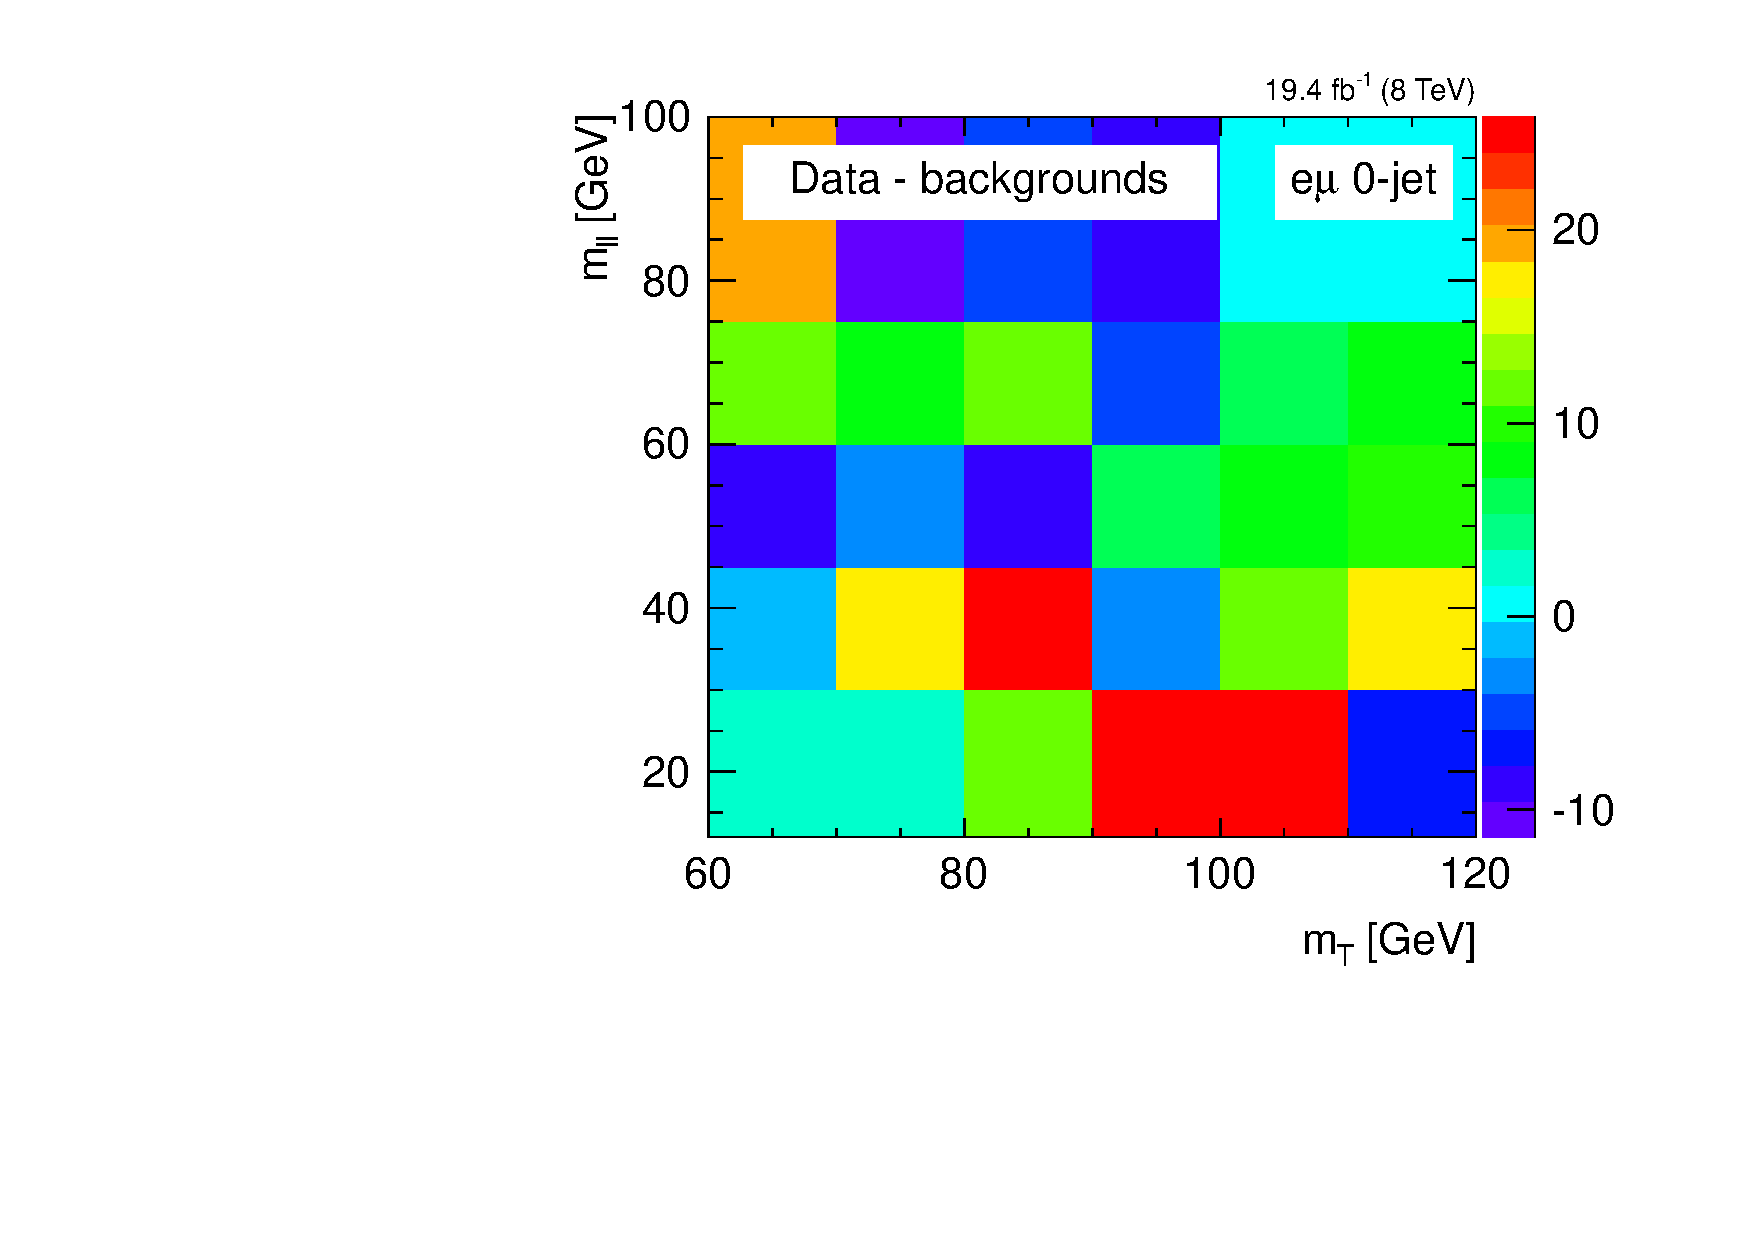
\includegraphics[width=0.45\textwidth]{figures/2d_postfit_0j_125_dataminusbkg_paper.pdf}          
\\
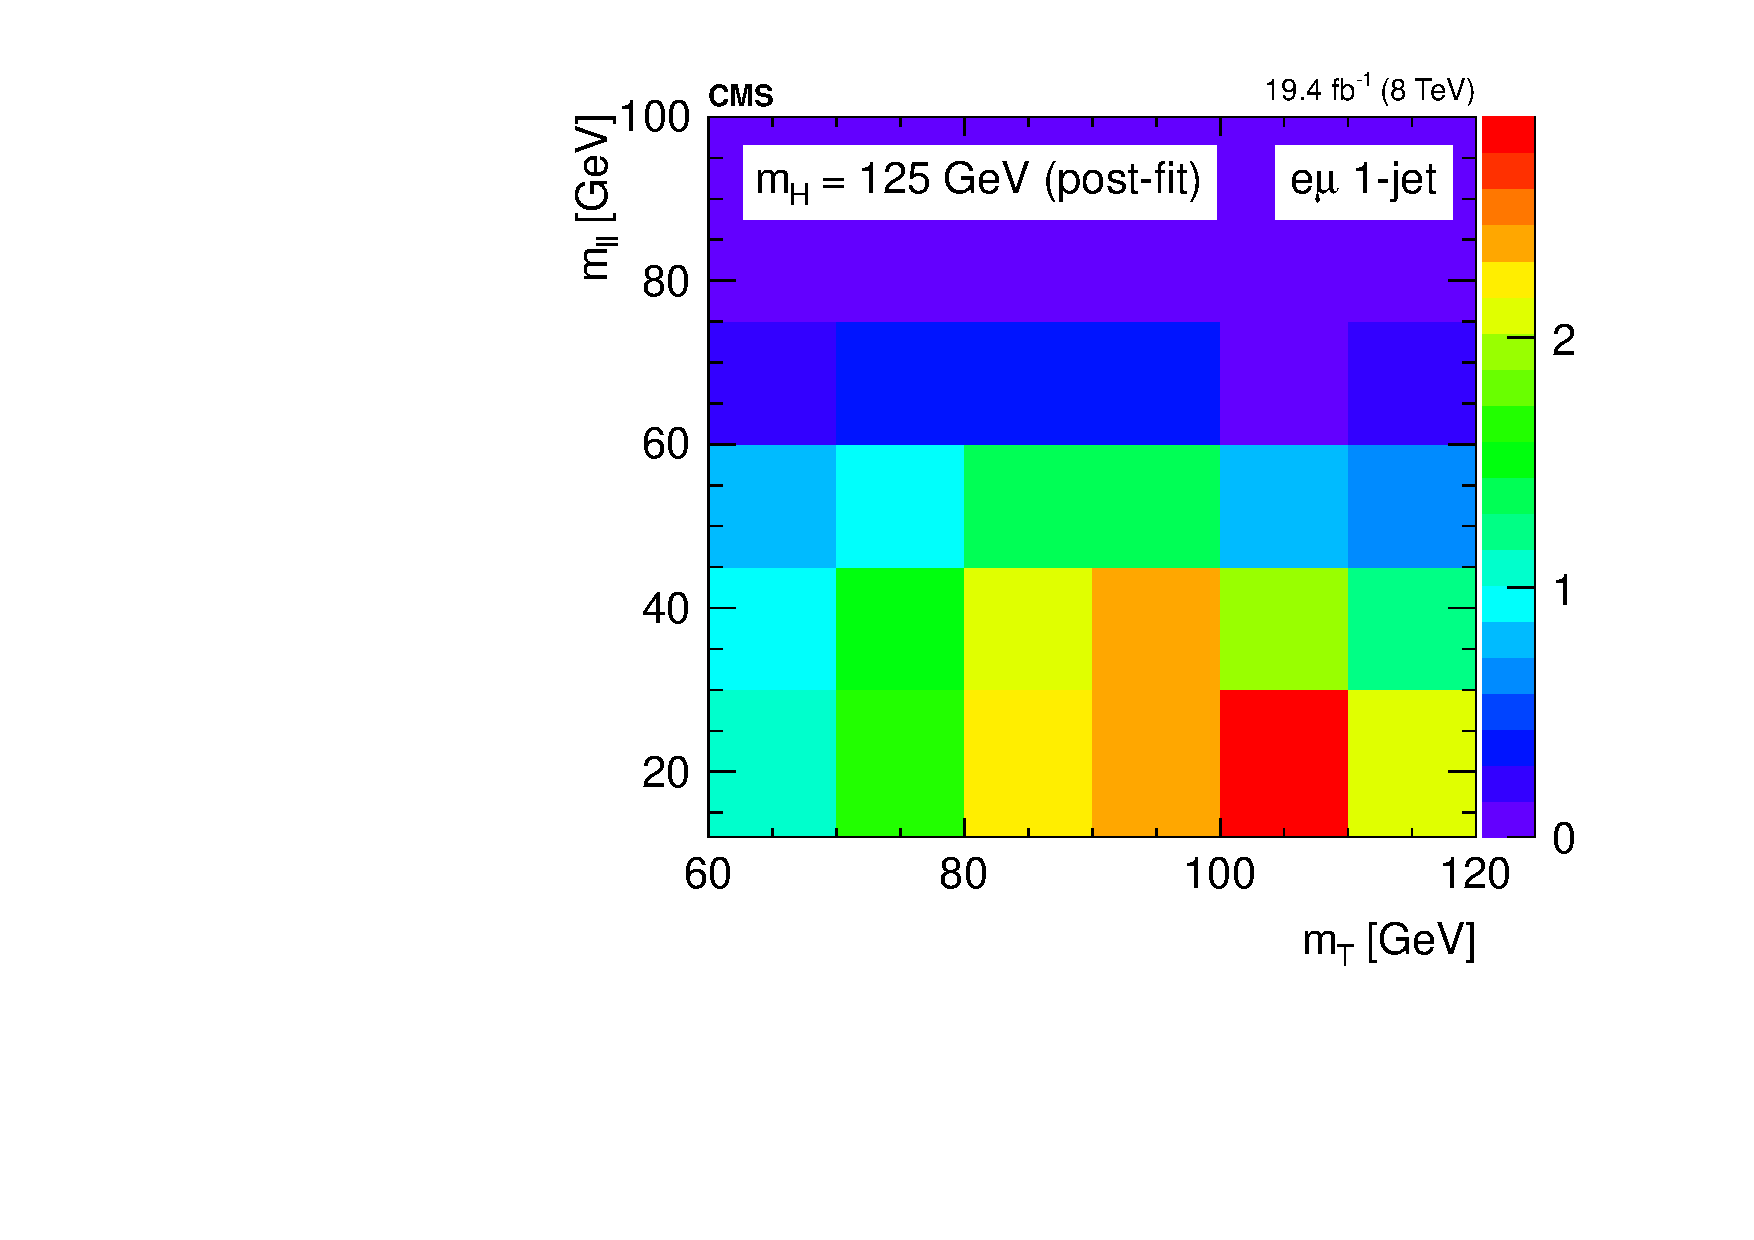
\includegraphics[width=0.45\textwidth]{figures/2d_postfit_1j_125_sig_paper.pdf}          
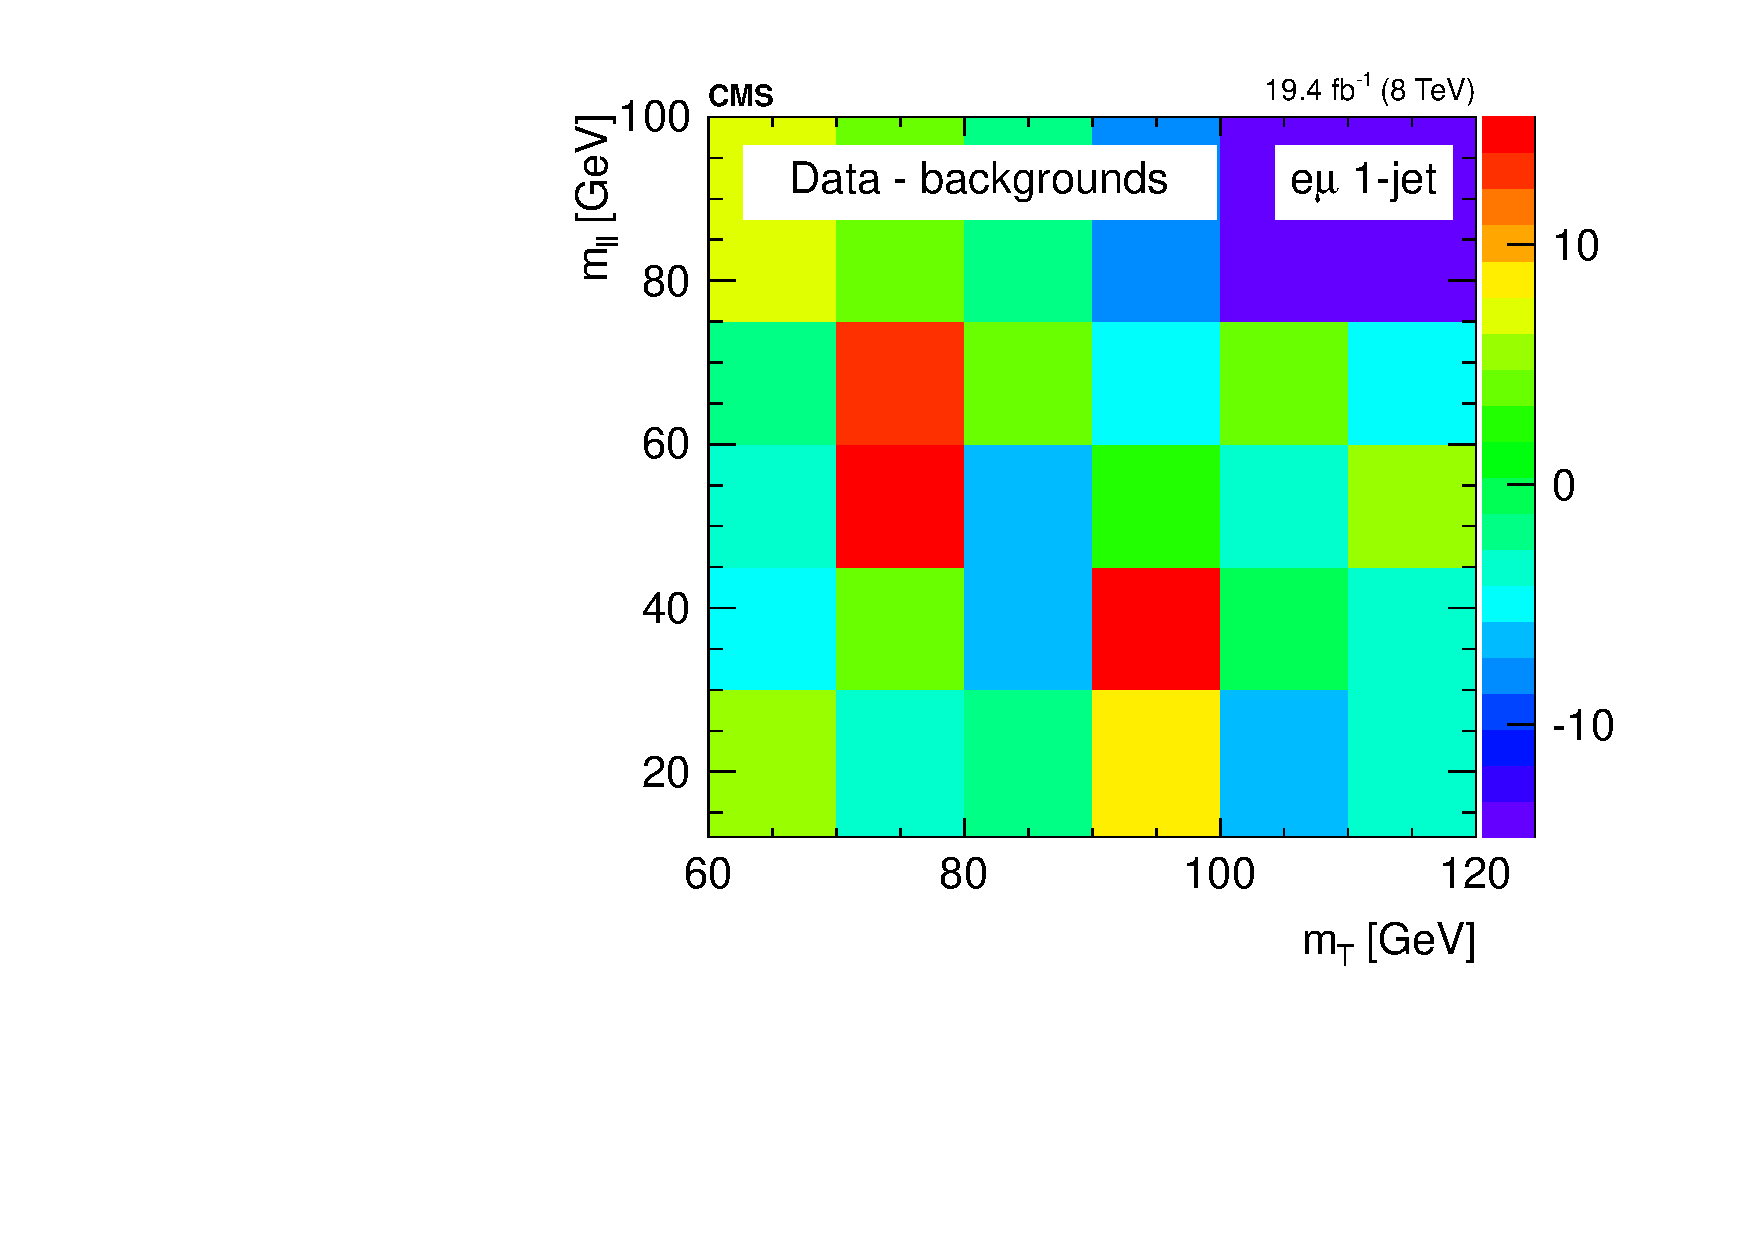
\includegraphics[width=0.45\textwidth]{figures/2d_postfit_1j_125_dataminusbkg_paper.pdf}          
\end{tabular} 
\caption{2D templates of post-fit signal(lest) and data subtracted by post backgrounds(right). 
The plots show only signal region defined by $60<\mt<120~\GeV$ and $12<\mll<100~\GeV$.
In 0-jet category(top) signal and data show a good agreement.  
In 1-jet category(top), data is not enough to draw a definitive conclusion. }
\label{fig:post2D} 
\end{figure} 


% 1D projection : 1D weight 
\begin{figure}[htp] 
\centering 
\begin{tabular}{c} 
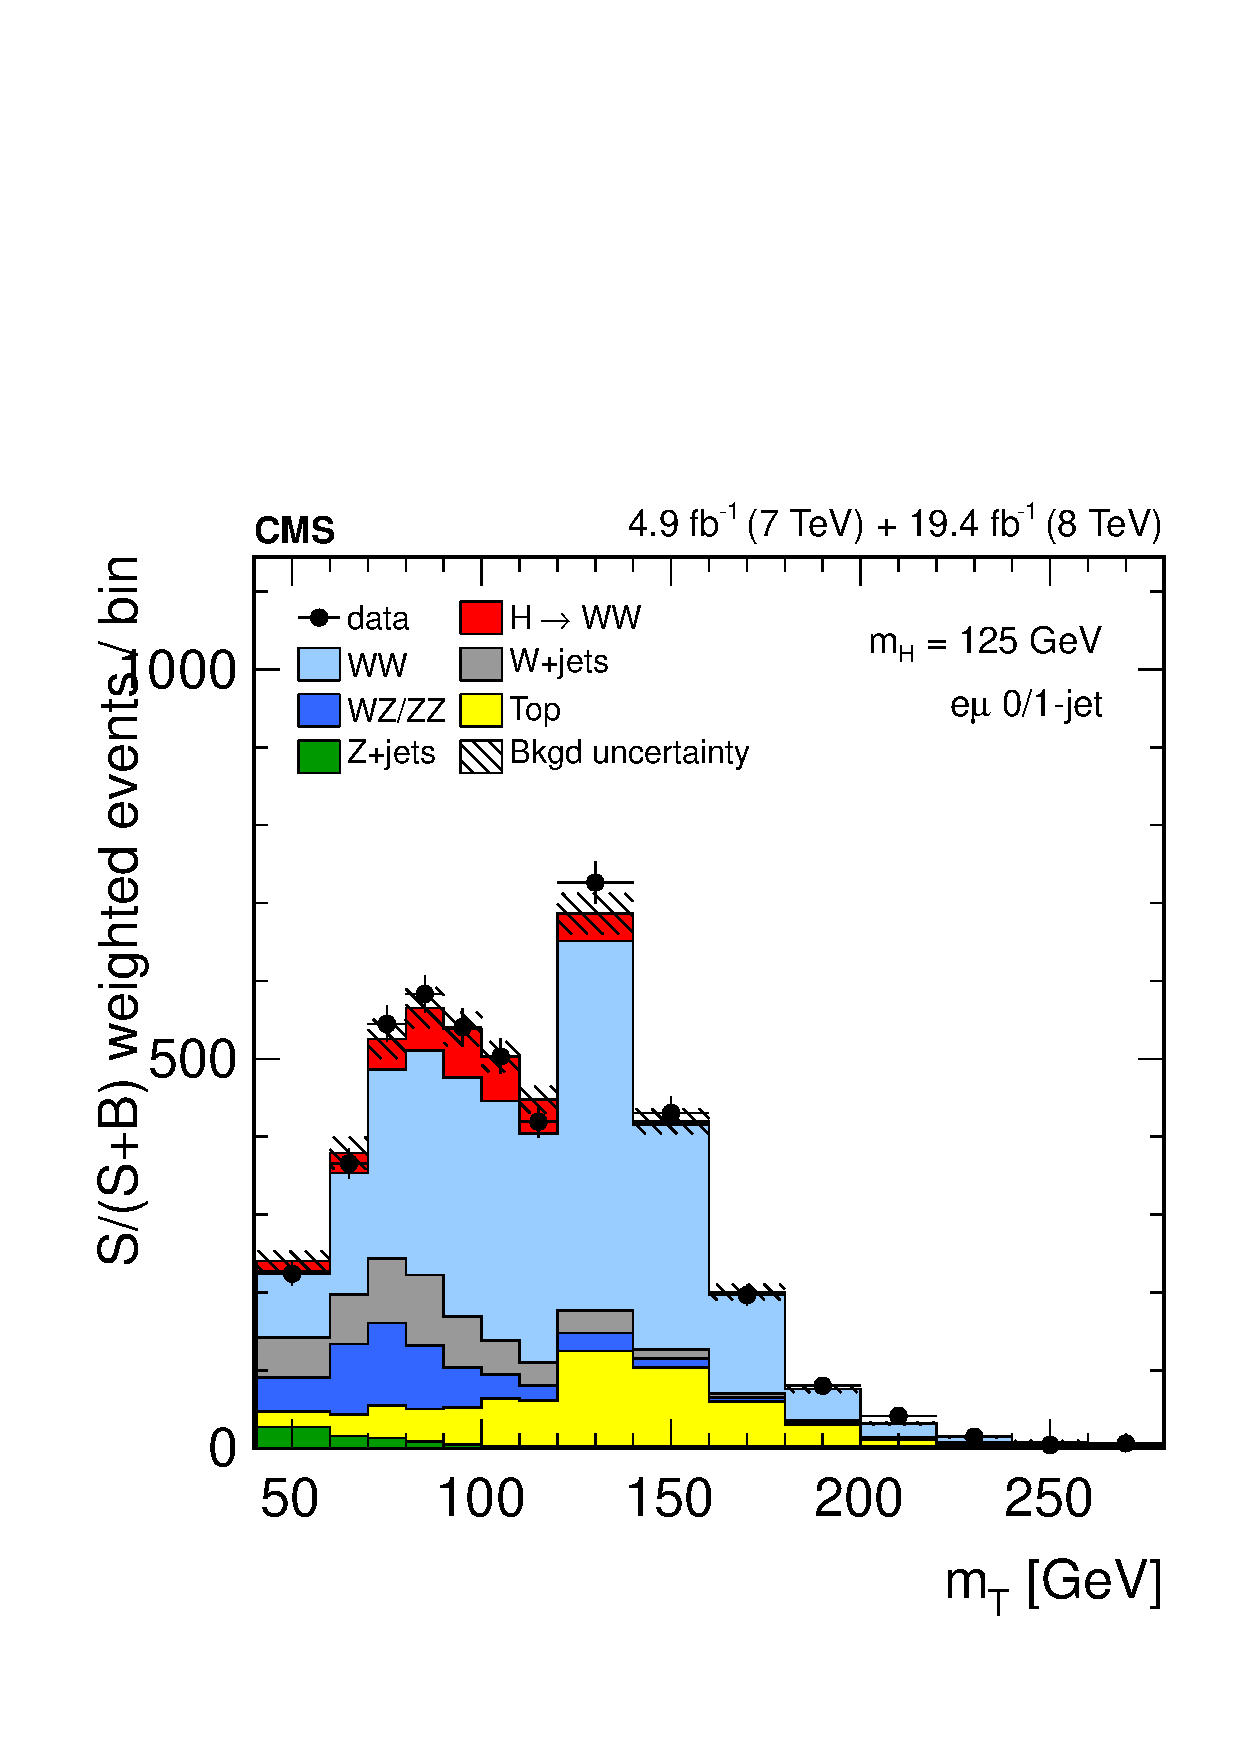
\includegraphics[width=0.49\textwidth]{figures/st_mT_1dweight.pdf}
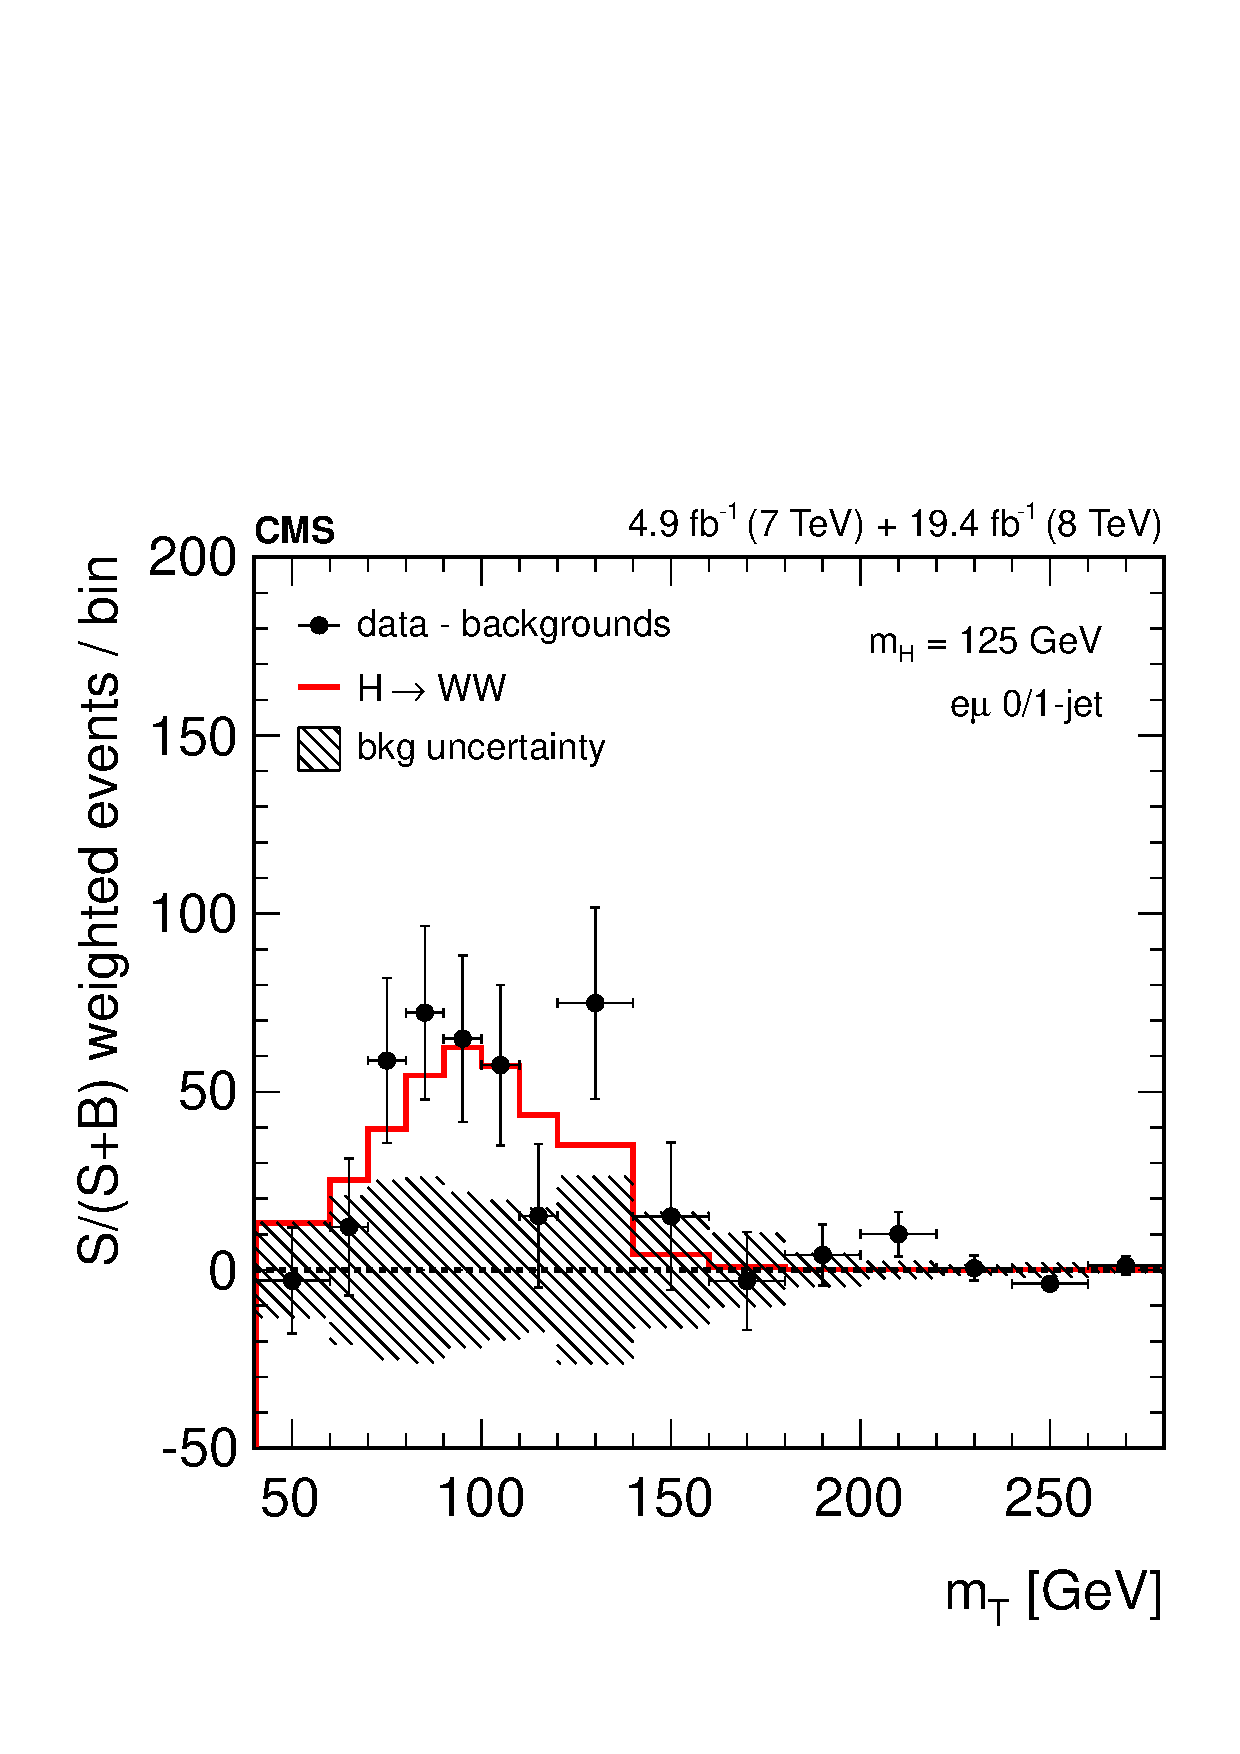
\includegraphics[width=0.49\textwidth]{figures/dataminusbkg_mT_1dweight.pdf} 
\\
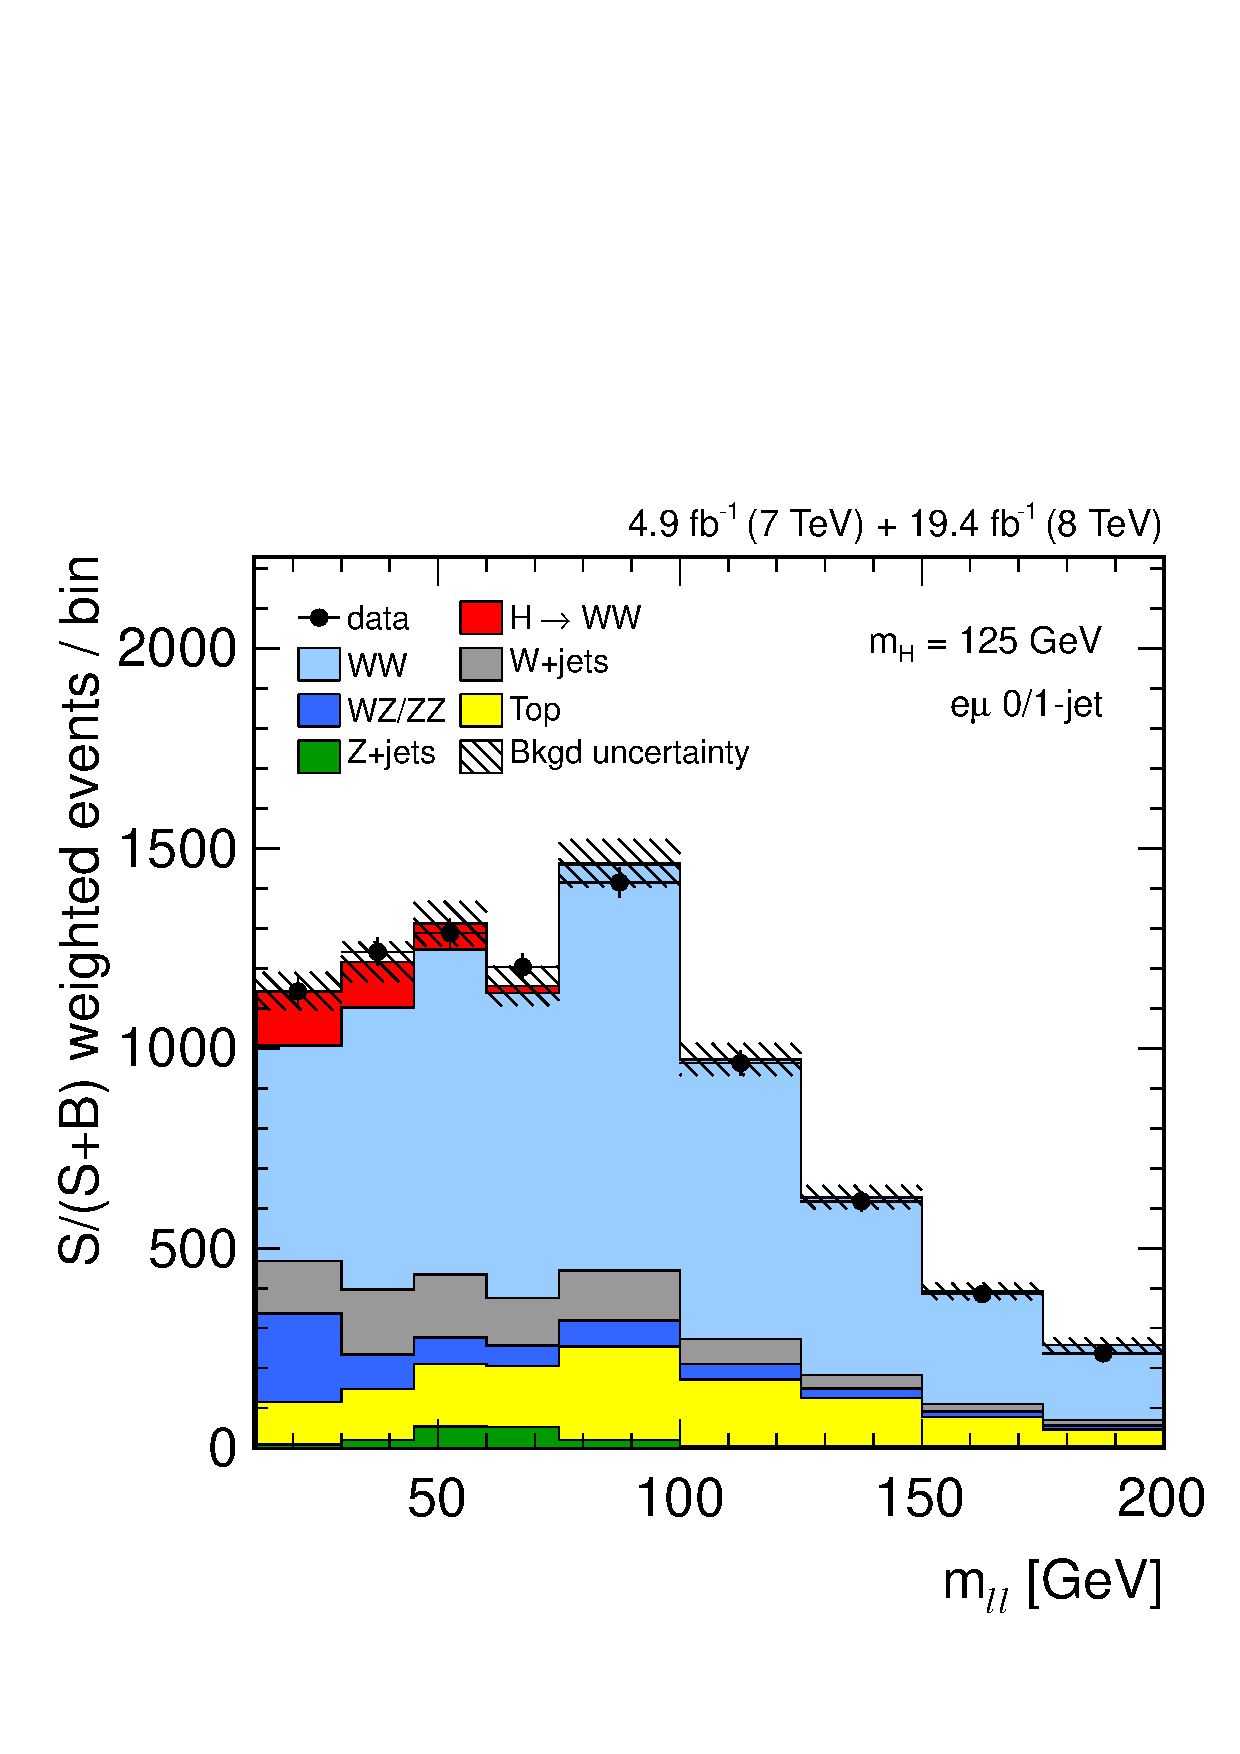
\includegraphics[width=0.49\textwidth]{figures/st_mll_1dweight.pdf}
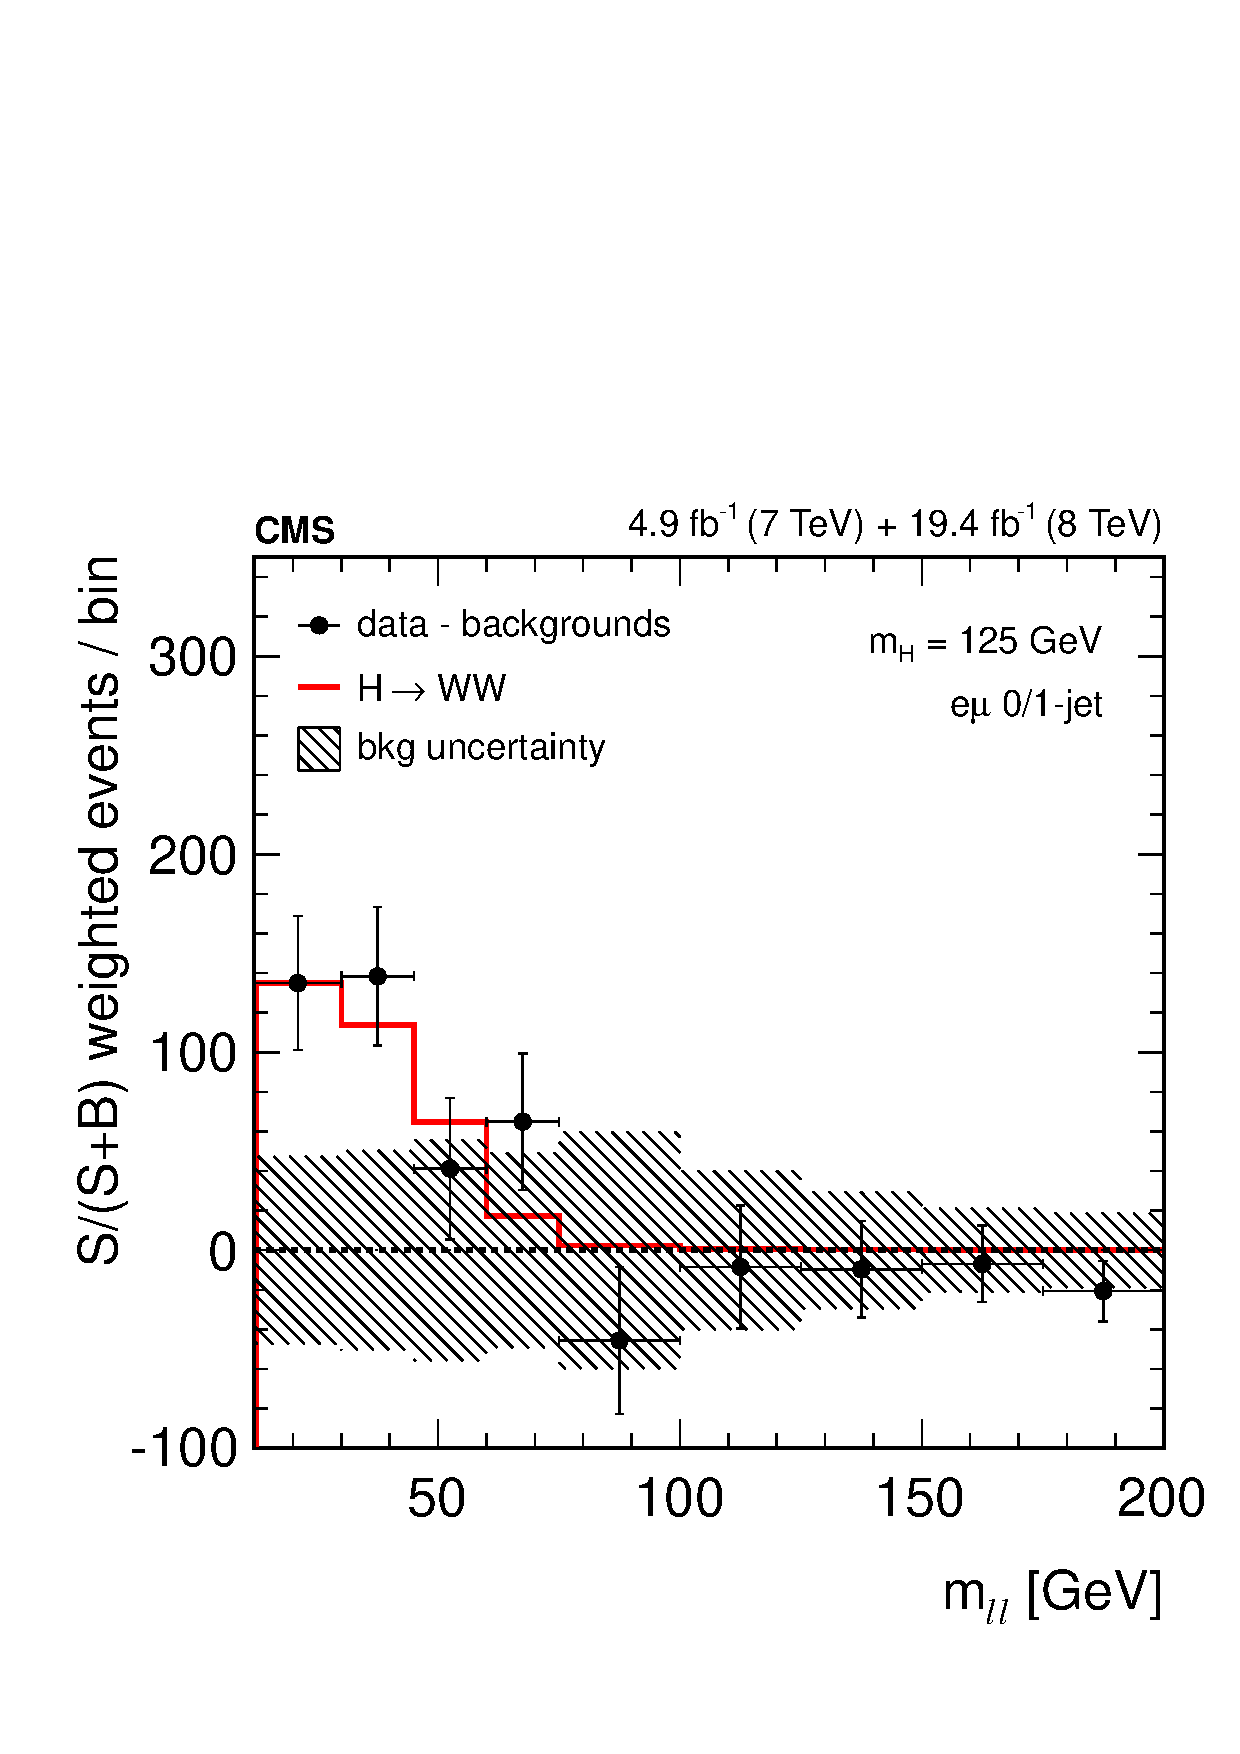
\includegraphics[width=0.49\textwidth]{figures/dataminusbkg_mll_1dweight.pdf} 
\end{tabular} 
\caption{Stacked and data - backgrounds 
\mT(top) and \mll(bottom) distributions using post-fit results 
of shape-based analysis
in \DF\ final states combining 7 and 8~\TeV.
In order to give more weights to sensitivie categories, each bin of 2D 
template is weighted by S/(S+B) and the total yield is normalized using the signal yield. 
Both normalization and shape of data show a very good agreement with SM Higgs at 125~\GeV.
The uncertainty is post-fit uncertainty.} 
\label{fig:post1Dprojection_1dweight} 
\end{figure} 

% 1D projection : 2D weight 
%\begin{figure}[htp] 
%\centering 
%\begin{tabular}{c} 
%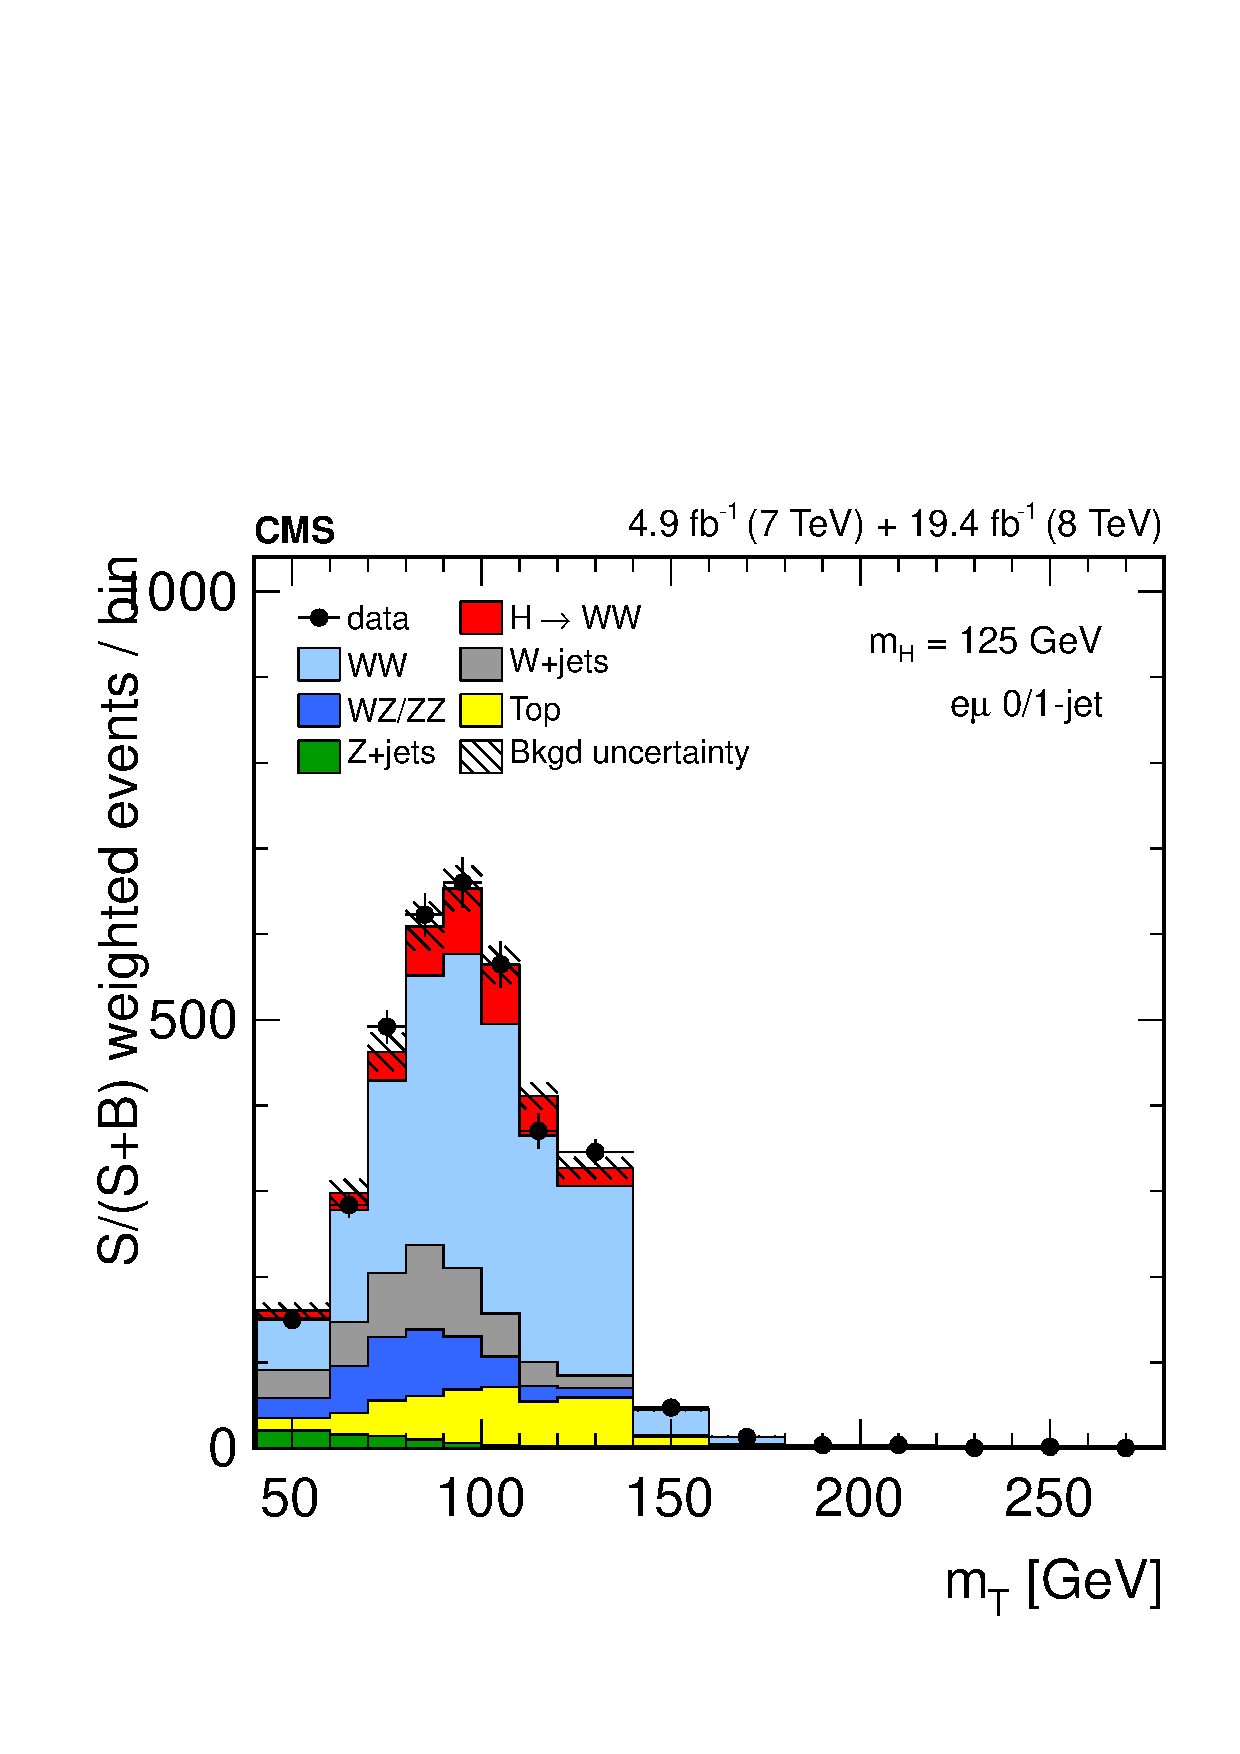
\includegraphics[width=0.49\textwidth]{figures/st_mT_2dweight.pdf}
%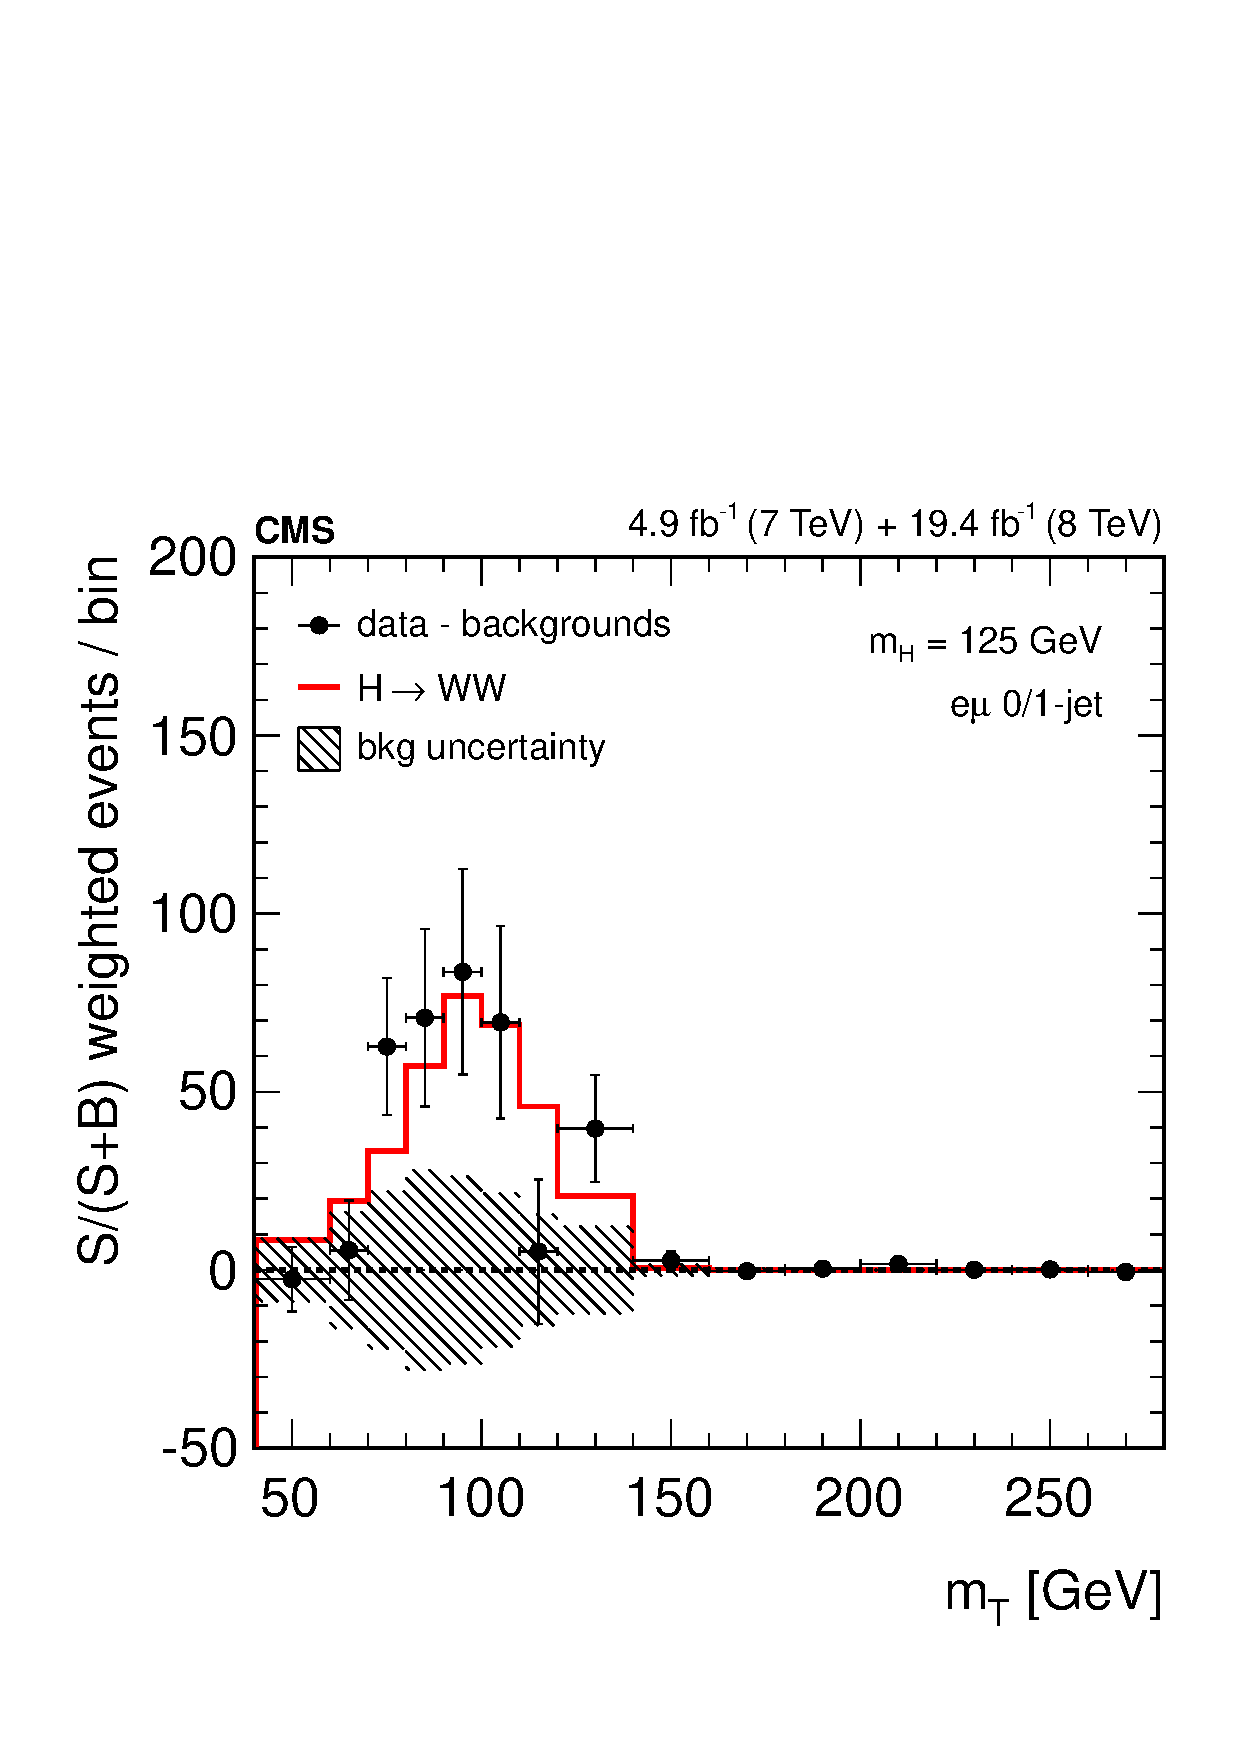
\includegraphics[width=0.49\textwidth]{figures/dataminusbkg_mT_2dweight.pdf} 
%\\
%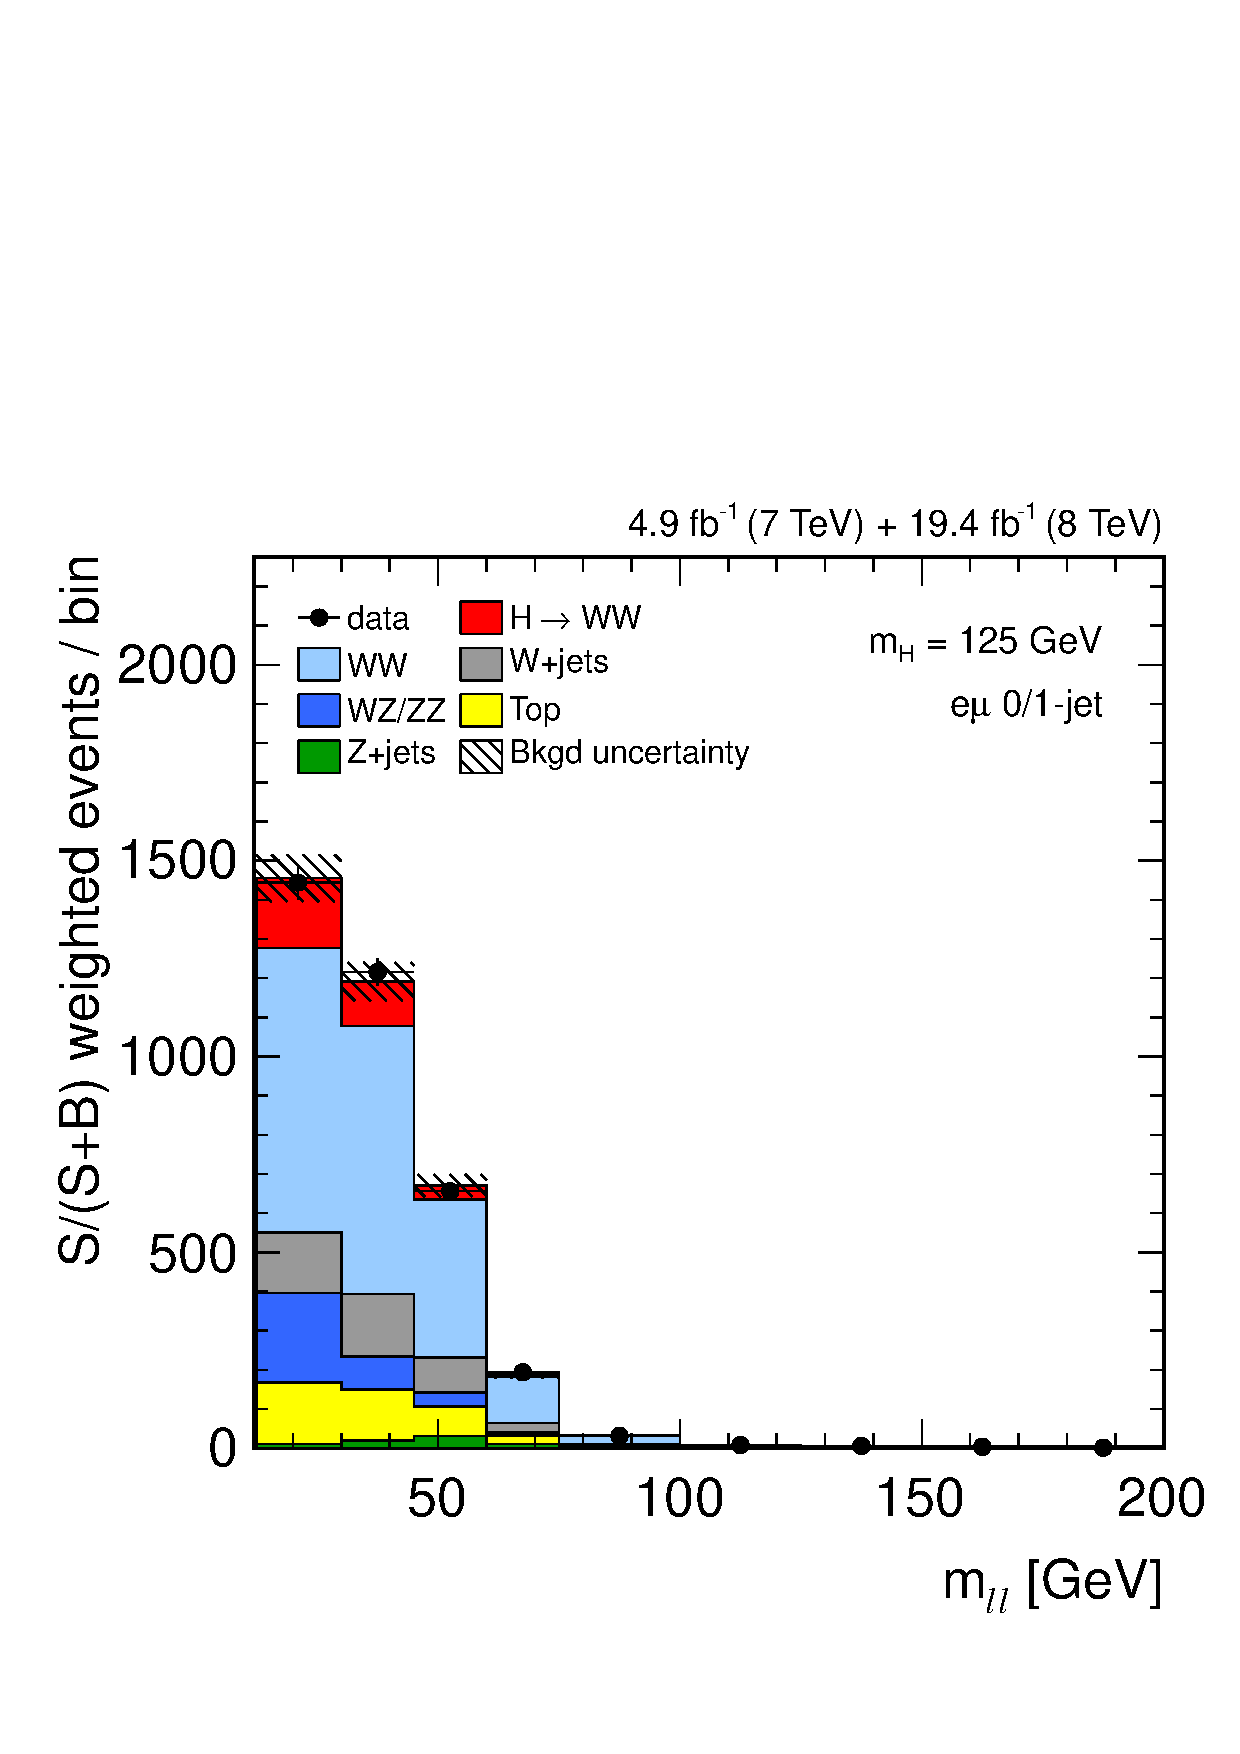
\includegraphics[width=0.49\textwidth]{figures/st_mll_2dweight.pdf}
%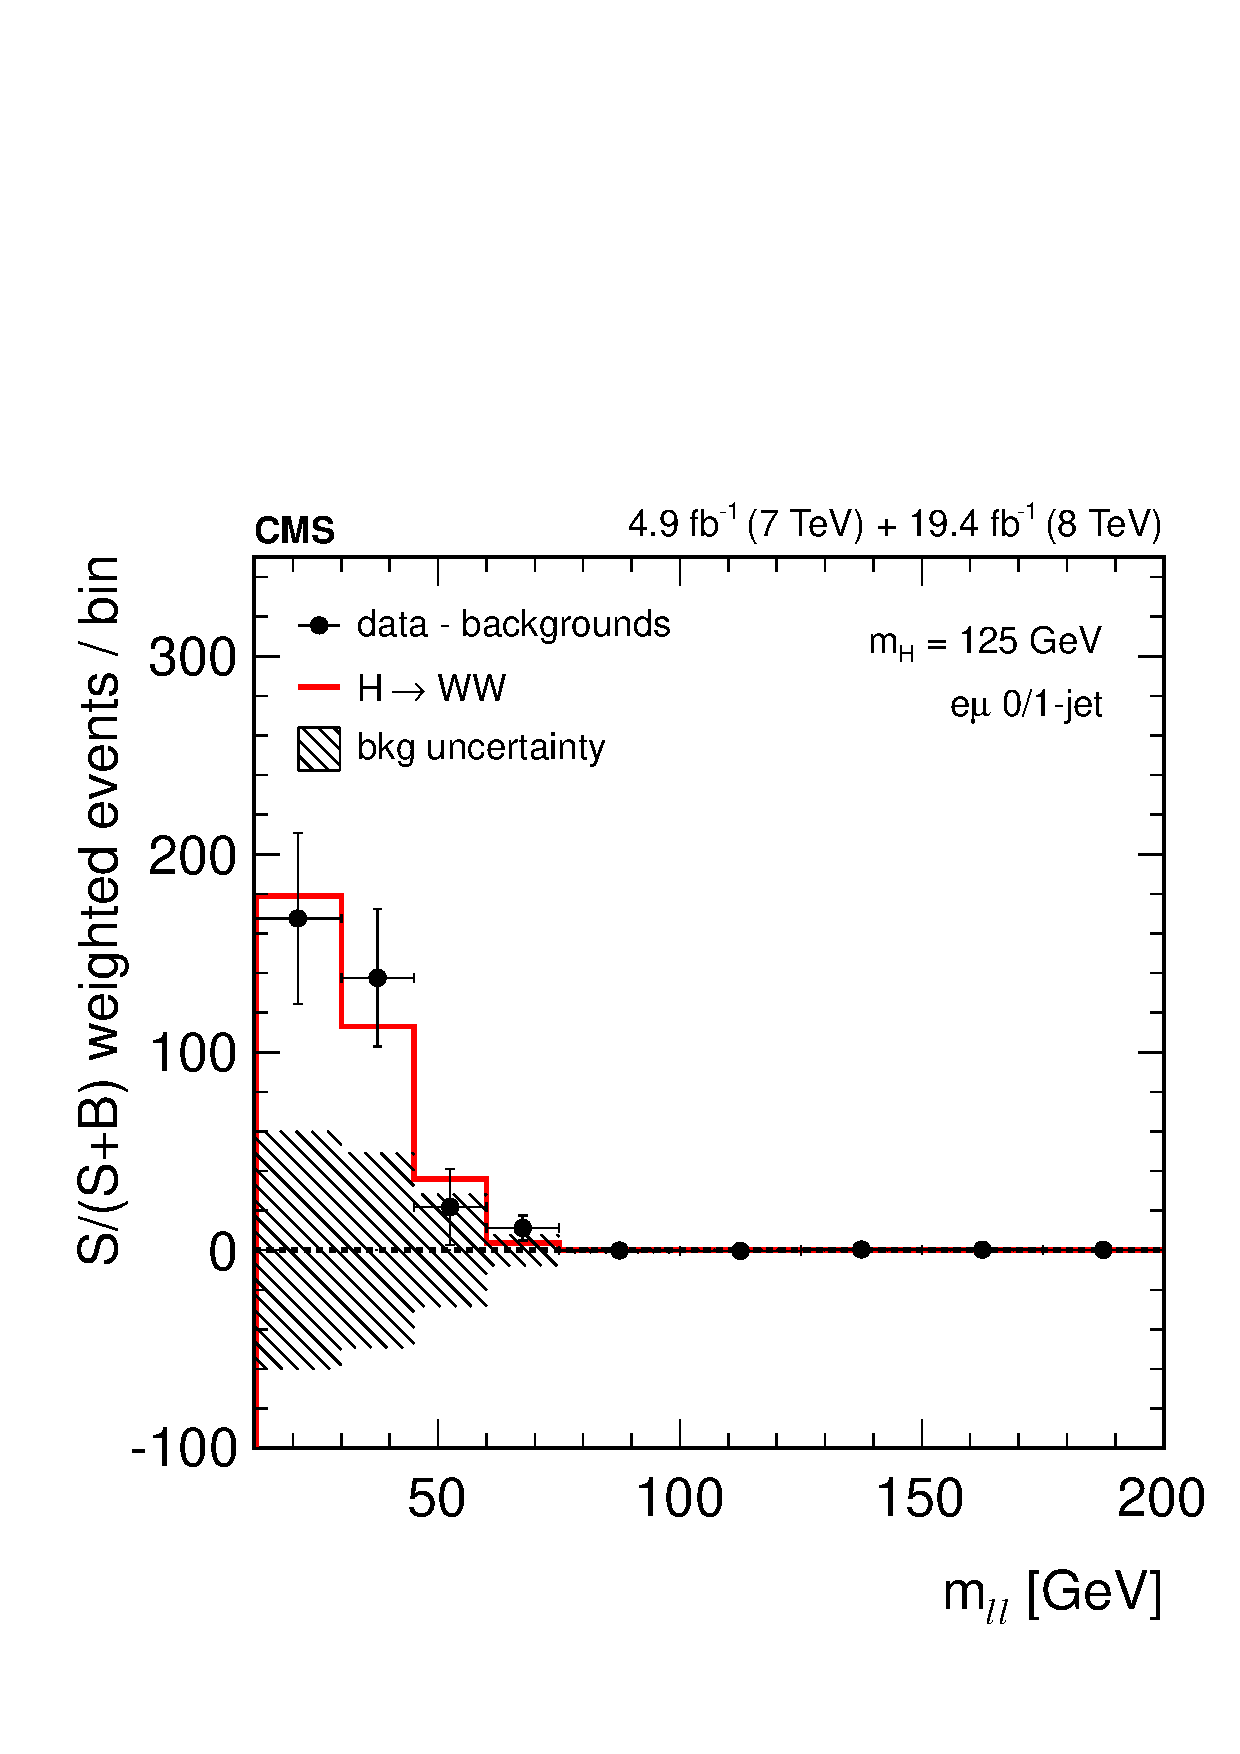
\includegraphics[width=0.49\textwidth]{figures/dataminusbkg_mll_2dweight.pdf} 
%\end{tabular} 
%\caption{\mT(top) and \mll(bottom) distributions using post-fit results 
%of shape-based analysis in \DF\ final states combining 7 and 8~\TeV.
%The signal and data subtracted by backgrounds are compared. 
%In order to give more weights to sensitivie category, each bin of 2D 
%template is weighted by S/(S+B) and the total yield is normalized using the signal yield. 
%Both normalization and shape of data show a very good agreement with SM Higgs at 125~\GeV. } 
%\label{fig:post1Dprojection_1dweight} 
%\end{figure} 

%%%%%%
\section{Exclusion limit of SM Higgs boson}  

Following the procedure described in section~\ref{sec:stat_exclusion}, 
we calculate the 95 \% \CLs\ limit on the signal strength, 
the ratio of observed signal yield to the expected signal yield 
at a given Higgs mass. The expected median limit and its $1\sigma$/$2\sigma$ uncertainty
bands are shown in yellow and green, respectively, along with the observed limit. 

Figure~\ref{fig:limit78} shows the exclusion limits of SM Higgs boson combining 
all categories in 7 and 8~\TeV. 
The top is the result using only cut-based results in all categories. 
The observed and expected exclusions of SM boson at \CLs = 95 \% are 
132 - 212 and 310 - 550~\GeV, and 120 - 480~\GeV, respectively. 
The bottom is the result of the cut-based method in the \SF\ category 
and the shape-based method in the \DF\ category.
The observed and expected exclusions of SM boson at \CLs = 95 \% are 
128-600~\GeV\ and 115-575~\GeV, respectively. 

Figure~\ref{fig:limit78_secondhiggs} shows the exclusion limit of 
the second SM-Higgs-like boson considering a SM Higgs at \mHi=125~\GeV\ as a backgound.
The cut-based result is used in \SF\ category 
and the shape-based result is used in \DF\ category.
The observed and expected exclusions of the second SM-Higgs-like boson at \CLs = 95 \% 
are 118-600~\GeV\ and 115-600~\GeV, respectively. 

\begin{figure}[htp] 
\centering 
\begin{tabular}{c} 
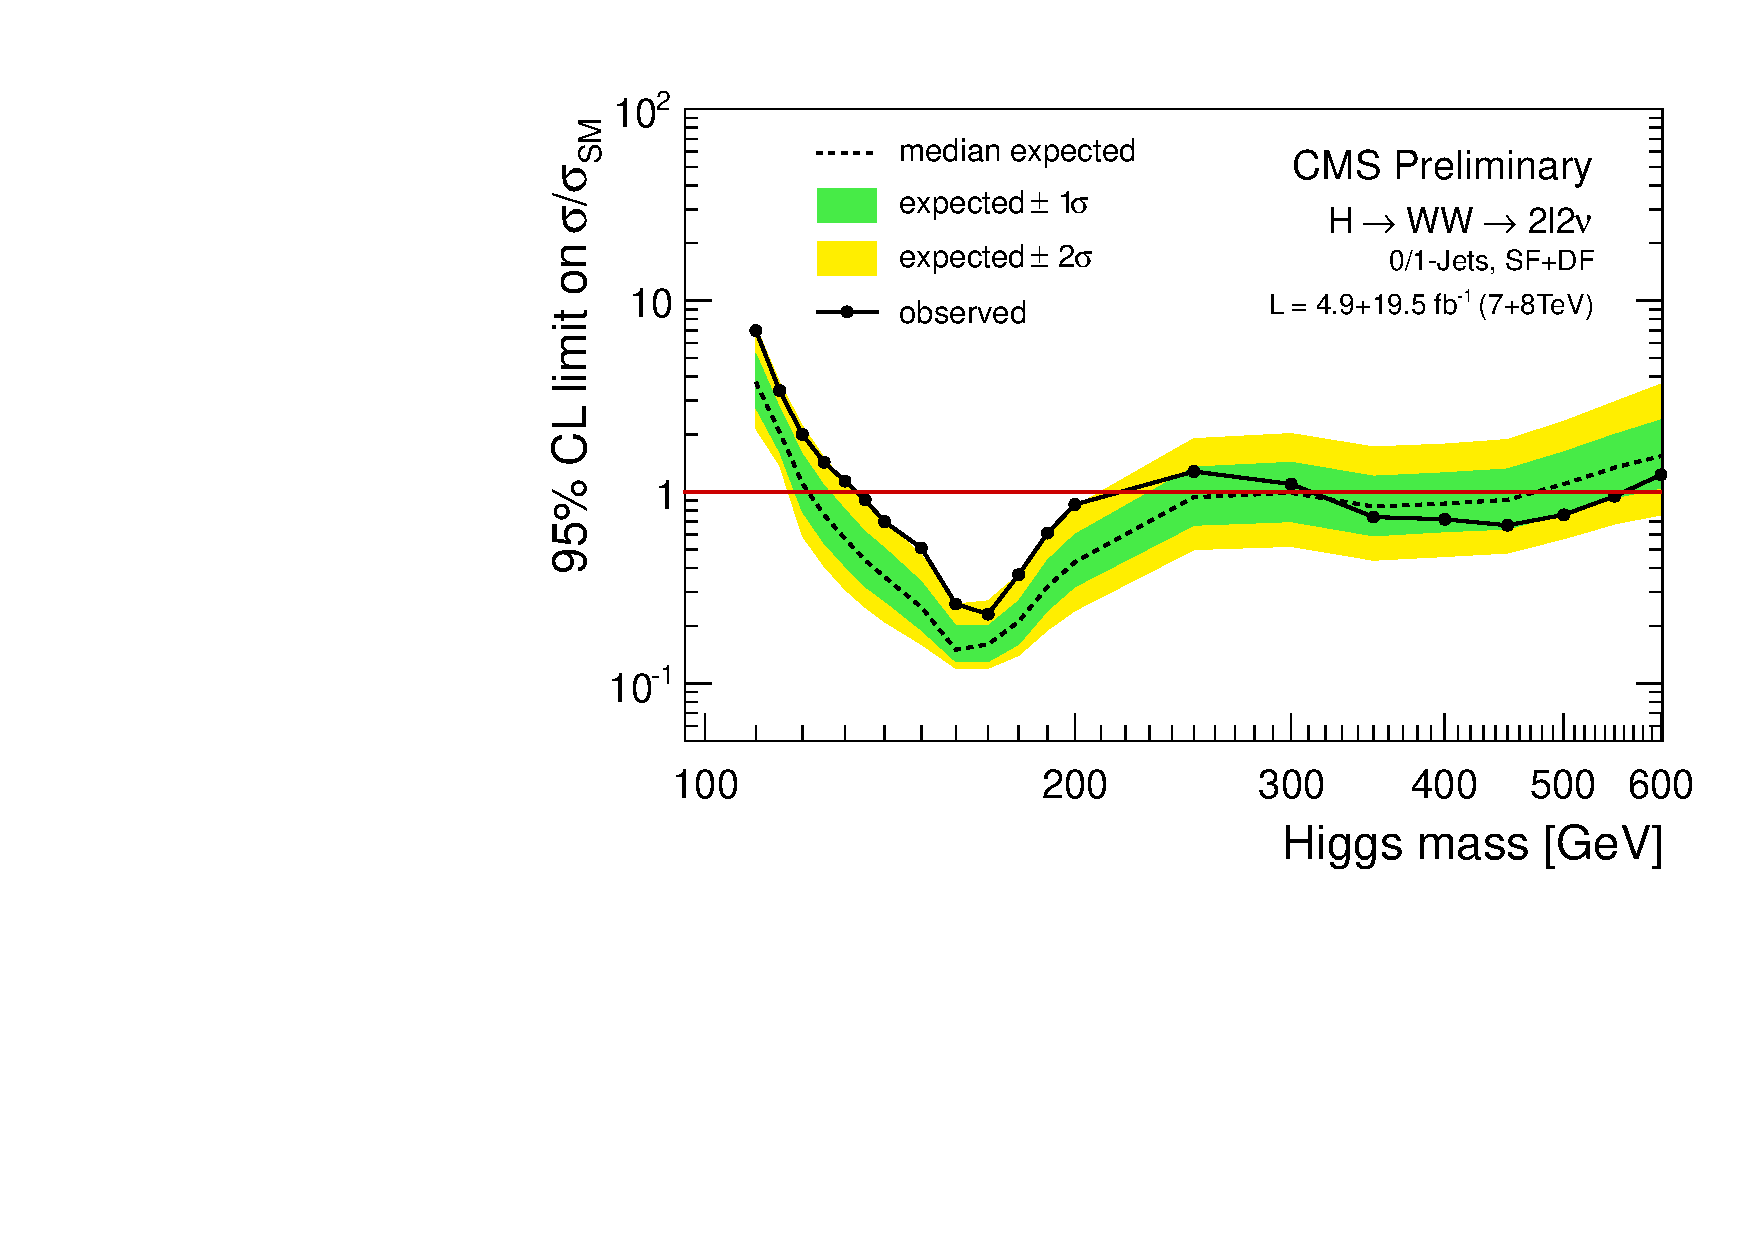
\includegraphics[width=0.9\textwidth]{figures/table_limits_nj_cut_78TeV_log.pdf} \\
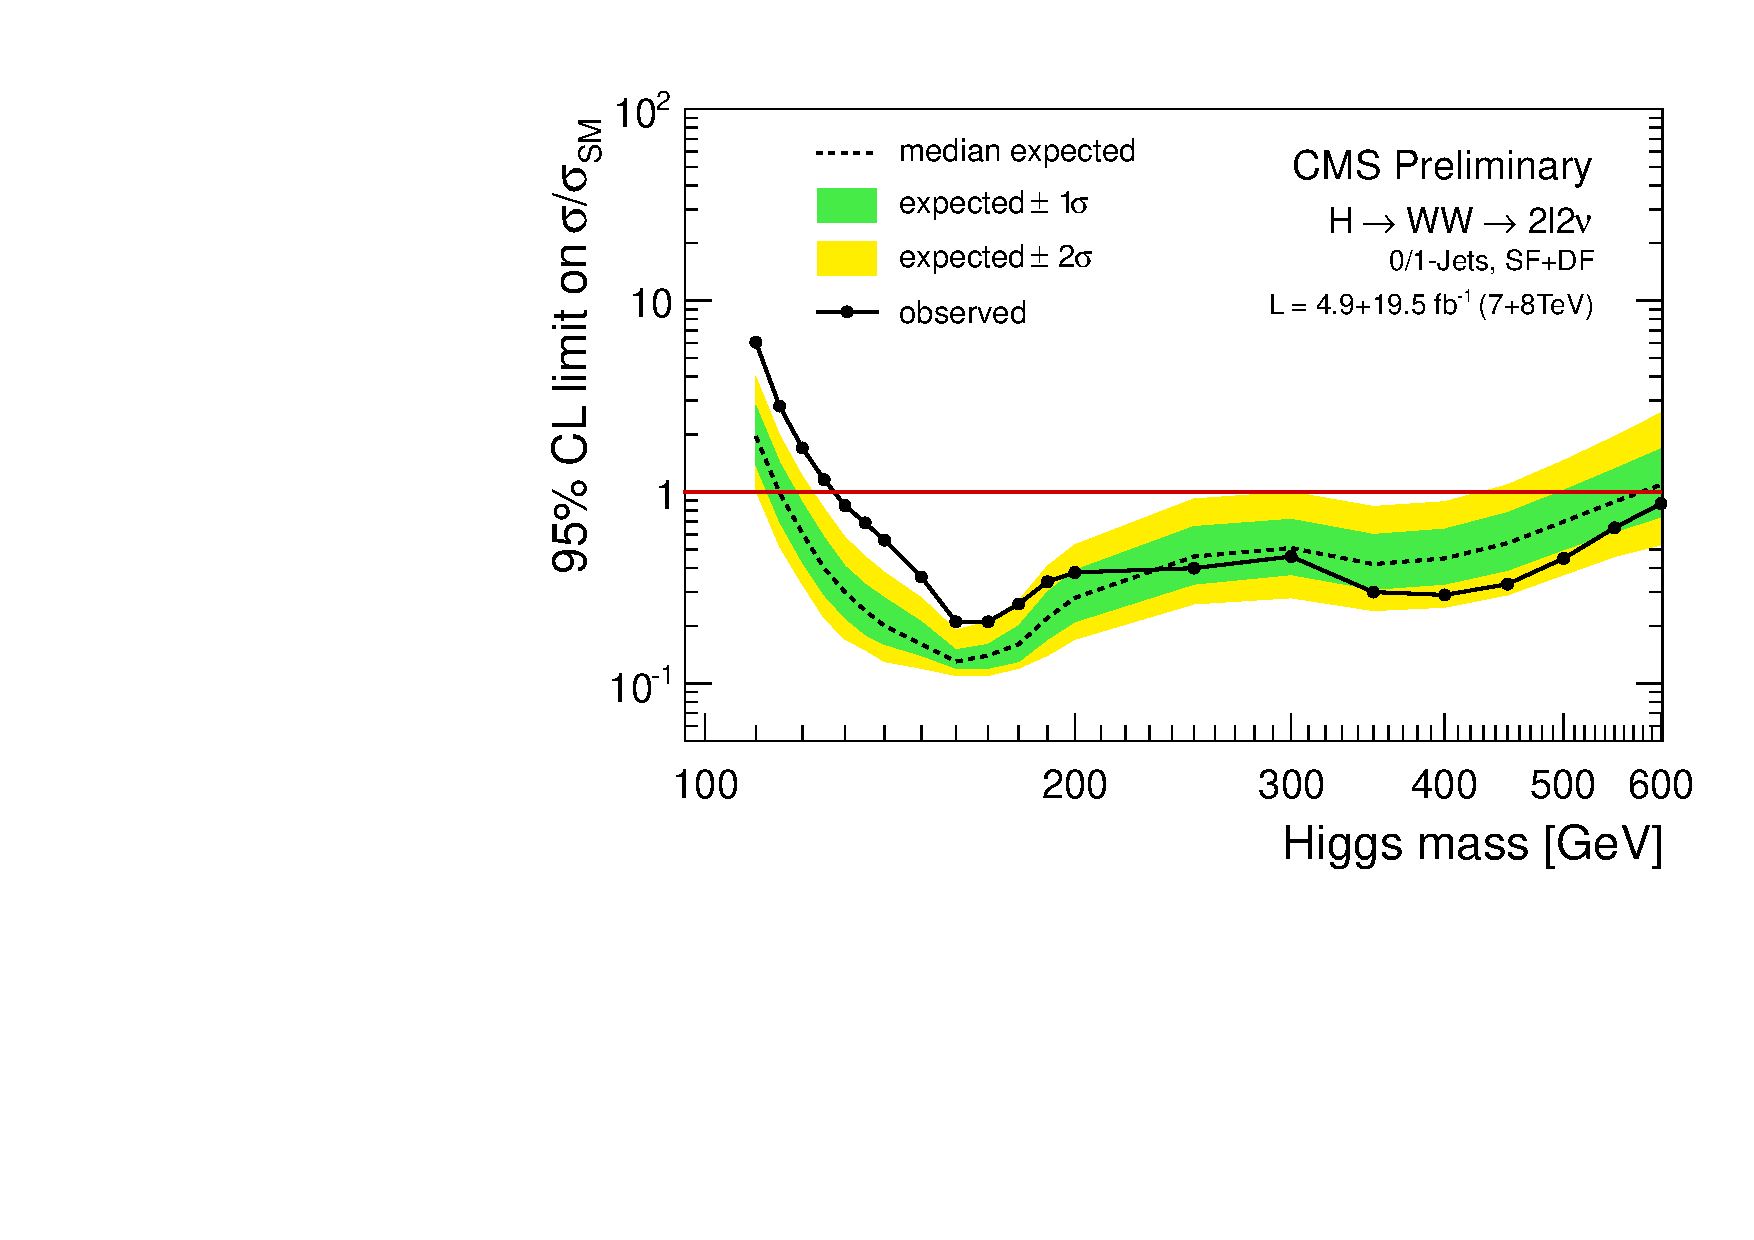
\includegraphics[width=0.9\textwidth]{figures/table_limits_nj_78TeV_log.pdf} 
\end{tabular} 
\caption{Exclusion limits of SM Higgs boson combining all categories in 7 and 8~\TeV. 
The top is the result of the cut-based method in all categories.
The observed and expected exclusions of SM boson at \CLs = 95 \% are 
132-212~\GeV\ and 120-480~\GeV, respectively. 
The bottom is the result of the cut-based method in \SF\ category 
and the shape-based method in \DF\ category.
The observed and expected exclusions of SM boson at \CLs = 95 \% are 
128-600~\GeV\ and 115-575~\GeV, respectively.} 
\label{fig:limit78} 
\end{figure} 

\begin{figure}[htp] 
\centering 
\begin{tabular}{c} 
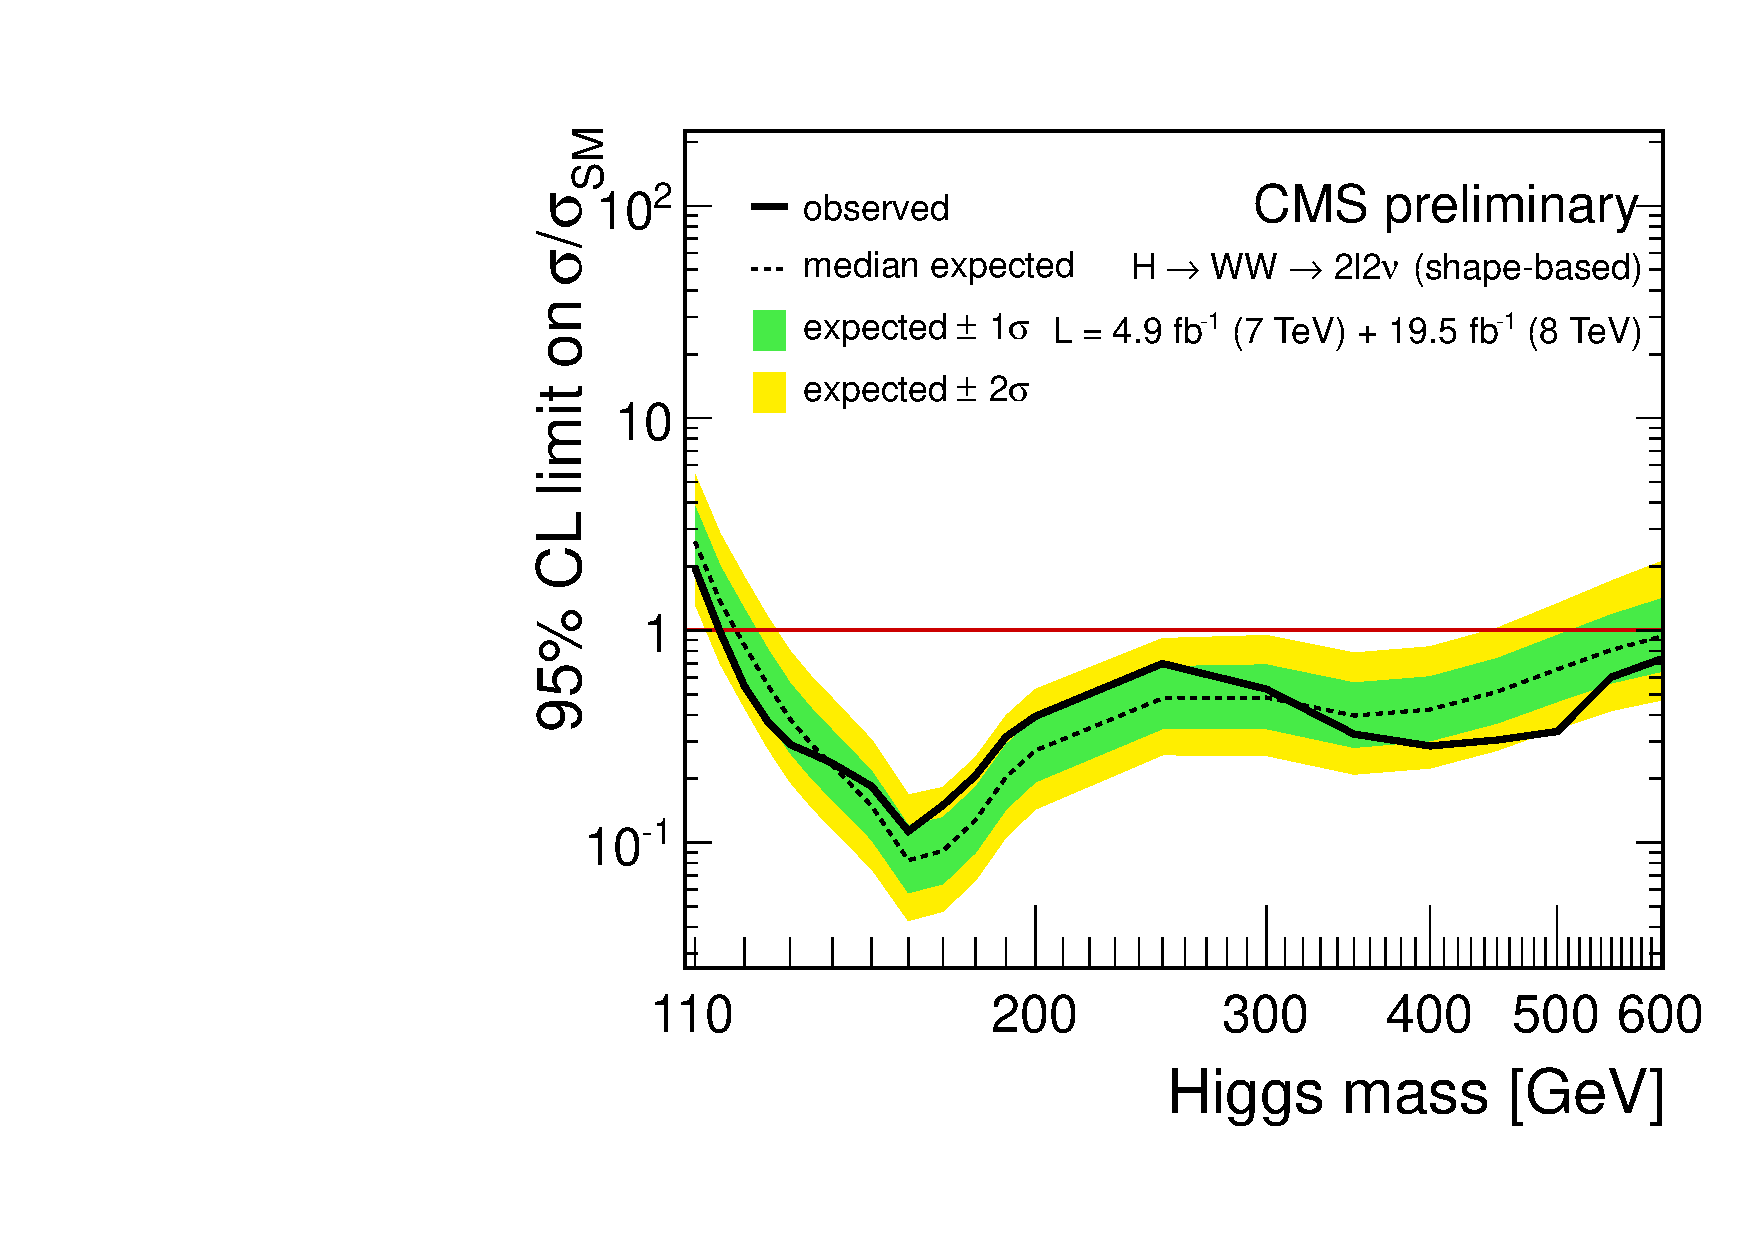
\includegraphics[width=0.9\textwidth]{figures/ana_Moriond13_2D_SMH_7p8TeV_bdt_from110to600_logx1_logy1.pdf} 
\end{tabular} 
\caption{Exclusion limit of the second SM-Higgs-like boson considering the 
SM Higgs at \mHi=125~\GeV\ as a backgound.
The cut-based method is used in \SF\ category and the shape-based method 
is used in \DF\ category.
The observed and expected exclusions of the second SM-Higgs-like boson at \CLs = 95 \% 
are 118-600~\GeV\ and 115-600~\GeV, respectively.} 
\label{fig:limit78_secondhiggs} 
\end{figure} 




\section{Discovery of a new boson}

Following the procedure described in section~\ref{sec:stat_significance}, 
we study the compatibility of data with the background-only hypothesis. 
The measure is expressed as significance. A Large deviation indicates 
that there is additional contribution on top of backgrounds. 
In this section, the expected and observed significances are shown
for selective mass points, $\mHi = 125, 160, 200, 400 \textrm{ and } 600~\GeV$.  

Tables~\ref{tab:significance_7tev} - \ref{tab:significance_78tev}  
show observed and expected significances at the selected \mHi, 
for 7~\TeV, 8~\TeV and combination of 7 and 8~\TeV.
The cut-based method is used in \SF\ category 
and the shape-based method is used in \DF\ category.
At \mHi=125~\GeV, the observed and expected significances
are $4.0\sigma$ and $5.2\sigma$, respectively, 
when all categories are combined.

Figure~\ref{fig:significane_mH} shows the observed and expected 
significance for low Higgs mass hypotheses($\mHi\le200~\GeV$). 
The solid black line represents the expected significance assuming 
\mHi = 125~\GeV\ signal. 
The green and yellow bands respresent the $1\sigma$/$2\sigma$ uncertainty 
band of the expected significance sestimated by pseudo data. 
The dotted line represents the significance 
assuming existence of SM Higgs at the given mass. 
The blue line is the observed significance. 
The observed data is within $1\sigma$ of the expected significance 
assuming the existence of SM Higgs boson at \mHi = 125~\GeV.

Table~\ref{tab:sig_diffgenerator} shows the observed and expected significances 
using different generators for the \qqww\ process. Alternative generators, 
MC@NLO and Powheg, were used replacing the default generator, Madgraph.
The result shows that the significance is insensitive to the choice 
of the default generator, \textit{i.e.}, central shape of the \qqww\ background.  


%%%%%%%%
\begin{table}[!htbp]
\begin{center}
\begin{tabular}{c | c c | c c }
\hline \hline 
                 &  \multicolumn{2}{c|}{2D} & \multicolumn{2}{c}{Cut-based} \\
\hline
Higgs Mass(\GeV) & Observed & Expected & Observed & Expected  \\
\hline \hline
%110 & 2.6 & 0.6 & 0.5 & 0.4 \\
%115 & 2.4 & 1.1 & 0.3 & 0.8 \\
%120 & 2.3 & 1.7 & 0.4 & 1.2 \\
125 & 2.3 & 2.5 & 0.8 & 1.7 \\
%135 & 1.9 & 4.5 & 1.0 & 3.1 \\
%140 & 1.5 & 5.5 & 0.5 & 3.8 \\
%150 & 1.2 & 7.2 & 0.8 & 5.0 \\
160 & 0.9 & 10.4 & 0.0 & 8.2 \\
%170 & 0.0 & 9.8 & 0.0 & 7.9 \\
%180 & 0.0 & 7.2 & 0.0 & 5.9 \\
%190 & 0.0 & 5.3 & 0.0 & 4.0 \\
200 & 0.0 & 3.7 & 0.0 & 2.9 \\
%250 & 0.0 & 2.0 & 0.0 & 1.5 \\
%300 & 1.2 & 1.7 & 0.0 & 1.4 \\
%350 & 0.3 & 2.1 & 0.0 & 1.6 \\
400 & 0.2 & 1.9 & 0.0 & 1.5 \\
%450 & 0.0 & 1.6 & 0.0 & 1.4 \\
%500 & 0.2 & 1.3 & 0.0 & 1.1 \\
%550 & 0.9 & 1.1 & 0.0 & 0.9 \\
600 & 0.0 & 0.9 & 0.0 & 0.8 \\
\hline \hline
\end{tabular}
\caption{Observed and expected significances in 7~\TeV.   
Cut-based analysis is used in \SF\ final states 
and shape-based analysis is used in \DF\ finale states} 
\label{tab:significance_7tev}
\end{center}
\end{table} 

%%%%%%%%
\begin{table}[!htbp]
\begin{center}
\begin{tabular}{c | c c | c c }
\hline \hline 
                 &  \multicolumn{2}{c|}{2D} & \multicolumn{2}{c}{Cut-based} \\
\hline
Higgs Mass(\GeV) & Observed & Expected & Observed & Expected  \\
\hline \hline
%110 & 2.9 & 0.9 & 2.3 & 0.6 \\
%115 & 3.2 & 1.8 & 2.3 & 1.2 \\
%120 & 3.2 & 3.0 & 1.0 & 1.8 \\
125 & 3.5 & 4.7 & 2.1 & 2.6 \\
%130 & 3.8 & 6.5 & 2.5 & 3.4 \\
%135 & 4.2 & 8.3 & 2.6 & 4.4 \\
%140 & 4.5 & 10.1 & 2.5 & 5.2 \\
%150 & 4.3 & 14.1 & 2.8 & 7.4 \\
160 & 4.1 & 20.5 & 0.0 & 11.5 \\
%170 & 3.5 & 17.5 & 0.0 & 10.7 \\
%180 & 3.1 & 12.4 & 2.5 & 8.4 \\
%190 & 2.5 & 8.6 & 2.6 & 5.6 \\
200 & 1.4 & 6.9 & 2.5 & 4.3 \\
%250 & 0.0 & 3.8 & 1.2 & 2.0 \\
%300 & 0.0 & 3.5 & 0.2 & 1.9 \\
%350 & 0.0 & 4.0 & 0.0 & 2.2 \\
400 & 0.0 & 3.8 & 0.0 & 2.1 \\
%450 & 0.0 & 3.1 & 0.0 & 2.0 \\
%500 & 0.0 & 2.4 & 0.0 & 1.7 \\
%550 & 0.0 & 2.0 & 0.0 & 1.4 \\
600 & 0.0 & 1.8 & 0.0 & 1.3 \\
\hline \hline
\end{tabular}
\caption{Observed and expected significances in 8~\TeV.   
Cut-based analysis is used in \SF\ final states 
and shape-based analysis is used in \DF\ finale states} 
\label{tab:significance_8tev}
\end{center}
\end{table} 


%%%%%%%%
\begin{table}[!htbp]
\begin{center}
\begin{tabular}{c | c c | c c }
\hline \hline 
                 &  \multicolumn{2}{c|}{2D} & \multicolumn{2}{c}{Cut-based} \\
\hline
Higgs Mass(\GeV) & Observed & Expected & Observed & Expected  \\
\hline \hline
%110 & 3.7 & 1.1 & 2.1 & 0.6 \\
%115 & 3.8 & 2.0 & 2.1 & 1.2 \\
%120 & 3.8 & 3.3 & 1.9 & 1.8 \\
125 & 4.0 & 5.2 & 2.1 & 2.7 \\
%130 & 4.3 & 7.2 & 2.3 & 3.5 \\
%135 & 4.5 & 9.2 & 2.5 & 4.4 \\
%140 & 4.6 & 11.2 & 2.4 & 5.2 \\
%150 & 4.2 & 15.2 & 2.8 & 7.5 \\
160 & 4.0 & 22.0 & 2.8 & 11.6 \\
%170 & 3.2 & 18.9 & 2.1 & 10.7 \\
%180 & 2.7 & 13.1 & 2.4 & 8.4 \\
%190 & 2.0 & 9.1 & 2.4 & 5.6 \\
200 & 1.3 & 7.2 & 2.5 & 4.3 \\
%250 & 0.0 & 4.2 & 0.9 & 2.1 \\
%300 & 0.0 & 3.8 & 0.2 & 2.0 \\
%350 & 0.0 & 4.4 & 0.0 & 2.3 \\
400 & 0.0 & 4.1 & 0.0 & 2.2 \\
%450 & 0.0 & 3.4 & 0.0 & 2.1 \\
%500 & 0.0 & 2.7 & 0.0 & 1.8 \\
%550 & 0.0 & 2.2 & 0.0 & 1.5 \\
600 & 0.0 & 2.0 & 0.0 & 1.4 \\
\hline \hline
\end{tabular}
\caption{Observed and expected significances combining 7~\TeV\ and 8~\TeV\ results.  
Cut-based analysis is used in \SF\ final states 
and shape-based analysis is used in \DF\ finale states} 
\label{tab:significance_78tev}
\end{center}
\end{table} 

%
\begin{figure}[htp] 
\centering 
\begin{tabular}{c} 
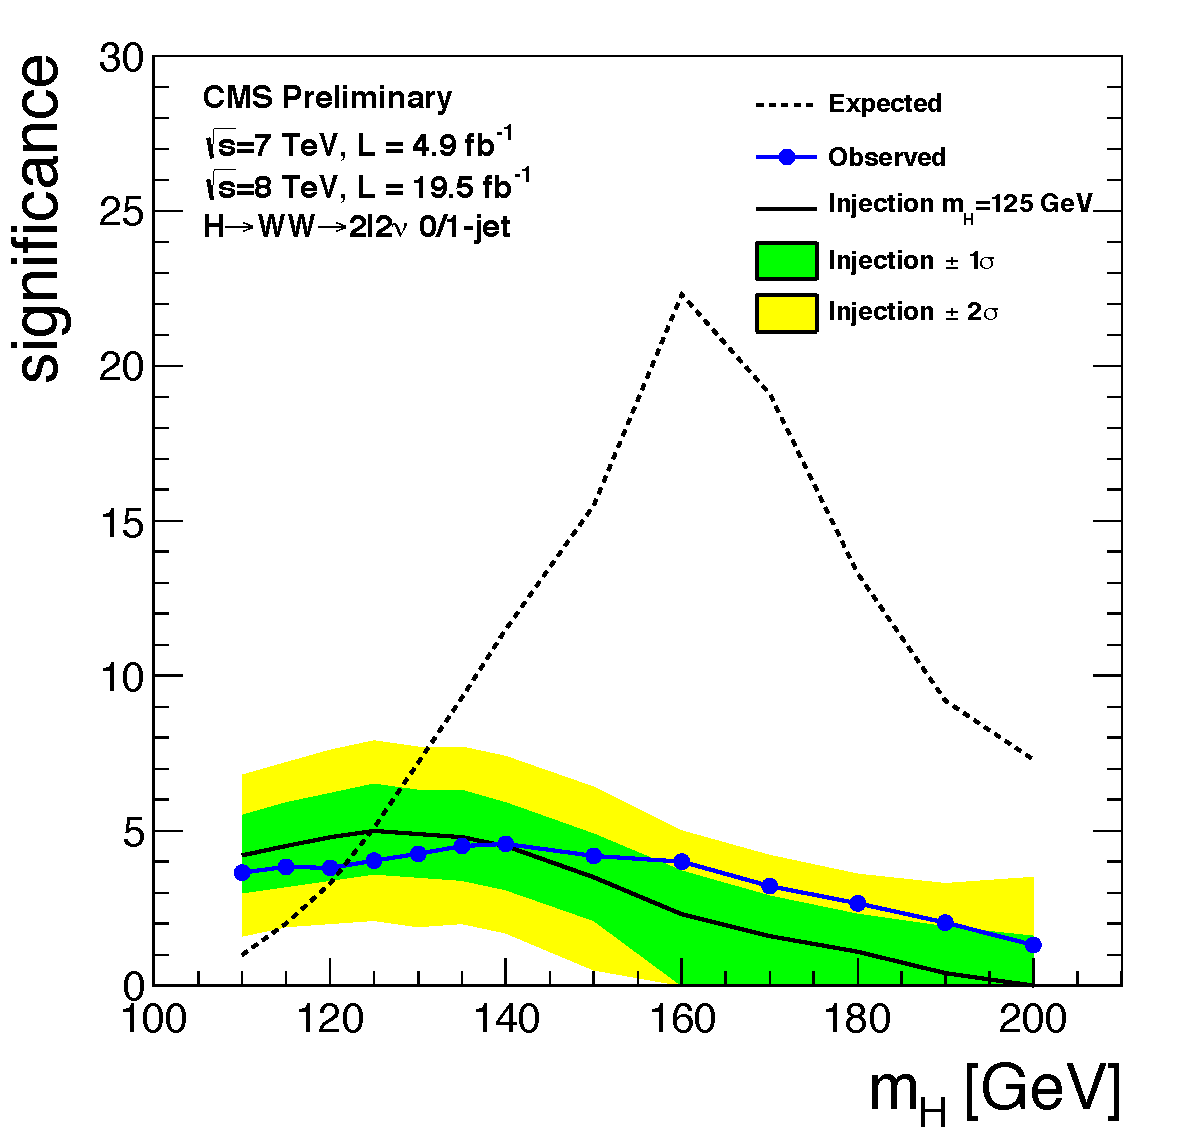
\includegraphics[width=0.8\textwidth]{figures/signif_allcomb_inj125_data_zoom.pdf} 
\end{tabular} 
\caption{Observed and expected significance as a function of \mHi\ for 
the low Higgs mass hypotheses($\mHi\le200~\GeV$). 
The solid black line represents the significance assuming \mHi = 125~\GeV\ signal. 
The green and yellow bands respresent $1\sigma$/$2\sigma$ uncertainty 
estimated by pseudo data. The dotted line represents the significance 
assuming existence of SM Higgs at the given mass. 
The blue line is the observed significance. 
} 
\label{fig:significane_mH} 
\end{figure} 

%
\begin{table}[htp] 
\begin{center} 
\begin{tabular}{cc|cc|cc} 
\hline 
\multicolumn{2}{c|}{MC@NLO}   &  \multicolumn{2}{c|}{Powheg} & \multicolumn{2}{c}{Madgraph} \\
\hline \hline 
Observed & Expected & Observed & Expected &  Observed & Expected \\ 
\hline 
4.2 & 5.3 & 3.9 & 5.1 & 4.0 & 5.2 \\
\hline 
\end{tabular} 
\caption{The observed and expected significances
using different generators for the \qqww\ process. Alternative generators,
MC@NLO and Powheg, were used replacing the default generator, Madgraph.
The result shows that the significance is insensitive to the choice
of default generator.} 
\label{tab:sig_diffgenerator} 
\end{center} 
\end{table} 


\section{Meausrement of Production rate($\sigma \times BR$)}

As mentioned before, we measure the signal strength at the 
measured Higgs mass. The mass measurement comes from 
$H\rightarrow ZZ\rightarrow4l$ and $H\rightarrow \gamma\gamma$, 
and it turned out to be around 125~\GeV~\cite{Chatrchyan:1637951, CMS-PAS-HIG-13-001}. 
For the results shown in this section,   
the cut-based analysis is used in \SF\ final states 
and shape-based analysis is used in \DF\ finale states. 

%fixme 
Figure~\ref{fig:mu_mH} shows the best fit signal strength 
as a function of \mHi\ for the low Higgs mass hypotheses($\mHi\le200~\GeV$)
using all categories in 7~\TeV\ and 8~\TeV. 
The green band shows $1\sigma$ error of the global fit. 
The signal strength is within $1\sigma$ of SM Higgs production rate 
in the range \mHi = 118 - 125~\GeV. 
Since the exact measured \mHi\ is $125.6~\GeV$~\cite{Chatrchyan:1637951}, 
we need to know how the signal strength is sensitive to the 
variation of \mHi\ around 125~\GeV. 
The signal strength at \mHi=126~\GeV\ and \mHi=124~\GeV\ are 0.82 and 0.72, respectively.

Figure~\ref{fig:mu_scan} shows the  $- 2\Delta\ln \mathcal{L}$ scan of $\mu$. 
The black curve represents the case where both systematic and statistical 
uncertainties are taken into account, while the blue curve represents the case 
where only statistical uncertainty is considered. To obtain the latter,  
all nuisances are fixed to the post-fit values, and fitted again.  
The uncertainty for the blue curve comes solely from statistics of data. 
The red lines represent the $1\sigma$ unceratinty band for each curve. 
The measured signal strength is $0.76 \pm 0.21$.  
One can extract the contribution of systematic uncertainties to the signal strength
by subtracting uncertainty in blue from the uncertainty in black.
Separating the systematic and statistical uncertainties, 
the measured signal strength is $0.76 \pm 0.16(syst.) \pm 0.13(stat.)$.  

Figure~\ref{fig:mu_allchannels} shows the fitted signal strength($\mu$) 
for \mHi=125~\GeV in the individual category. 
The dotted vertical line and the green band are 
the central value and the uncertainty band of the signal strength, respectively, 
obtained from the combination of all categories. 
The figure shows that all categories are consistent with each other
within the uncertainties.

Table~\ref{tab:mu_diffgenerator} shows the signal strengths 
using different generators for the \qqww\ process. Alternative generators,
MC@NLO and Powheg, are used replacing the default generator, Madgraph.
The result shows that the signal strength is insensitive to the choice
of default generator. 


%
\begin{figure}[htp] 
\centering 
\begin{tabular}{c} 
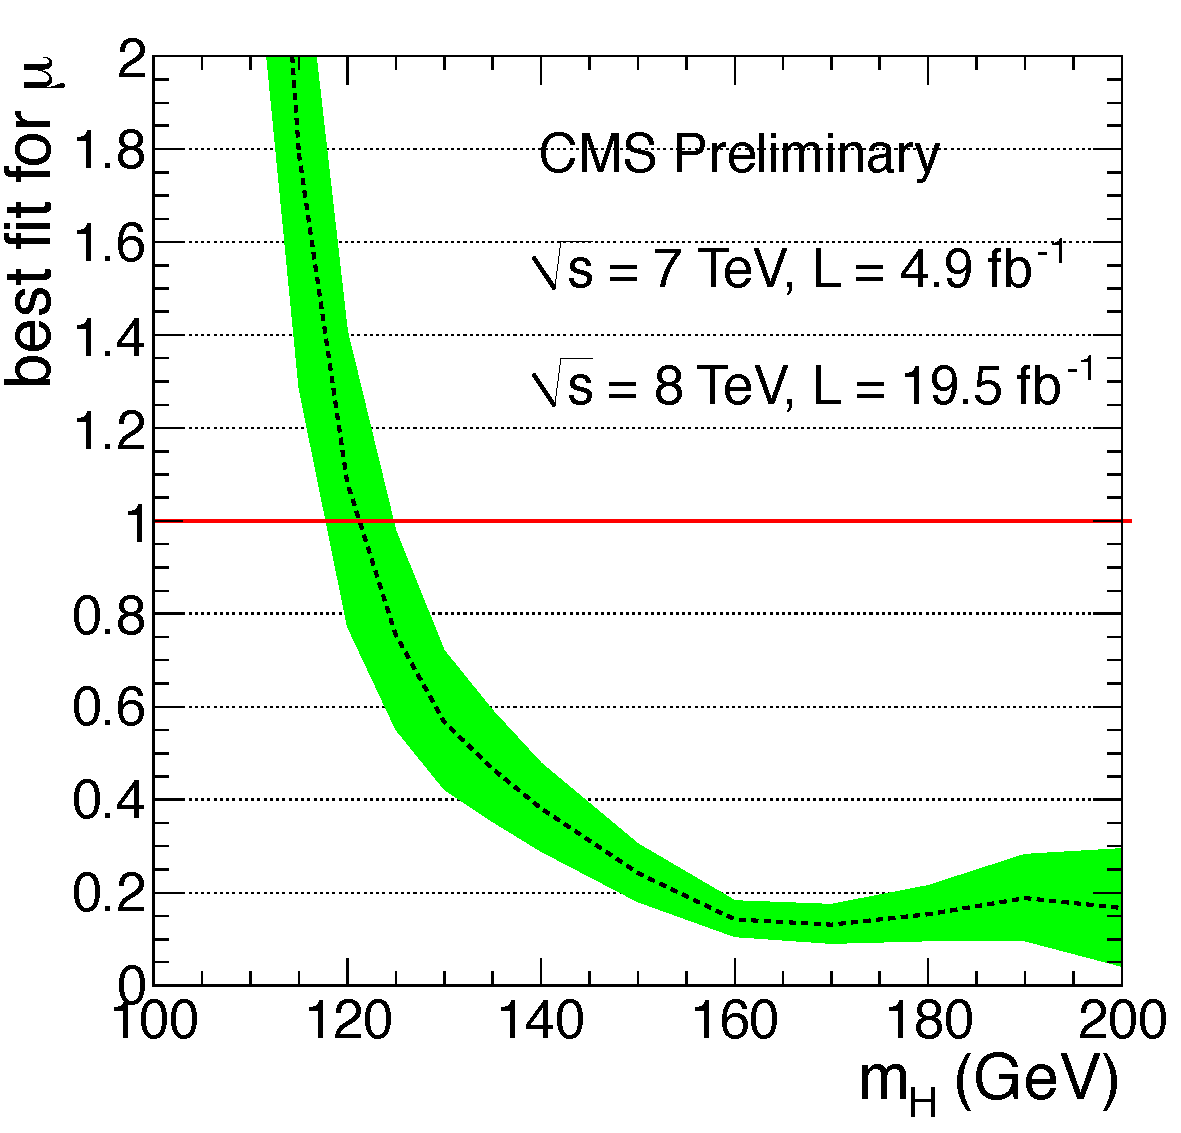
\includegraphics[width=0.8\textwidth]{figures/mlf7p8TeV_zoomed.pdf}
\end{tabular} 
\caption{The best fit signal strength($\mu$) as a function of \mHi\ for low Higgs 
mass hypotheses($\mHi\le200~\GeV$).
all categories are combined. 
Cut-based analysis is used in \SF\ final states 
and shape-based analysis is used in \DF\ finale states} 
\label{fig:mu_mH} 
\end{figure} 

%
\begin{figure}[htp] 
\centering 
\begin{tabular}{c} 
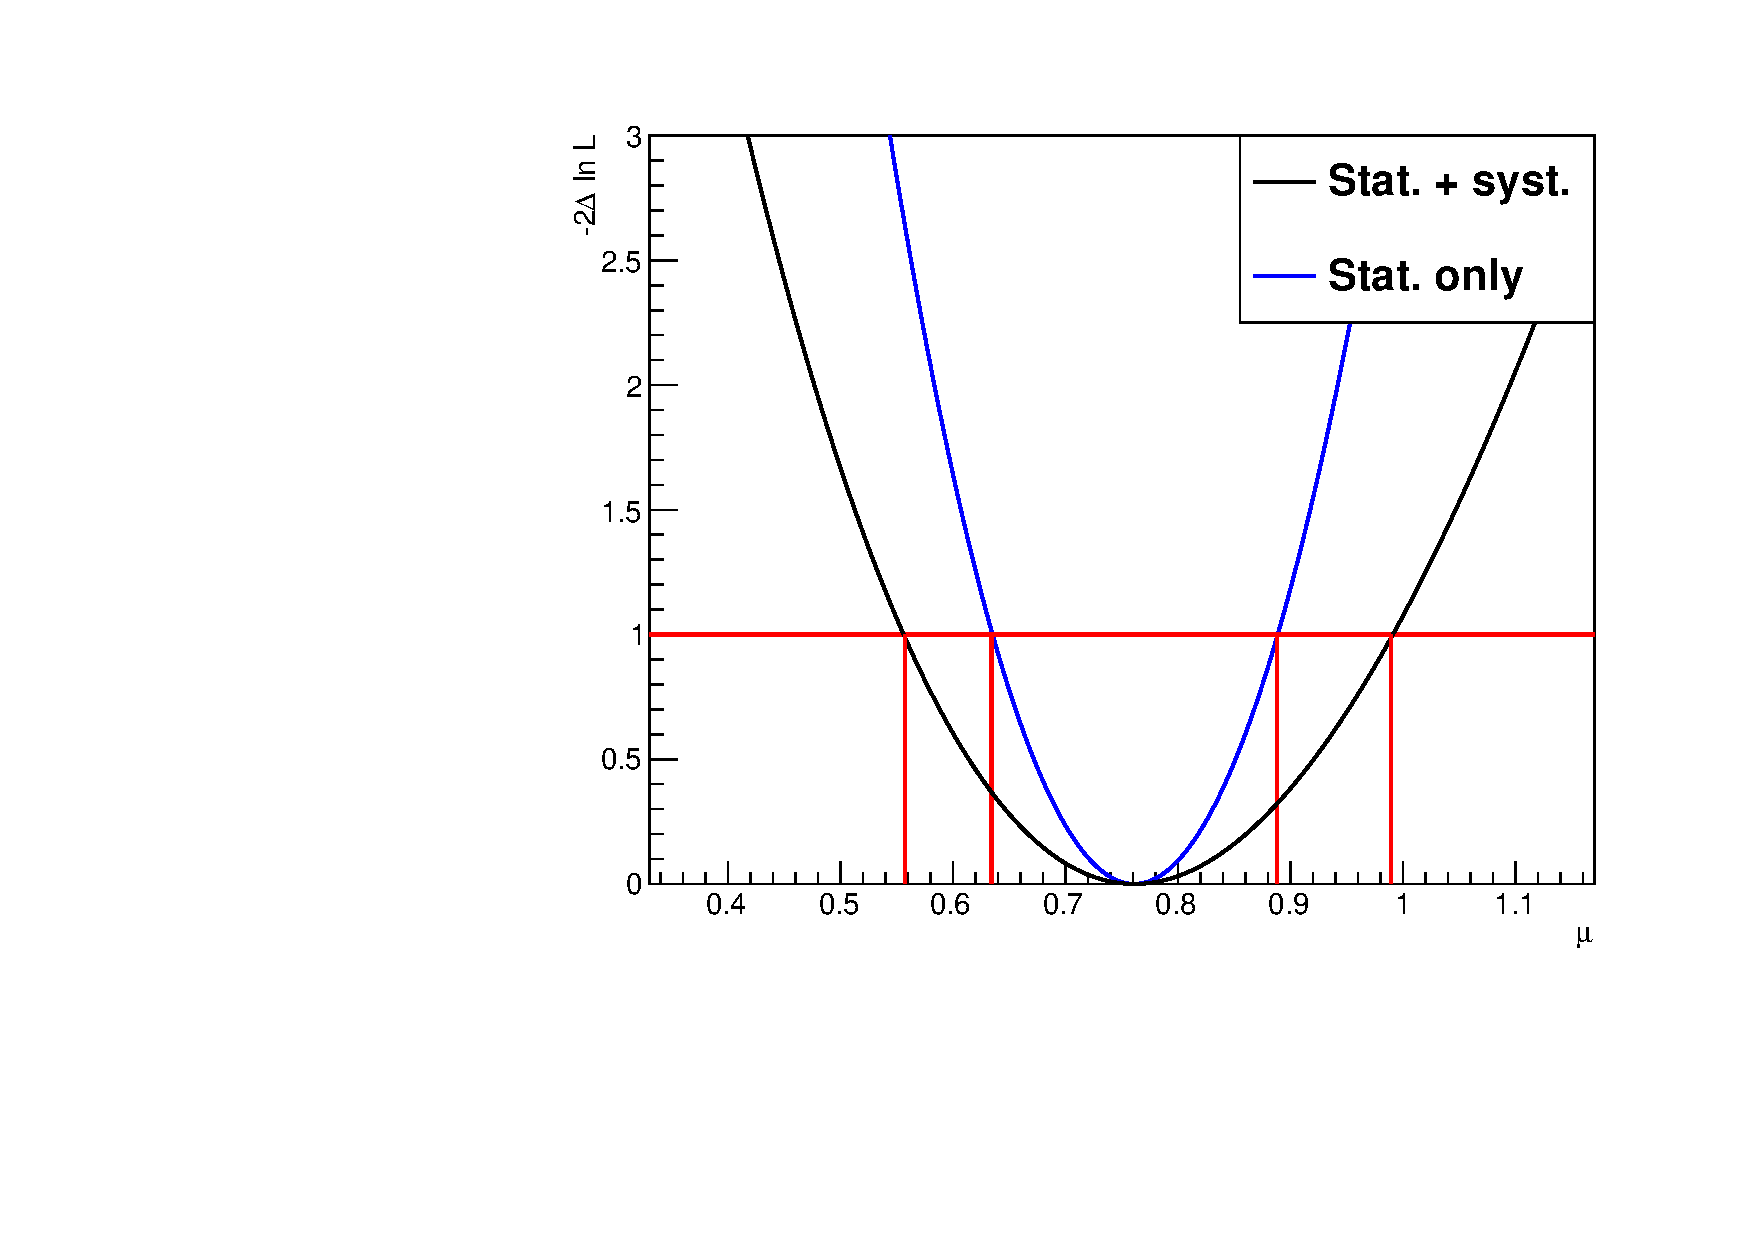
\includegraphics[width=0.8\textwidth]{figures/MuDeltaNLL.pdf}
\end{tabular} 
\caption{ $- 2\Delta\ln \textrm{L}$ scan of $\mu$ with(black) 
and without(blue) systematic uncertainty.
The uncertainty for the blue curve comes solely from statistics of data.
The red lines represent the $1\sigma$ unceratinty band for each curve. 
One can extract the contribution of systematic uncertainties to the signal strength
by subtracting uncertainty in blue from the uncertainty in black.} 
\label{fig:mu_scan} 
\end{figure} 

%
\begin{figure}[htp] 
\centering 
\begin{tabular}{c} 
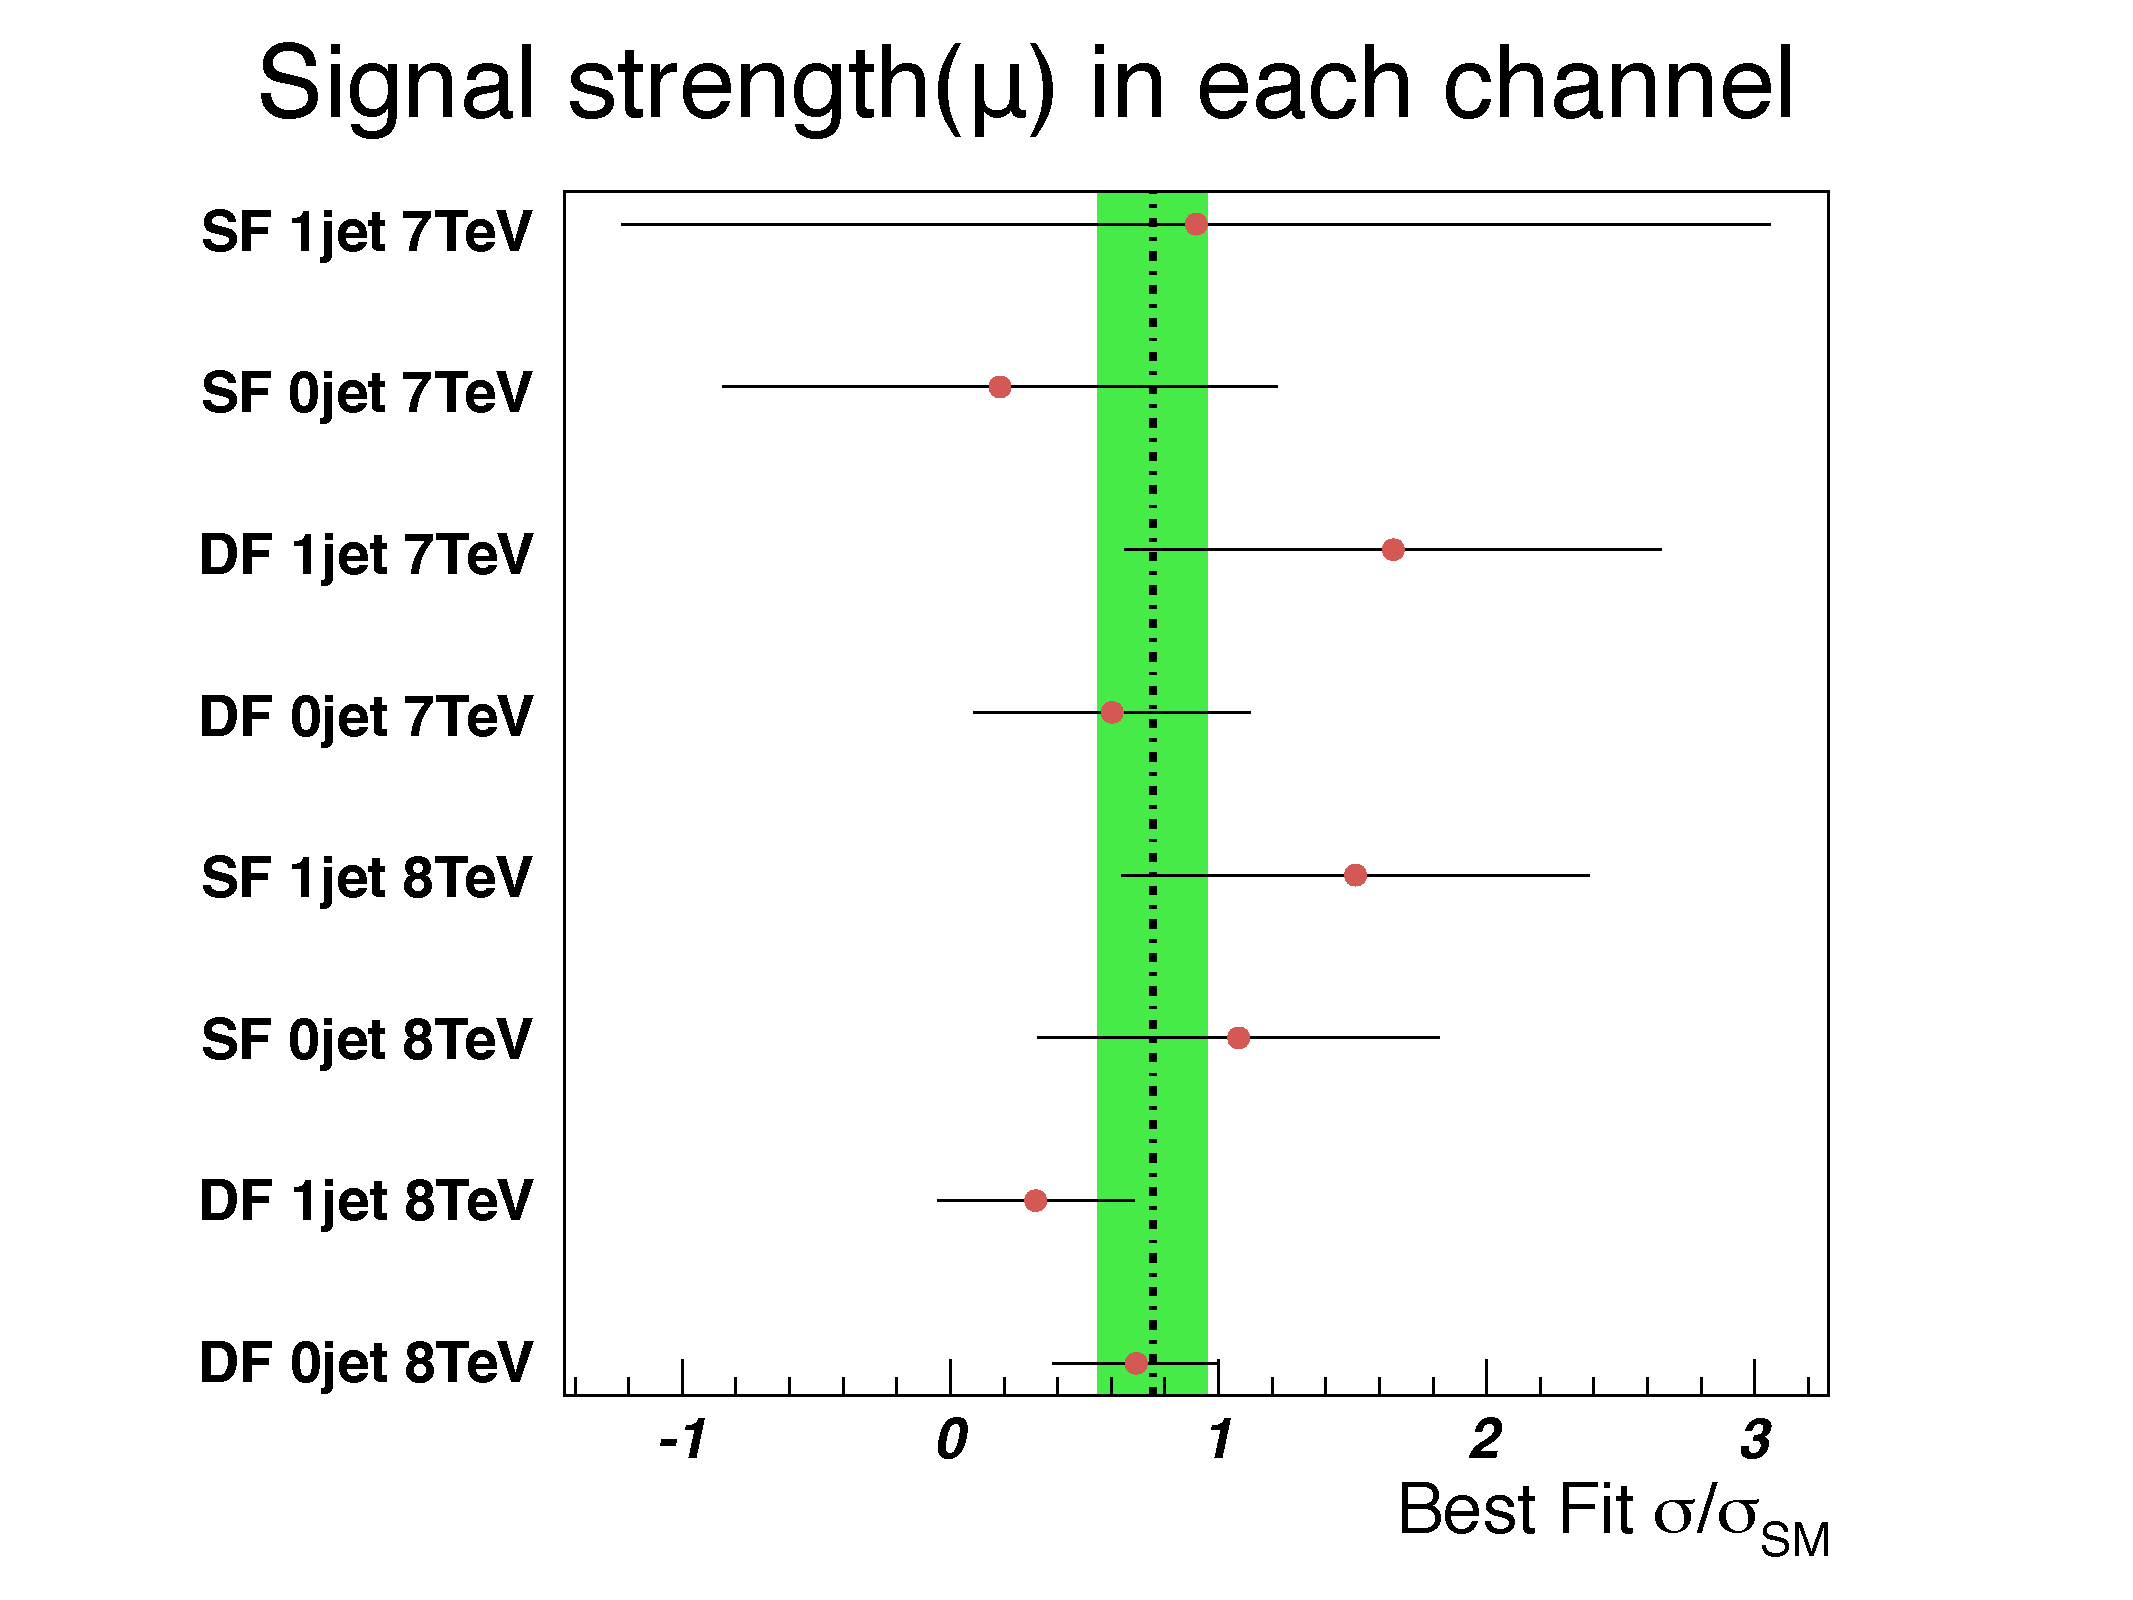
\includegraphics[width=0.99\textwidth]{figures/mu_allchannels.pdf}
\end{tabular} 
\caption{ Signal strength($\mu$) for individual category for \mHi=125~\GeV.
Cut-based analysis is used in \SF\ final states 
and shape-based analysis is used in \DF\ finale states. 
The dotted vertical line and the green band are 
the central value and uncertainty band of the signal strength 
obtained from combination of all categories. 
all categories are consistent to each other.
} 
\label{fig:mu_allchannels} 
\end{figure} 

%
\begin{table}[htp] 
\begin{center} 
\begin{tabular}{c|c|c} 
\hline 
MC@NLO   &  Powheg & Madgraph \\
\hline \hline 
$0.82 \pm 0.24$ & $0.74 \pm 0.21$ & $0.76 \pm 0.21$ \\
\hline 
\end{tabular} 
\caption{ Signal strengths 
using different generators for the \qqww\ process. Alternative generators,
MC@NLO and Powheg, were used replacing the default generator, Madgraph.
The result shows that the significance is insensitive to the choice
of default generator.} 
\label{tab:mu_diffgenerator} 
\end{center} 
\end{table} 



